%beamer 

%\PassOptionsToClass{handout}{beamer}

% \newboolean{handoutmode}
% \setboolean{handoutmode}{false}
%\newcommand{\handoutmode}{}

%% LaTeX-Beamer template for KIT design
%% by Erik Burger, Christian Hammer
%% title picture by Klaus Krogmann
%%
%% version 2.1
%%
%% mostly compatible to KIT corporate design v2.0
%% http://intranet.kit.edu/gestaltungsrichtlinien.php
%%
%% Problems, bugs and comments to
%% burger@kit.edu
\ifdefined \handoutmode
\documentclass[18pt, handout]{beamer}
\else
\documentclass[18pt]{beamer}
\fi

\usepackage[T1]{fontenc}
\usepackage[utf8]{inputenc}

\usepackage{../preamble/templates/beamerthemekit}

\usepackage[vlined]{algorithm2e}  %possible: noend, noline, ...
\usepackage{amssymb}
\usepackage{amsmath}
\usepackage{wasysym}
\usepackage{graphicx}
%\usepackage{hyperref}
\usepackage[export]{adjustbox}
\usepackage{wrapfig}
\usepackage{colortbl}
\usepackage{tikz}
\usetikzlibrary{matrix}
\usetikzlibrary{arrows.meta}
\usetikzlibrary{automata}
\usetikzlibrary{tikzmark}
\graphicspath{{images/}}
%\usepackage[colorlinks=true,urlcolor=blue,linkcolor=blue]{hyperref}
\usepackage[outline]{contour}
\usepackage{cancel}
\usepackage[warn]{textcomp}
\usepackage{multicol}
\usepackage{tabularx}
\usepackage{xcolor}
\usepackage{hhline}
\usepackage{environ}
\usepackage{calc}
\usepackage{bm}
\usepackage{xspace} % for \xspace command
\usepackage{varwidth}
\usepackage{csquotes}

\newcommand{\mycomment}[1]{}

%%%% CONFIG

\input{../preamble/config.tex}

%%%% CONFIG END

%\renewcommand{\SS}{\iffontchar\font"1E9E \symbol{"1E9E}\else SS\fi} % SHAME ON YOU, LATEX!
\newcommand{\TM}{\text{$\mbox{}^\text{\tiny TM}$}}
\newcommand{\pluseq}{\mathrel{+}=}
\newcommand{\pp}{\operatorname{++}} 
\newcommand{\mm}{\operatorname{--\mbox{\:}--}}
\newcommand{\minuseq}{\mathrel{-}=}
\newcommand{\asteq}{\mathrel{*}=}
\newcommand{\muleq}{\asteq}
\renewcommand{\mod}{\mathop{\textbf{mod}}} 
\renewcommand{\div}{\mathop{\textbf{div}}}
\newcommand{\N}{\mathbb{N}} 
\newcommand{\R}{\mathbb{R}}
\newcommand{\Z}{\mathbb{Z}}
\newcommand{\E}{\mathbb{E}}
\renewcommand{\P}{\mathbb{P}}
\newcommand{\BB}{\mathbb{B}} % \B already exists
\newcommand{\NP}{\ensuremath{\mathcal{N\hspace{-1.5pt}P}}}
\newcommand{\Oh}[1]{\mathcal{O}\!\left(#1\right)}
\renewcommand{\O}{\mathcal{O}}
\newcommand{\Om}[1]{\Omega\!\left(#1\right)}
\newcommand{\Th}[1]{\Theta\!\left(#1\right)}

\newcommand{\realTilde}{\textasciitilde\xspace}
\renewcommand{\qedsymbol}{\textcolor{black}{\openbox}}

\newcommand{\size}[1]{\ensuremath{\left\lvert #1 \right\rvert}}
\newcommand{\set}[1]{\left\{#1\right\}}
\newcommand{\tuple}[1]{\left(#1\right)}

\newcommand*{\from}{\colon}

\newcommand{\morescalingdelimiters}{   % for proper \left( \right) typography
	\delimitershortfall=0pt  % formerly: 0pt  
	\delimiterfactor=1
}
% todo later
%\delimitershortfall=0pt  % for proper \left( \right) typography
%\delimiterfactor=1

% --- \frameheight constant ---
\newlength\fullframeheight
\newlength\framewithtitleheight
\setlength\fullframeheight{.92\textheight}
\setlength\framewithtitleheight{.86\textheight}

\newlength\frameheight
\setlength\frameheight{\fullframeheight}

\let\frametitleentry\relax
\let\oldframetitle\frametitle
\def\frametitle#1{\global\def\frametitleentry{#1}\if\relax\frametitleentry\relax\else\setlength\frameheight{\framewithtitleheight}\fi\oldframetitle{#1}}

% --- \frameheight constant end ---

\def\·{\cdot}
\def\*{\cdot}
\def\<{\langle}
\def\>{\rangle}


\newcommand{\zB}{z.\,B.\@\xspace}
\newcommand{\ZB}{Z.\,B.\@\xspace}

\newcommand{\ceil}[1]{\left\lceil#1\right\rceil}
\newcommand{\floor}[1]{\left\lfloor#1\right\rfloor}
\newcommand{\abs}[1]{\left|#1\right|}
\newcommand{\Matrix}[1]{\begin{pmatrix} #1 \end{pmatrix}}
\newcommand{\braced}[1]{\left\lbrace #1 \right\rbrace}
\newcommand{\llist}[1]{\langle #1 \rangle}
\newcommand{\Mid}{\;\middle|\;}

\let\after\circ

\newcommand{\entspr}{\ensuremath{\mathrel{\hat{=}}}\xspace}

\def\~~>{\ensuremath{\rightsquigarrow}}  % FuCKING FINALLY! :D

% "something" placeholder. Useful for repairing spacing of operator sections, like `\sth = 42`.
\def\sth{\vphantom{.}}

\def\fract#1/#2 {\frac{#1}{#2}}  % ! TRAILING SPACE is CRUCIAL!
\def\dfract#1/#2 {\dfrac{#1}{#2}} % ! Trailing space is crucial!

\newcommand{\tight}[1]{{\renewcommand{\arraystretch}{0.76} #1}}
\newcommand{\stackedtight}[1]{{\renewcommand{\arraystretch}{0.76} \begin{matrix} #1 \end{matrix}} }
\newcommand{\stacked}[1]{\begin{matrix} #1 \end{matrix} }
\newcommand{\casesl}[1]{\delimitershortfall=0pt  \left\lbrace\hspace{-.3\baselineskip}\begin{array}{ll} #1 \end{array}\right.}
\newcommand{\casesr}[1]{\delimitershortfall=0pt  \left.\begin{array}{ll} #1 \end{array}\right\rbrace}
\newcommand{\caseslr}[1]{\delimitershortfall=0pt  \left\lbrace\begin{array}{ll} #1 \end{array}\hspace{-.3\baselineskip}\right\rbrace}

\def\q#1uad{\ifnum#1=0\relax\else\quad\q{\the\numexpr#1-1\relax}uad\fi}
% e.g. \q1uad = \quad, \q2uad = \qquad etc.

\newcommand{\qqquad}{\q3uad}


\def\indentstring{}
\def\§#1{\def\indentstring{#1}#1}
\def\.{{$\hphantom{\text{\indentstring}}$}}


\newcommand{\impl}{\ifmmode\ensuremath{\mskip\thinmuskip\Rightarrow\mskip\thinmuskip}\else$\Rightarrow$\xspace\fi}  
\newcommand{\Impl}{\ifmmode\implies\else$\Longrightarrow$\xspace\fi}

\newcommand{\gdw}{\ifmmode\mskip\thickmuskip\Leftrightarrow\mskip\thickmuskip\else$\Leftrightarrow$\xspace\fi}
\newcommand{\Gdw}{\ifmmode\iff\else$\Longleftrightarrow$\xspace\fi}

\newcommand{\symbitemnegoffset}{\hspace{-.33\baselineskip}}
\newcommand{\implitem}{\item[\impl\symbitemnegoffset]}
\newcommand{\Implitem}{\item[\Impl\symbitemnegoffset]}


\newcommand{\forcenewline}{\mbox{}\\}

\newcommand{\bfalert}[1]{\textbf{\alert{#1}}}
\let\elem\in   % I'm a Haskell freak. Don't judge me. :P


\newenvironment{threealign}{%
	\[
	\begin{array}{r@{\ }c@{\ }l}
}{%
	\end{array}	
	\]
}


\makeatletter
% Provides color if undefined.
\newcommand{\colorprovide}[2]{%
	\@ifundefinedcolor{#1}{\colorlet{#1}{#2}}{}}
\makeatother



%\pgfdeclarelayer{background}
%\pgfdeclarelayer{foreground}
%\pgfsetlayers{background,main,foreground}

\colorprovide{lightred}{red!30}
\colorprovide{lightgreen}{green!40}
\colorprovide{lightyellow}{yellow!50}
\colorprovide{beamerlightred}{lightred}
\colorprovide{beamerlightgreen}{lightgreen}
\colorprovide{beamerlightyellow}{lightyellow}
\colorprovide{fullred}{red!60}
\colorprovide{fullgreen}{green}
\definecolor{darkred}{RGB}{115,48,38}
\definecolor{darkgreen}{RGB}{48,115,38}
\definecolor{darkyellow}{RGB}{100,100,0}

\only<handout:0>{\colorlet{adaptinglightred}{beamerlightred}}
\only<handout:0>{\colorlet{adaptinglightgreen}{beamerlightgreen}}
\only<handout:0>{\colorlet{adaptinglightyellow}{beamerlightyellow}}
\only<beamer:0>{\colorlet{adaptinglightred}{lightred}}
\only<beamer:0>{\colorlet{adaptinglightgreen}{lightgreen}}
\only<beamer:0>{\colorlet{adaptinglightyellow}{lightyellow}}
\only<handout:0>{\colorlet{adaptingred}{lightred}}
\only<beamer:0>{\colorlet{adaptingred}{fullred}}
\only<handout:0>{\colorlet{adaptinggreen}{lightgreen}}
\only<beamer:0>{\colorlet{adaptinggreen}{fullgreen}}

\colorlet{checkgreen}{green!80}
\colorlet{crashred}{fullred}
\colorprovide{myalertcolor}{red}
\colorlet{alertcolor}{myalertcolor}

\definecolor{kwblue}{rgb}{0.3,0.3,1}
\definecolor{strcolor}{RGB}{48,115,38}

\newcommand{\str}[1]{\shorthandoff{"}\textcolor{strcolor}{\text{"{}#1"{}}\shorthandon{"}}}

\newcommand{\gray}[1]{\textcolor{gray}{#1}}

\newcommand{\MyKwSty}[1]{\textcolor{kwblue}{\textbf{#1}}}
\SetKwSty{MyKwSty}

\SetArgSty{textnormal} % to end conditional italics madness

\newcommand{\MyCommentSty}[1]{\emph{\gray{#1}}}
\SetCommentSty{MyCommentSty}

\SetKwComment{Comment}{// }{}

\newcommand{\LComment}[1]{\Comment*[h]{#1}}
\newcommand{\RComment}[1]{\quad \Comment*[h]{#1}}



\SetKwBlock{KwFunc}{function}{}
\SetKwBlock{KwProc}{procedure}{}
\newcommand{\Function}[2]{\KwFunc({#1}){#2}}
\newcommand{\Procedure}[2]{\KwProc({#1}){#2}}
\SetKwBlock{KwEmptyBlock}{}{}
\newcommand{\EmptyBlock}[1]{\KwEmptyBlock(){#1}}

% Binary operator keywords (small surrounding spaces)
\newcommand{\SetKwBin}[2]{
	\expandafter\newcommand\csname #1\endcsname{\ensuremath{\mathbin{\KwSty{#2}}}}	
}
% Relational operator keywords (bigger surrounding spaces)
\newcommand{\SetKwRel}[2]{
	\expandafter\newcommand\csname #1\endcsname{\ensuremath{\mathrel{\KwSty{#2}}}}	
}
% Directive keywords (trailing space)
\newcommand{\SetKwDir}[2]{
	\expandafter\newcommand\csname #1\endcsname{\ensuremath{\mathop{\KwSty{#2}}}}		
}

\DontPrintSemicolon
%\SetKwSwitch{Switch}{Case}{Other}{switch on}{}{}{else}{}{}

%\newcommand{\SwitchCase}[2]{\KwSty{case} #1 \KwOf\EmptyBlock{#2}}
%\newcommand{\case}[2]{#1:\EmptyBlock{#2}}
\SetKwDir{KwAssert}{assert}
\SetKwDir{KwInvariant}{invariant}
\SetKwRel{KwStep}{step}
\SetKwRel{KwDownto}{downto}	
\SetKwDir{KwArrayOf}{array of\,}
\SetKwDir{KwArray}{array}
\let\KwTo\undefined
\SetKwRel{KwTo}{to}
\SetKwRel{KwOf}{of}
\let\KwInput\KwIn
\let\KwIn\undefined
\SetKwRel{KwIn}{in}
\SetKwRel{KwInto}{into}
\SetKwDir{KwNot}{not}
\SetKwRel{KwIs}{is}
\SetKwRel{KwAnd}{and}
\SetKwRel{KwOr}{or}
\SetKwBin{KwMod}{mod}
\SetKwBin{KwDiv}{div}
\SetKwDir{KwContinue}{continue}
\SetKwDir{KwBreak}{break}
\SetKwDir{KwThrow}{throw}
\SetKw{KwTrue}{true}
\SetKw{KwFalse}{false}
\SetKw{KwThis}{this}
\SetKwDir{KwNew}{new}
\SetKwRel{KwFrom}{from}
\SetKwDir{KwFor}{for}
\SetKwDir{KwEach}{each}
\SetKw{KwProcedure}{procedure}
\SetKw{KwMethod}{method}
\SetKw{KwFunction}{function}
\SetKwDir{KwPointerTo}{Pointer to}
\SetKwData{KwList}{List}
\SetKwData{KwSet}{Set}
\newcommand{\Element}{\|Element|}
\newcommand{\KwListOf}{\ensuremath{\mathop{\KwList \KwOf}}} 
\newcommand{\KwSetOf}{\ensuremath{\mathop{\KwSet \KwOf}}} 
\SetKwDir{KwDispose}{dispose}


\def\|#1|{\text{\normalfont #1}}  % | steht für senkrecht (anstatt kursiv wie sonst im math mode)

% proper math typography
\newcommand{\functionto}{\longrightarrow} 
\renewcommand{\geq}{\geqslant}
\renewcommand{\leq}{\leqslant}
\let\oldsubset\subset
\renewcommand{\subset}{\subseteq} % for all idiots out there using subset

\newcommand{\access}{\text{\textrightarrow}} 
\def\->{\access}

\let\oldemptyset\emptyset
\let\emptyset\varnothing % proper emptyset

\newcommand{\stdarraystretch}{1.20}
\renewcommand{\arraystretch}{\stdarraystretch}  % for proper row spacing in tables

\newcommand{\mailto}[1]{\href{mailto:#1}{{\textcolor{blue}{\underline{#1}}}}}
\newcommand{\urlnamed}[2]{\href{#1}{\textcolor{blue}{\underline{#2}}}}
\renewcommand{\url}[1]{\urlnamed{#1}{#1}}

\newcommand{\hanging}{\hangindent=0.7cm}
\newcommand{\indented}{\hanging}

\newcommand{\Pros}{{\huge \protect\textcolor{adaptinggreen}{\protect\contour{black}{\raisebox{-.3pt}{$\protect\textbf{+}$}}}}\xspace}

\newcommand{\Cons}{\hspace{1pt}\protect\scalebox{0.88}[1]{\huge \protect\contour{black}{\protect\textcolor{adaptingred}{\raisebox{-1pt}{$\protect\textbf{--}$}}}}\hspace{1pt}\xspace}

\newcommand{\yop}{\textcolor{checkgreen}{\protect\contour{black}{\protect\textbf{\checked}}}\xspace}
\newcommand{\crash}{\ensuremath{\textcolor{crashred}{\protect\contour{black}{\protect\textbf{\lightning}}}}\xspace}

\newcommand{\YesCellE}[1]{\cellcolor{adaptinggreen} {#1}}
\newcommand{\YesCell}{\YesCellE{\textbf{Ja}}}
\newcommand{\NoCellE}[1]{\cellcolor{adaptingred} {#1}}
\newcommand{\NoCell}{\NoCellE{\textbf{Nein}}}


\newcommand{\TrueQuestion}[1]{
	\TrueQuestionE{#1}{}
}

\newcommand{\YesQuestion}[1]{
	\YesQuestionE{#1}{}
}

\newcommand{\FalseQuestion}[1]{
	\FalseQuestionE{#1}{}
}

\newcommand{\NoQuestion}[1]{
	\NoQuestionE{#1}{}
}

\newcommand{\DependsQuestion}[1]{
	\DependsQuestionE{#1}{}
}

\newcommand{\QuestionVspace}{\vspace{4pt}}
\newcommand{\QuestionParbox}[1]{\begin{varwidth}{.85\linewidth}#1\end{varwidth}}
\newcommand{\ExplanationParbox}[1]{\begin{varwidth}{.99\linewidth}#1\end{varwidth}}
\colorlet{questionlightgray}{gray!23}
\let\defaultfboxrule\fboxrule

% #1: bg color
% #2: fg color short answer
% #3: short answer text
% #4: question
% #5: explanation
\newcommand{\GenericQuestion}[5]{
	\setlength\fboxrule{2pt}
	\only<+|handout:0>{\hspace{-2pt}\fcolorbox{white}{questionlightgray}{\QuestionParbox{#4} \quad\textbf{?}}}
	\visible<+->{\hspace{-2pt}\fcolorbox{white}{#1}{\QuestionParbox{#4} \quad\textbf{\textcolor{#2}{#3}}} \ExplanationParbox{#5}} \\
	\setlength\fboxrule{\defaultfboxrule}
}

% #1: Q text
% #2: Explanation
\newcommand{\TrueQuestionE}[2]{
	\GenericQuestion{adaptinglightgreen}{darkgreen}{Wahr.}{#1}{#2}
}

% #1: Q text
% #2: Explanation
\newcommand{\YesQuestionE}[2]{
	\GenericQuestion{adaptinglightgreen}{darkgreen}{Ja.}{#1}{#2}
}

% #1: Q text
% #2: Explanation
\newcommand{\FalseQuestionE}[2]{
	\GenericQuestion{adaptinglightred}{darkred}{Falsch.}{#1}{#2}
}

% #1: Q text
% #2: Explanation
\newcommand{\NoQuestionE}[2]{
	\GenericQuestion{adaptinglightred}{darkred}{Nein.}{#1}{#2}
}

% #1: Q text
% #2: Explanation
\newcommand{\DependsQuestionE}[2]{
	\GenericQuestion{adaptinglightyellow}{darkyellow}{Je nachdem!}{#1}{#2}
}

\newenvironment{headframe}{\Huge THIS IS AN ERROR. PLEASE CONTACT THE ADMIN OF THIS TEX CODE. (headframe env def failed)}{}
\RenewEnviron{headframe}[1][]{
	\begin{frame}\frametitle{\ }
		\centering 
		\Huge\textbf{\textsc{\BODY} \\
		} 
		\Large {#1}
		\frametitle{\ }
	\end{frame}
}

\newcommand{\sectionheadframe}[2]{
	\section{#1}
	\begin{headframe}[#2]
		#1
	\end{headframe}	
}

\newcommand{\slideThanks}{
	\begin{frame}{Credits}
		%\begin{block}{}
			Vorgänger dieses Foliensatzes wurden erstellt von: \\[1em]
			Christopher Hommel  (urspr. Verfasser)\\
			Daniel Jungkind 
		%\end{block}
	\end{frame}
}

%% SLIDE FORMAT

% use 'beamerthemekit' for standard 4:3 ratio
% for widescreen slides (16:9), use 'beamerthemekitwide'


% \usepackage{../preamble/templates/beamerthemekitwide}

%% TITLE PICTURE

% if a custom picture is to be used on the title page, copy it into the 'logos'
% directory, in the line below, replace 'mypicture' with the 
% filename (without extension) and uncomment the following line
% (picture proportions: 63 : 20 for standard, 169 : 40 for wide
% *.eps format if you use latex+dvips+ps2pdf, 
% *.jpg/*.png/*.pdf if you use pdflatex)
\IfFileExists{images/logo.png}{
	\titleimage{logo}
}{}
\IfFileExists{images/logo.jpg}{
	\titleimage{logo}
}{}

%% TITLE LOGO

% for a custom logo on the front page, copy your file into the 'logos'
% directory, insert the filename in the line below and uncomment it

\titlelogo{empty}

% (*.eps format if you use latex+dvips+ps2pdf,
% *.jpg/*.png/*.pdf if you use pdflatex)

%% TikZ INTEGRATION

% use these packages for PCM symbols and UML classes
% \usepackage{templates/tikzkit}
% \usepackage{templates/tikzuml}

% the presentation starts here


%% Titel einfügen
\newcommand{\titleframe}{\frame{\titlepage}}

\newcounter{weeknum}

\newcounter{tasknum}
\newcounter{subtasknum}
\resetcounteronoverlays{subtasknum}
\resetcounteronoverlays{tasknum}
\let\oldthesubtasknum\thesubtasknum
\def\thesubtasknum{\ifnum\oldthesubtasknum=0\relax\else\alph{subtasknum})\fi}
\def\ThisHasSubtasks{\setcounter{subtasknum}{1337}}
\def\thetasknumminusone{\the\numexpr\thetasknum-1\relax\xspace}
\newcommand{\taskheading}[1]{\ifnum\oldthesubtasknum=1337\relax\setcounter{subtasknum}{1}\else\setcounter{subtasknum}{0}\fi\addtocounter{tasknum}{1}\textbf{Aufgabe \thetasknum\thesubtasknum: #1} \\}
\newcommand{\subtaskheading}[1]{\addtocounter{subtasknum}{1}\textbf{Aufgabe \thetasknum\thesubtasknum: #1} \\}
\newcommand{\solutionheading}{\textbf{Lösung zu Aufgabe \thetasknum\thesubtasknum} \\}

\setbeamertemplate{section in toc}{
	\gray{\inserttocsection} \par	
}
\setbeamertemplate{navigation symbols}{}

\newif\ifprinttableofcontents \printtableofcontentstrue
\def\notableofcontents{\printtableofcontentsfalse}
\let\notoc\notableofcontents

%% Alles starten mit \starttut{X}
\newcommand{\starttut}[1]{\setcounter{weeknum}{#1}\pdfinfo{
		/Author (\myname)
		/Title  (Algorithmen-Tutorium \mytutnumber, Woche \theweeknum)
	}\titleframe
	\ifprinttableofcontents\frame{\frametitle{Inhalt}\tableofcontents}\fi
	\mycomment{
		\AtBeginSection[]{%
			\begin{frame}{Wo sind wir gerade?}
				\tableofcontents[currentsection]
			\end{frame}\addtocounter{framenumber}{-1}
		}
	}	
}


\newcommand{\framePrevEpisode}{
	\begin{headframe}
		\mylasttimestext
	\end{headframe}
}

\newcommand{\lastframetitled}[6]{
	\frame{\frametitle{#6}
		\vspace{-#2\baselineskip}
		\begin{figure}[H]
			\centering
			\LARGE \textbf{\textsc{#5}} \\
			\vspace{.2\baselineskip}
			\includegraphics[#1]{#3}
			\vspace{-10pt}
			\begin{center}
				\small \url{#4} 
			\end{center}
		\end{figure} 
	}
}

% #1 number
% #2 title 
% #3 vspace (positive) without unit (\baselineskip)
\newcommand{\xkcdframe}[3]{
	\lastframetitled{width=.96\textwidth}{#3}{xkcd_#1}{http://xkcd.com/#1}{}{#2}
}

\newcommand{\xkcdframevert}[3]
{
	\lastframetitled{height=.96\frameheight}{#3}{xkcd_#1}{http://xkcd.com/#1}{}{#2}
}

\newif\ifisWS \isWSfalse

\def\semesterWS{\isWStrue}
\def\semesterSS{\isWSfalse}

\semesterSS

\def\semesterstring{\ifisWS WS \thisyear/\the\numexpr\nextyear-2000\relax\else SS \thisyear\fi}

\edef\nextyear{\the\numexpr\thisyear+1\relax} 

\title[Algorithmen-Tutorium \mytutnumber, Woche \theweeknum]{Algorithmen I \\[-2pt] Tutorium \mytutnumber}
\subtitle{Woche \theweeknum\ |\xspace\mydate{\theweeknum}}


\author[\myname]{{\mynamebold \; (\mailto{\mymail})}}

\institute{Institut für Theoretische Informatik}

\date{\mydate{\theweeknum}\ }



% Bibliography
% not needed here:
%\usepackage[citestyle=authoryear,bibstyle=numeric,hyperref,backend=biber]{biblatex}
%\addbibresource{templates/example.bib}
%\bibhang1em

% presentation

\setbeamercovered{transparent=1}  %min=0, max=100

% change the following line to "ngerman" for German style date and logos
\selectlanguage{ngerman}

\ifnum\thisyear=2018 \else \errmessage{Old ILIAS link inside preamble. Please update.} \fi

\newcommand{\ILIAS}{\urlnamed{https://ilias.studium.kit.edu/ilias.php?ref_id=808428&cmdClass=ilrepositorygui&cmdNode=k8&baseClass=ilrepositorygui}{ILIAS}\xspace} 

\newcommand{\Socrative}{\only<handout:0>{socrative.com $\qquad$ \~~> Student login \\ Raumname:  \mysocrativeroom\\ \medskip}}

\newcommand{\thasse}[1]{
	\ifdefined\ThassesTut #1\xspace \else\fi
}
\newcommand{\daniel}[1]{
	\ifdefined\DanielsTut #1\xspace \else\fi
}
\newcommand{\thassedaniel}[2]{\ifdefined\ThassesTut #1\else\ifdefined\DanielsTut #2\fi\fi\xspace}

\ifdefined\ThassesTut \ifdefined\DanielsTut \errmessage{ERROR: Both ThassesTut and DanielsTut flags are set. This is most likely an error. Please check your config.tex file.} \else \fi \else \ifdefined\DanielsTut \else \errmessage{ERROR: Neither ThassesTut  nor DanielsTut flags are set. This is most likely an error. Please check your config.tex file.} \fi\fi


\begin{document}
	
\starttut{11}

\begin{frame}{Schwarzes Brett + Klausurinfos!}
	\begin{itemize}
		\item $\forall$, die nicht in die VL gehen: $\exists$ Aufzeichnung vom \textbf{letzten Jahr}! \\
		\impl {\footnotesize \url{https://www.youtube.com/playlist?list=PLfk0Dfh13pBPqVarZXE8VZxsyBlW8taxe}}
		\item \textbf{Gesamtpunkte} der \textbf{ÜBs} stehen fest: \\
		Es wird \textbf{11 Blätter} geben \impl \textbf{198~P} insgesamt! \\
		\impl für 25~\% mind. notwendig: 49.5~P \\
		\impl für 50~\% mind. notwendig: 99~P \\
		\impl für 75~\% mind. notwendig: 148.5~P \\
		\item \textbf{Klausuranmeldung} freigeschaltet (bis \textbf{spätestens} zum 28.08.!) \\
		\textbf{Klausur} selbst am \textbf{04.09.2017} von \textbf{11–13~Uhr}.
	\end{itemize}
\end{frame}

\begin{headframe}[Spannung pur!]
	Spannbäume
\end{headframe}

\begin{frame}{Spannbäume}
	\textbf{Ein paar Definitionen} 
	\begin{itemize}
		\item Für heute: Alle Graphen $G = (V, E)$ \\ 
		ungerichtet, zusammenhängend, mit positiven Kantengewichten
		\pause
		\item \textbf{Spannbaum}: Baum $(V, T \subseteq E)$ von $G$, \\
		„spannt $G$ auf“ ($=$ zusammenhängend)
		\pause
		\item Bekannte Algorithmen, die Spannbäume bestimmen:
		\begin{itemize}
			\item Tiefensuche
			\item Breitensuche
			\item Dijkstra
		\end{itemize}
		\pause
		\item Spannbaum hat \textbf{Gewicht} $ \sum\limits_{t \in T} c(t)$
		\pause
		\item \textbf{Minimaler} Spannbaum (MST $=$ Minimum Spanning Tree): \\ Spannbaum mit \textbf{minimalem Gewicht}
		\pause
		\item Minimales Gewicht ist \textbf{eindeutig}, \\
		minimaler Spannbaum jedoch i.~A. \textbf{nicht}
	\end{itemize}
\end{frame}


\begin{frame}{Spannbäume}
	\underline{Aufgabe 1: Scharf hinsehen} \\
	Gebt von folgendem Graphen einen MST an: \\
	\begin{figure}[htp]
		\centering
		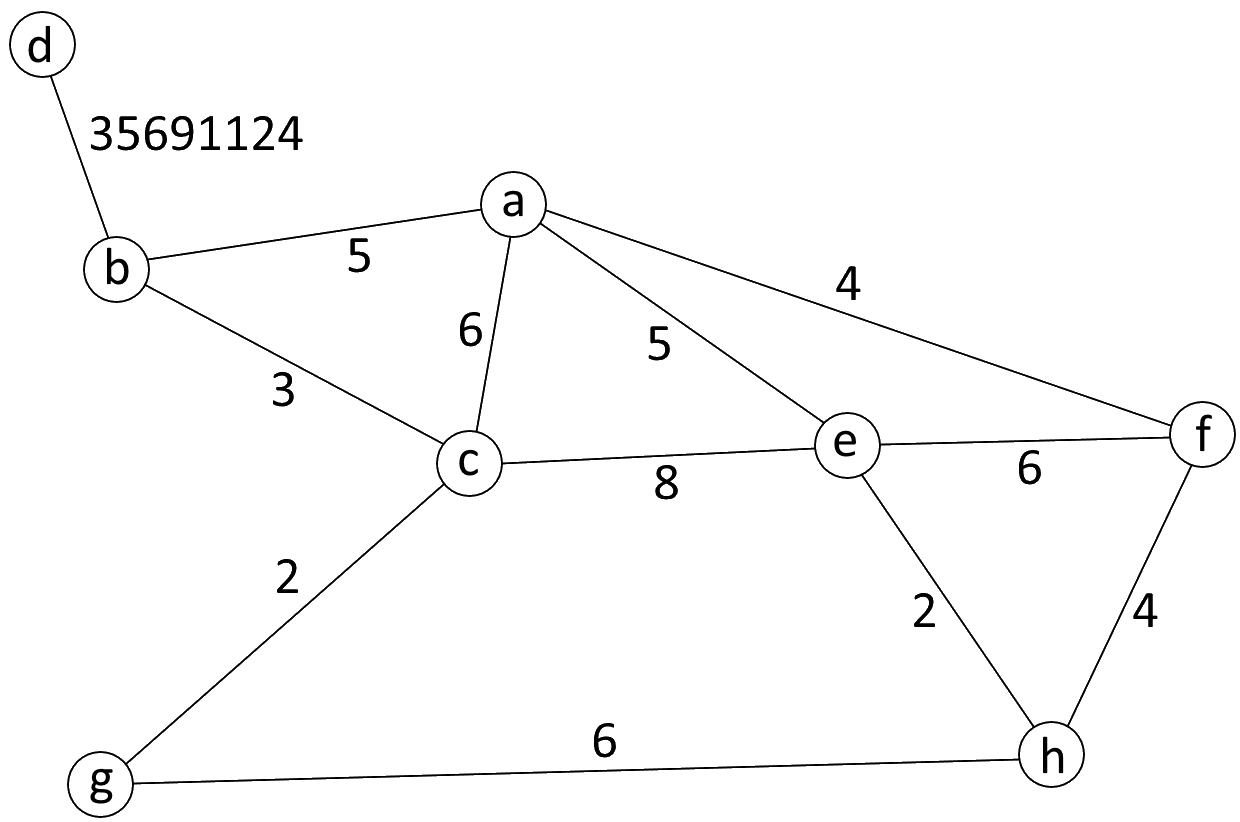
\includegraphics[height=6cm]{scharfhinsehen}
	\end{figure}
\end{frame}

\begin{frame}{Spannbäume}
	\underline{Lösung zu Aufgabe 1} \\
	\forcenewline
	\begin{figure}[htp]
		\centering
		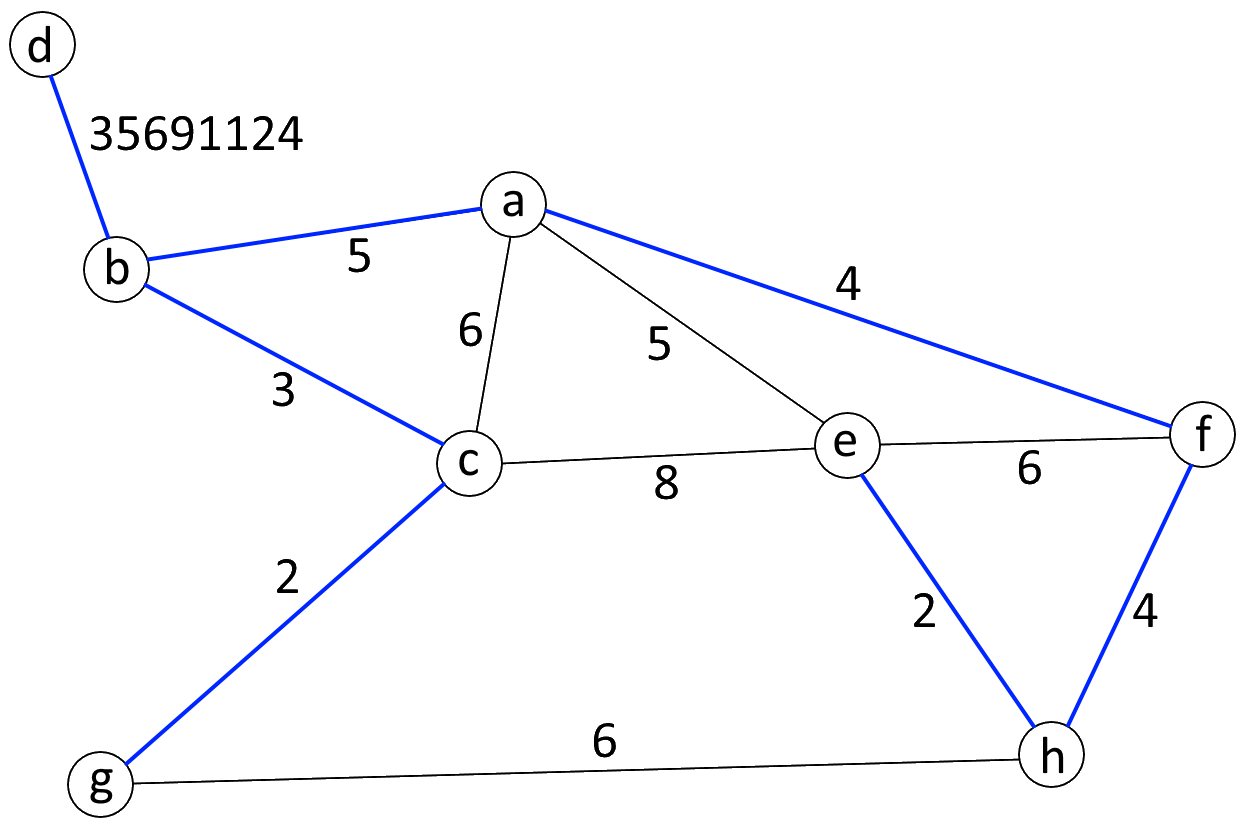
\includegraphics[height=6cm]{scharfhinsehensolution}
	\end{figure}
\end{frame}

\begin{frame}{Spannbäume} %TODO: Maybe {u,v} \in E | u \in S, v \in V\S ?
	\textbf{Die Schnitteigenschaft („Cut Property“)} 
	\begin{itemize}
		\item Sei $U\ \dot{\cup}\ W = V$ irgendeine „Aufteilung“ von $V$ und $C = \big\lbrace \{u, w\} \in E \bigm| u \in U, w \in W \big\rbrace$ alle „Brücken dazwischen“ (genannt \textbf{Schnitt})
		\pause
		\implitem \textbf{Schnitteigenschaft}: \\ 
		Die \textbf{leichteste} Kante $e \in C$ kann in einem MST verwendet werden.
		\pause 
		\item \textbf{Warum?} \\
		\pause \impl Betrachte MST $T$. $U$ und $W$ in $T$ durch $e$ verbunden? \\
		\impl \textbf{Ja}: \yop \\
		\impl \textbf{Nein}: Dann $U$ und $W$ durch andere Kante $e' \in C$ verbunden, und $e'$ darf \textbf{nicht schwerer} als $e$ sein (sonst \crash $T$ minimal) \impl $e$ und $e'$ \textbf{austauschbar}. \qed
	\end{itemize}
\end{frame}


\begin{frame}{Spannbäume}
	\textbf{Die Kreiseigenschaft („Cycle Property“)} 
	\begin{itemize}
		\item Sei $C \subseteq E$ ein  (beliebiger) Kreis in $G$
		\pause
		\implitem \textbf{Kreiseigenschaft}: \\ 
		Für einen MST $T$ von $G$ wird die \textbf{schwerste} Kante $e \in C$ \textbf{nicht} benötigt.
		\pause 
		\item \textbf{Warum}? \\
		\pause \impl Angenommen, $e \in T$ und dafür \textbf{leichtere Kreiskante} $e' \notin T$: \\
		Durch \textbf{Austausch} von $e$ und $e'$ wird Gewicht von $T$ \textbf{kleiner} \\ 
		\impl \crash $T$ minimal \impl Müssen $e$ rausschmeißen. \qed
	\end{itemize}
\end{frame}


\begin{frame}{Spannbäume – Jarník-Prim}
	\textbf{Ein Algorithmus für MSTs: Jarník-Prim} 
	\begin{itemize}
		\implitem \textbf{Idee}: Schnitteigenschaft irgendwie ausnutzen! \\
		\pause
		1. Starte ab beliebigem $s \in V$, setze $S := \{s\}$ \\
		2. \textbf{Erweitere} Knotenmenge $S$ und Baum $T$ \textbf{schrittweise} um die \textbf{minimale} Verbindungskante zu $\ V \setminus S$
		\pause
		\item Schnittkantenmenge $C$ zwischen $S$ und $V \setminus S$ \\
		\impl Verwalte sie in einer \textbf{PriorityQueue} $PQ$
		\pause
		\item[\yop] Funktioniert dank Schnitteigenschaft
	\end{itemize}
\end{frame}

\begin{frame}{Spannbäume – Jarník-Prim}
	\vspace{-.4\baselineskip}
	\begin{exampleblock}{}
		\vspace{-.4\baselineskip}
		\begin{algorithm}[H]
			\small							
			\Function {Jarník-Prim$(G = (V, E))$ \RComment{sieht aus wie Dijkstra}} {
				$\KwSty{pick any } s \in V$\;
				$d := (\infty, ..., \infty) : \KwArray[1...n] \KwOf \R$  \RComment{Distanz zu Knotenmenge S, nicht zu $s \in V$!} \;
				$parent := (\bot, ..., \bot) : \KwArray[1...n] \KwOf V$\;
				$PQ = \{s\} : \text{PriorityQueue}$\;
				$parent[s] := s$ \;
				\While{$PQ \neq \emptyset$} {
					$u := PQ.\text{deleteMin}()$, \quad $d[u] := 0$ \;
					\ForEach{$e = \{u, v\} \in E$} {
						\If{$c(e) < d[v]$} {
							$d[v] := c(e)$\;
							$parent[v] := u$\;
							\begin{tabbing}
								\leIf{$v \in PQ$} {
									\=$PQ.\text{decreaseKey}(v)$ \\
								} {
									\>$PQ.\text{insert}(v)$
								} 
							\end{tabbing}
							\vspace{-\baselineskip}
						}
					}
				}
			\KwRet{$\big\lbrace\,(parent[v],\, v) \mid s \neq v \in V \,\big\rbrace$}\;
			}
		\end{algorithm}
	\end{exampleblock}
\end{frame}

\begin{frame}{Spannbäume – Beispiel Jarník-Prim}
	\centering
	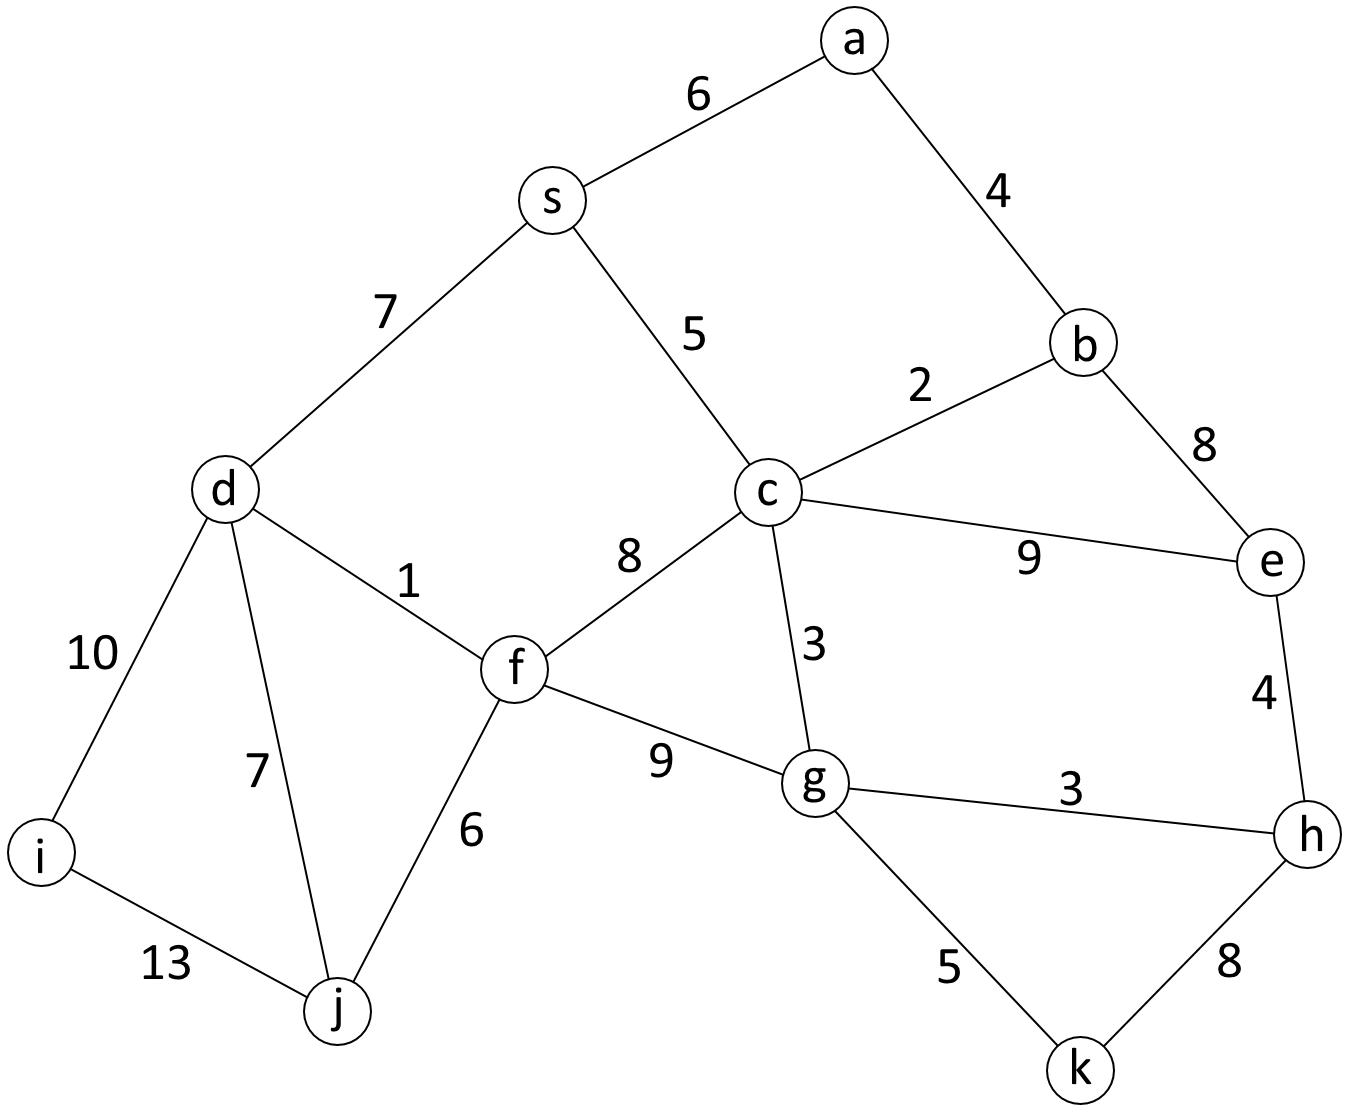
\includegraphics[width=.75\textwidth]{beispielgraph} \\
	\vspace{-.3\baselineskip}\hyperlink{label:afterEx1}{Hier klicken, um das Beispiel zu überspringen.}
\end{frame}

\begin{frame}{Spannbäume – Beispiel Jarník-Prim}
	
		\centering
		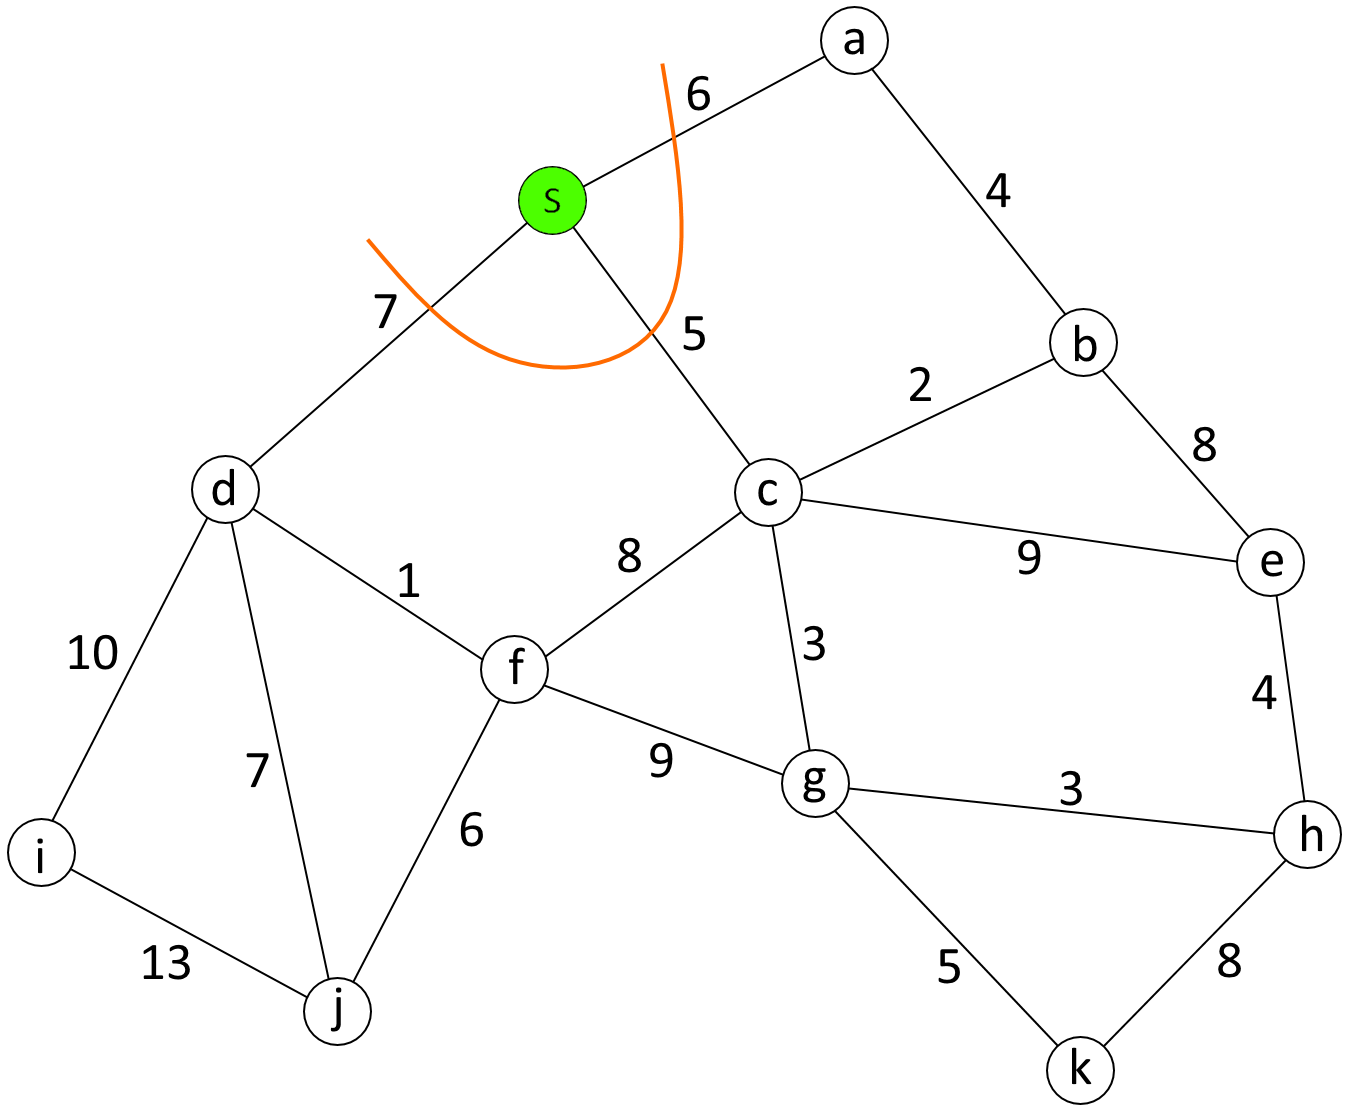
\includegraphics[width=.75\textwidth]{jp1}
	
\end{frame}

\begin{frame}{Spannbäume – Beispiel Jarník-Prim}
	
		\centering
		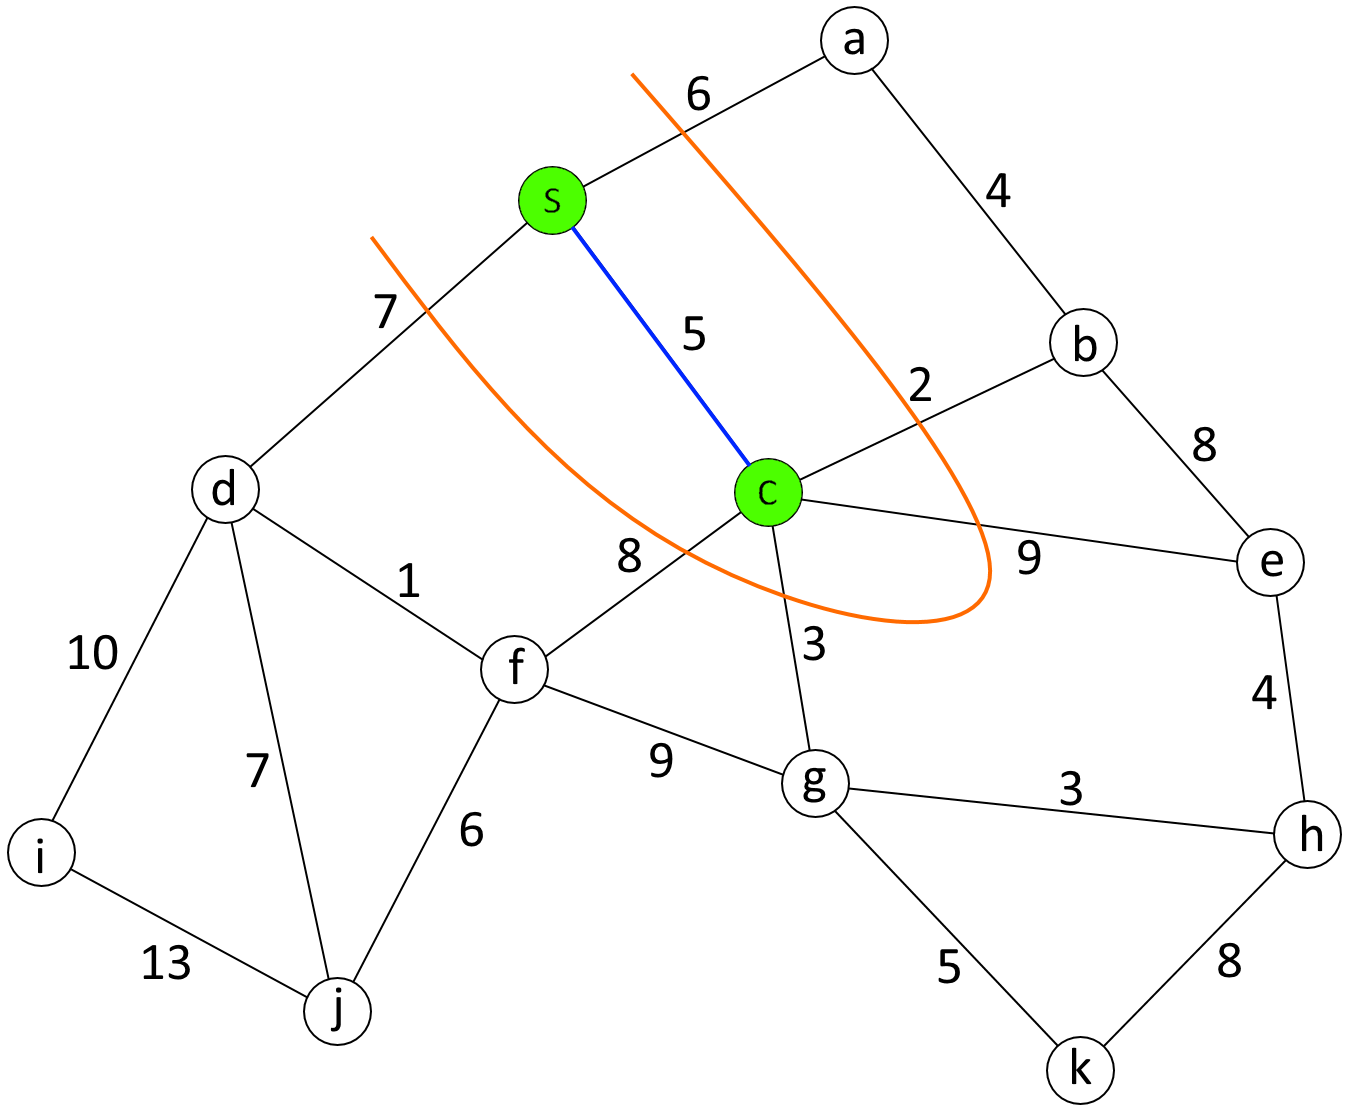
\includegraphics[width=.75\textwidth]{jp2}
	
\end{frame}

\begin{frame}{Spannbäume – Beispiel Jarník-Prim}
	
		\centering
		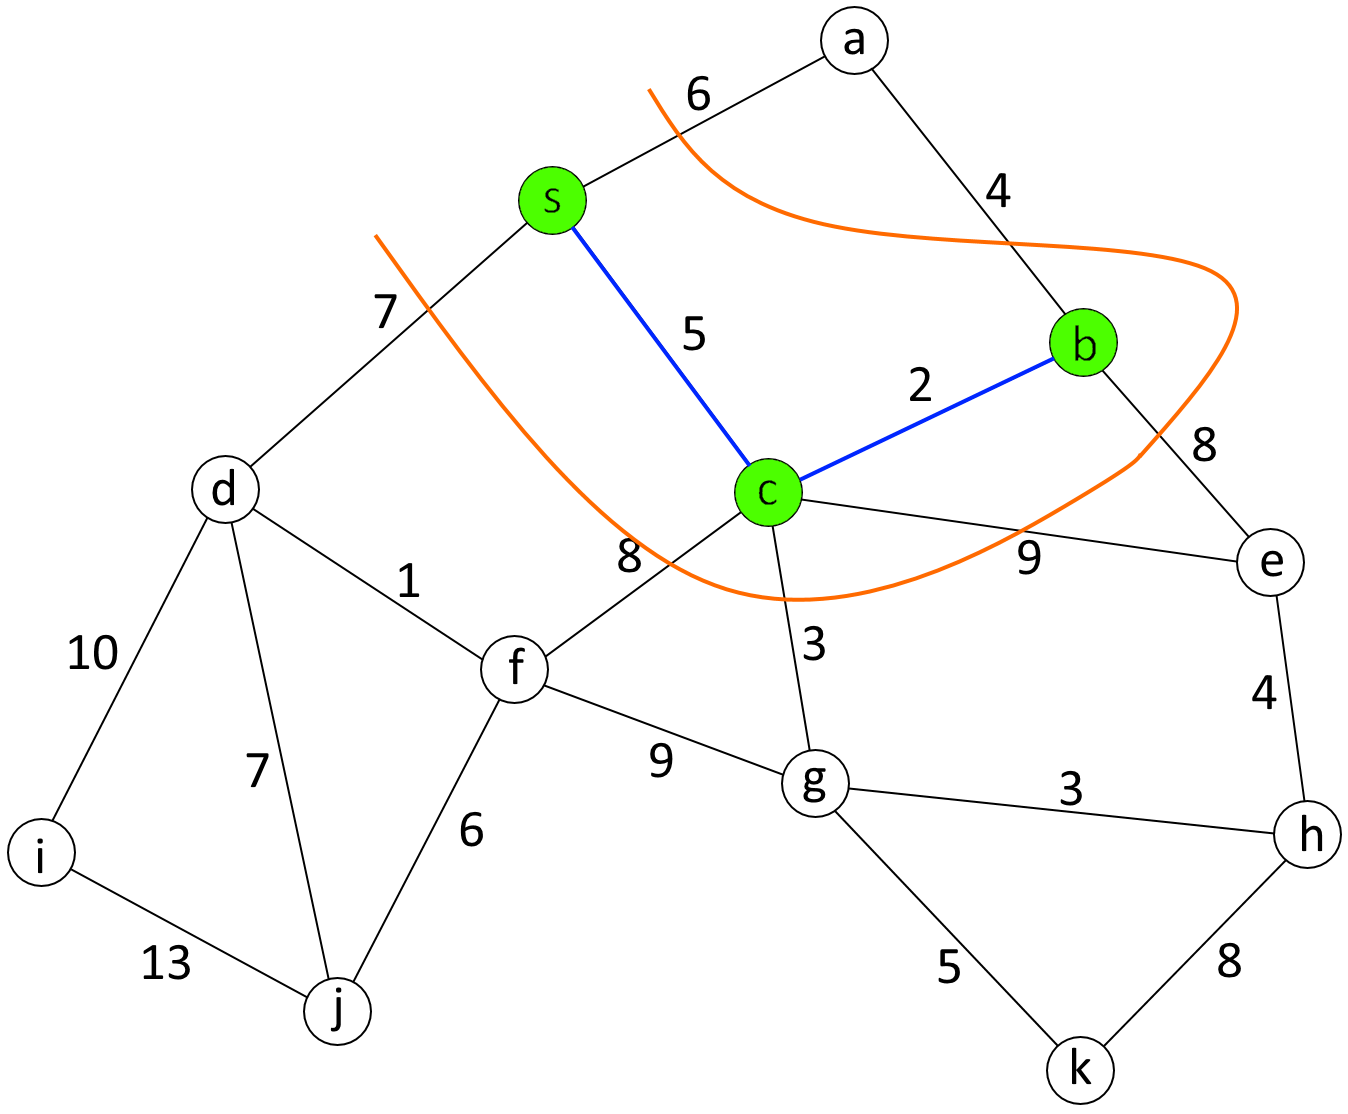
\includegraphics[width=.75\textwidth]{jp3}
	
\end{frame}

\begin{frame}{Spannbäume – Beispiel Jarník-Prim}
	
		\centering
		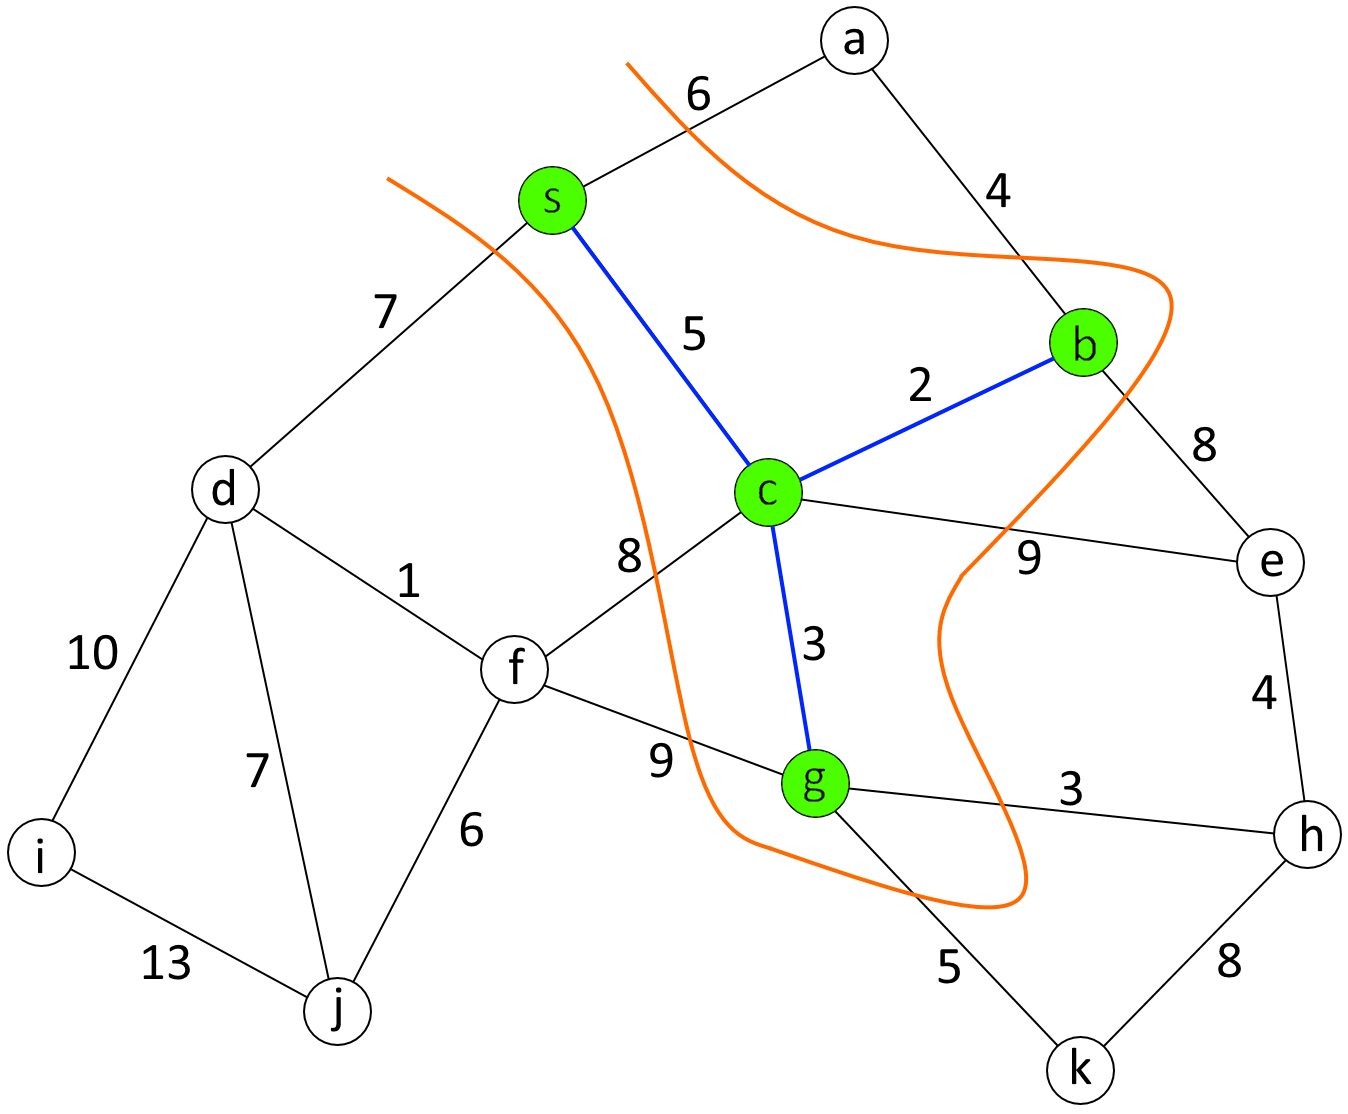
\includegraphics[width=.75\textwidth]{jp4}
	
\end{frame}

\begin{frame}{Spannbäume – Beispiel Jarník-Prim}
	
		\centering
		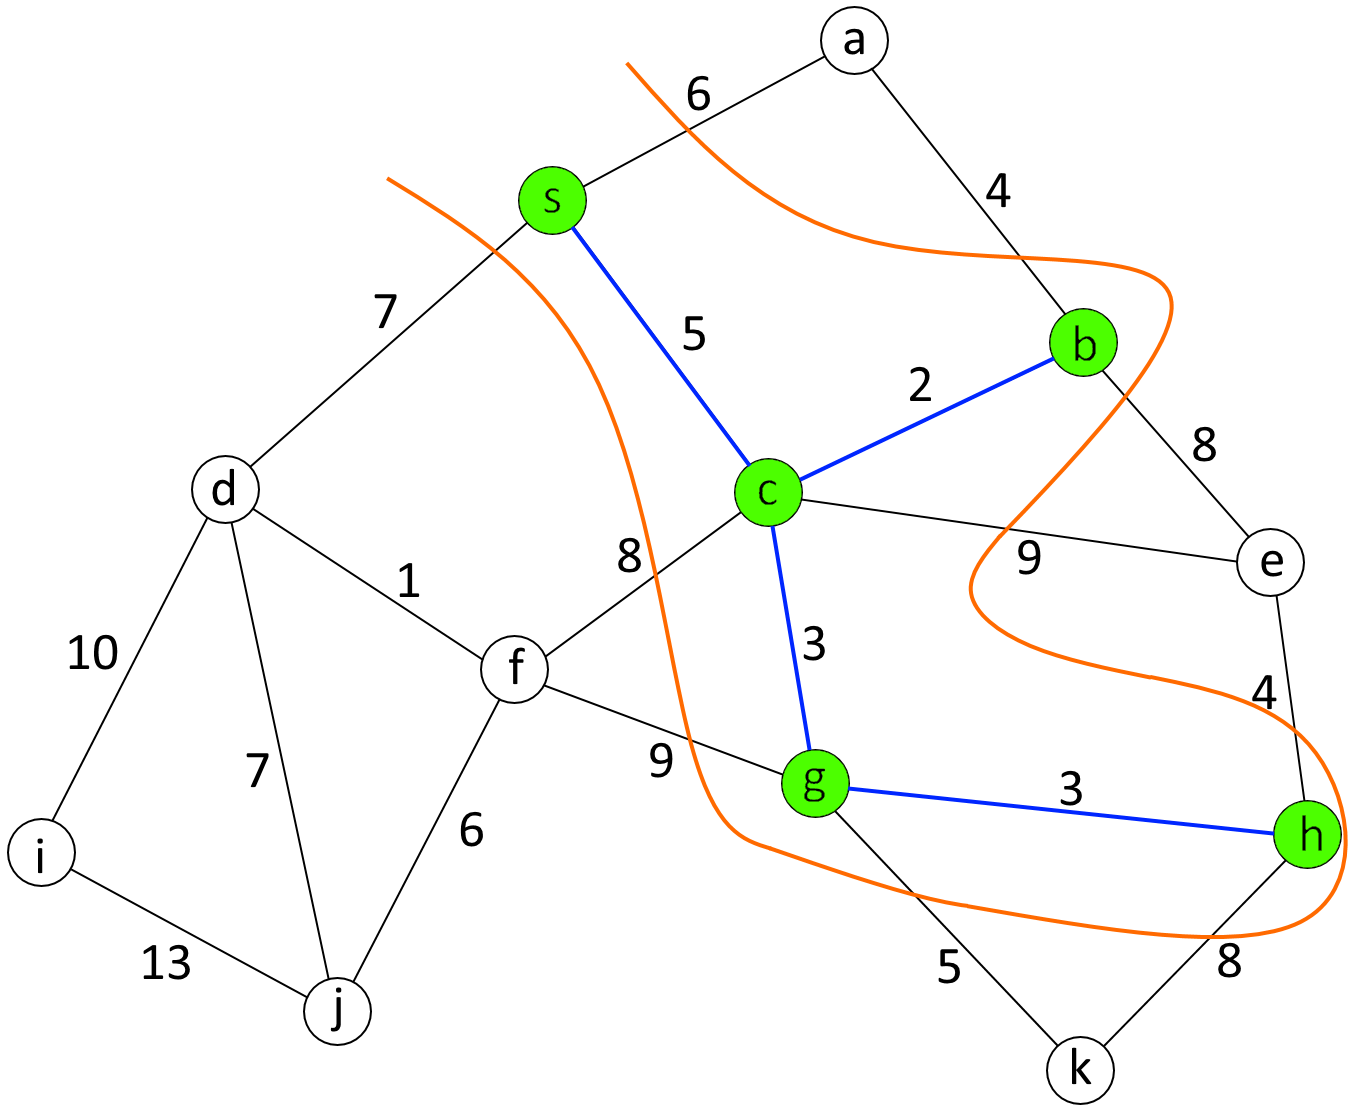
\includegraphics[width=.75\textwidth]{jp5}
	
\end{frame}

\begin{frame}{Spannbäume – Beispiel Jarník-Prim}
	
		\centering
		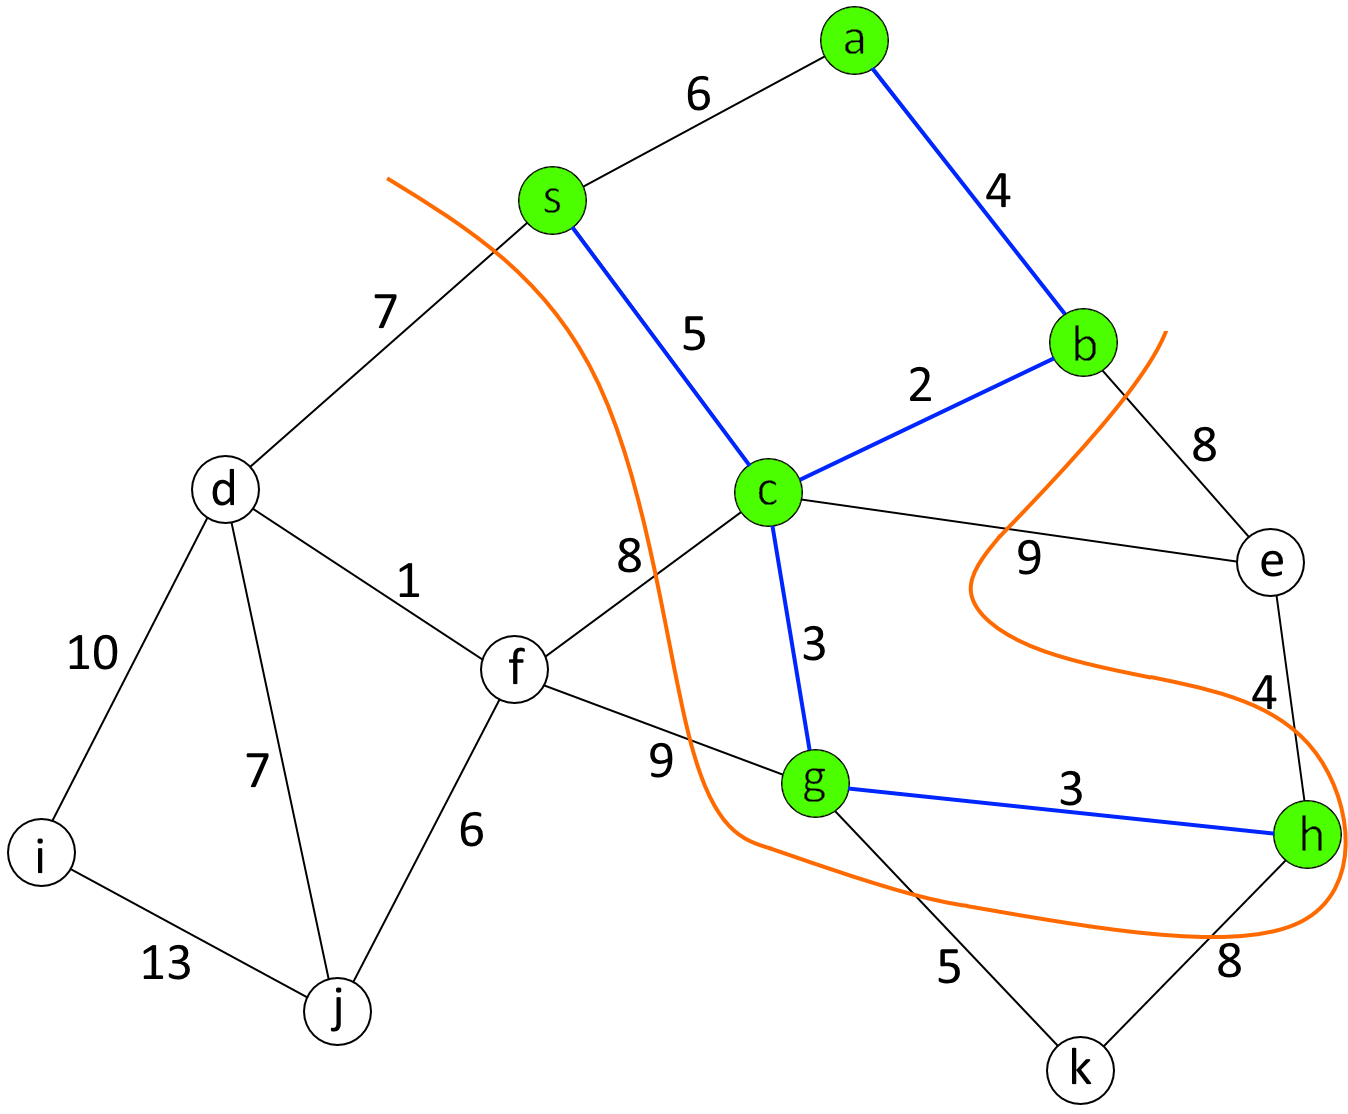
\includegraphics[width=.75\textwidth]{jp6}
	
\end{frame}

\begin{frame}{Spannbäume – Beispiel Jarník-Prim}
	
		\centering
		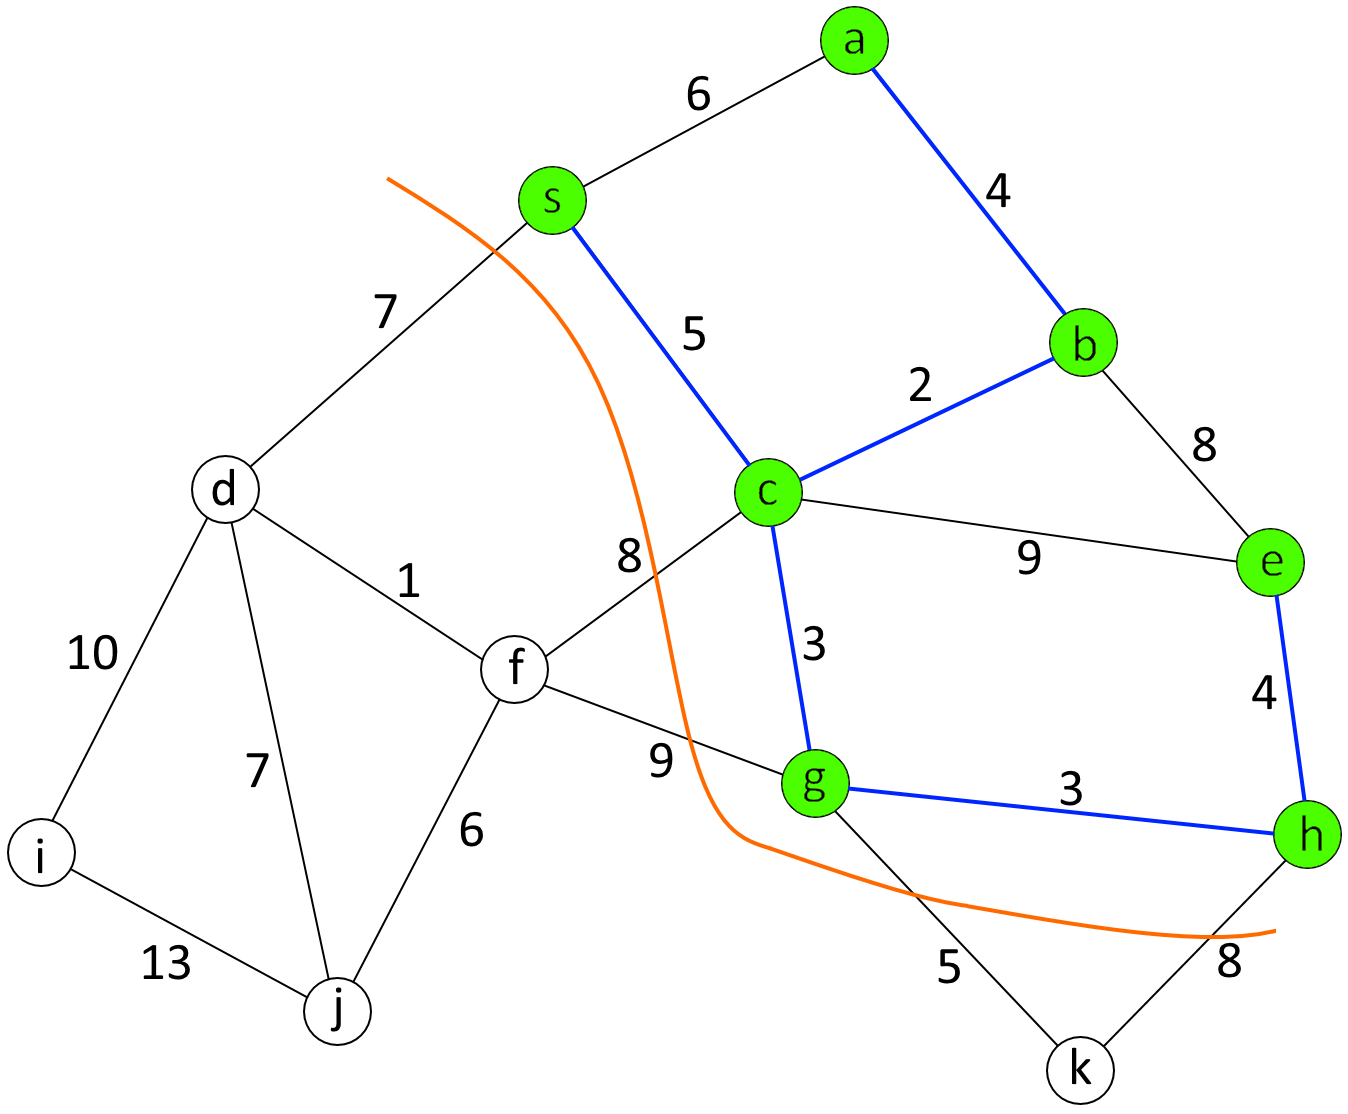
\includegraphics[width=.75\textwidth]{jp7}
	
\end{frame}

\begin{frame}{Spannbäume – Beispiel Jarník-Prim}
	
		\centering
		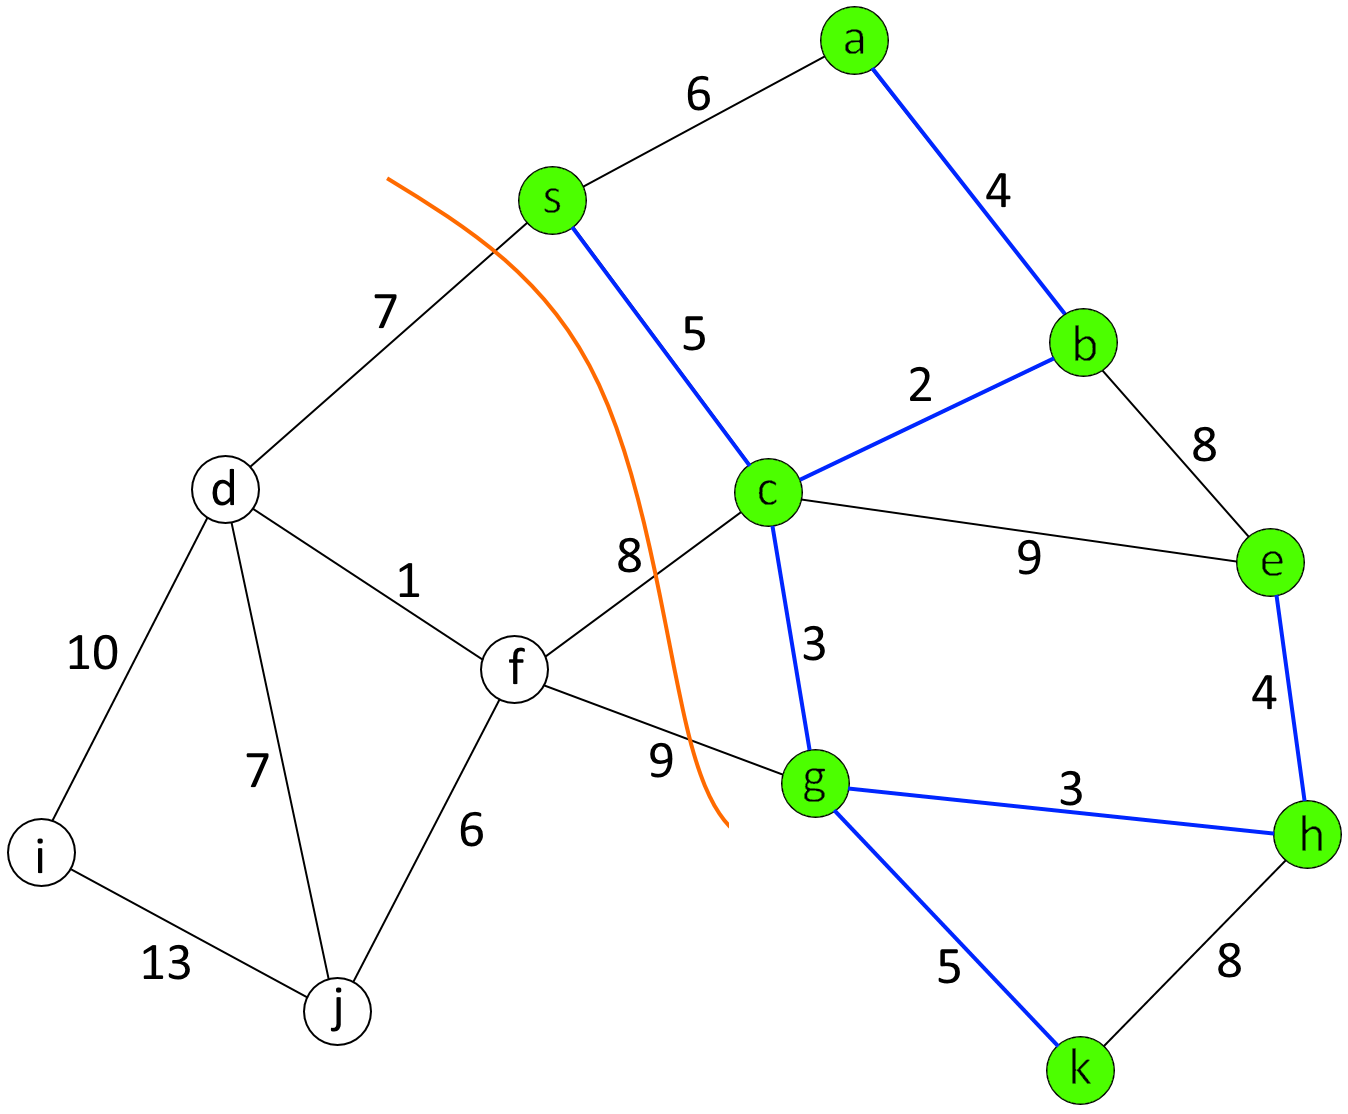
\includegraphics[width=.75\textwidth]{jp8}
	
\end{frame}

\begin{frame}{Spannbäume – Beispiel Jarník-Prim}
	
		\centering
		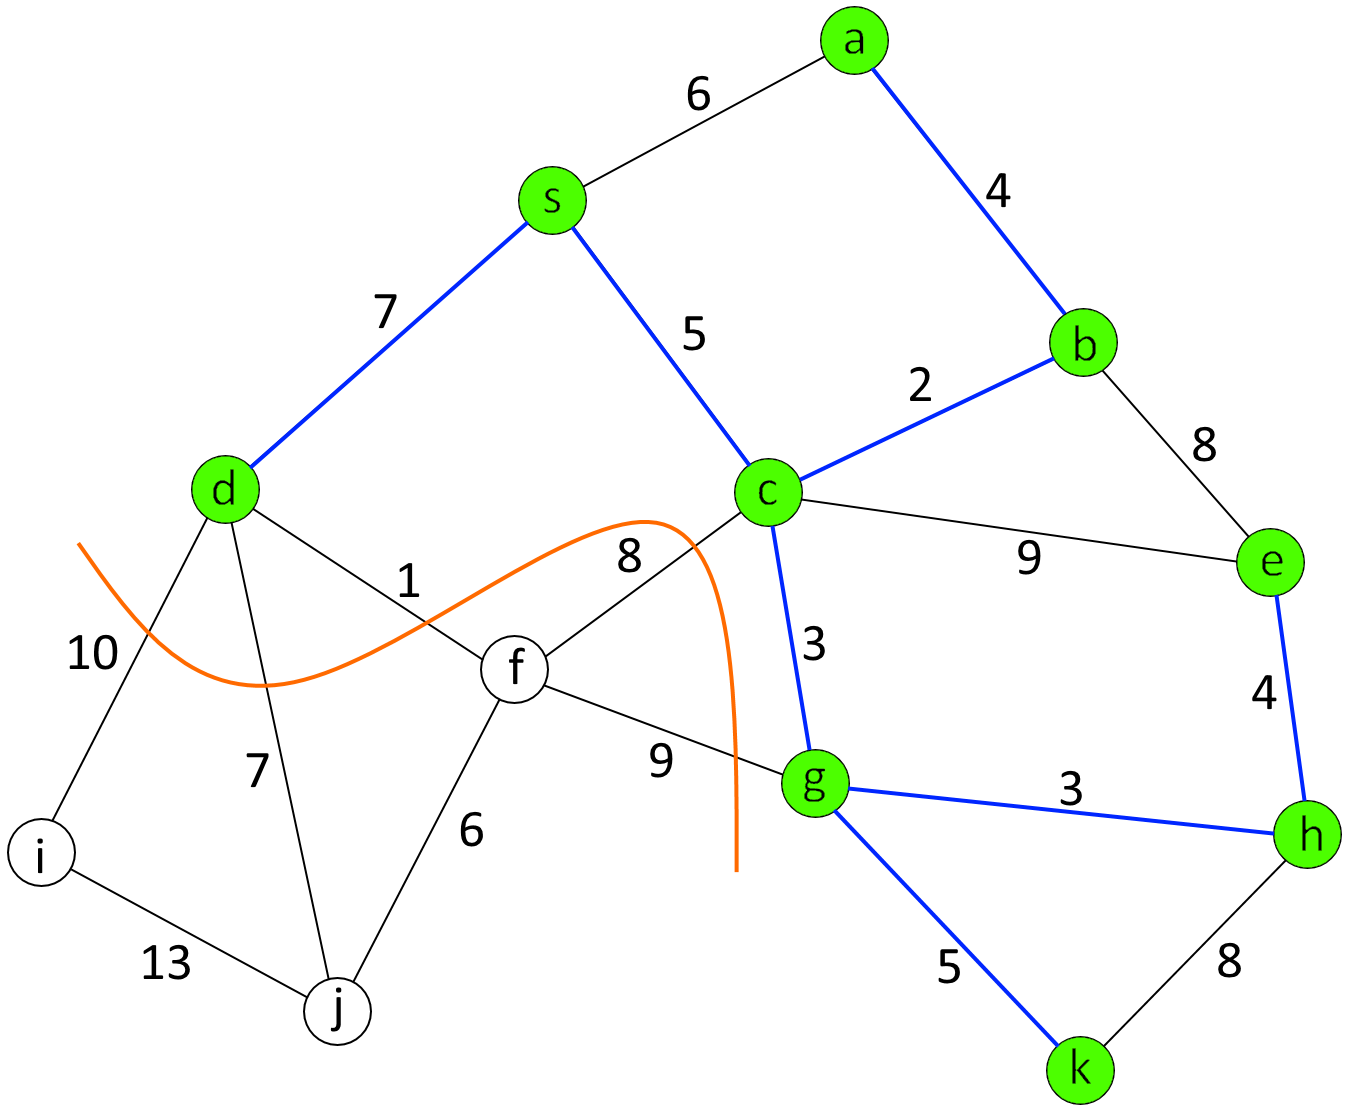
\includegraphics[width=.75\textwidth]{jp9}
	
\end{frame}

\begin{frame}{Spannbäume – Beispiel Jarník-Prim}
	
		\centering
		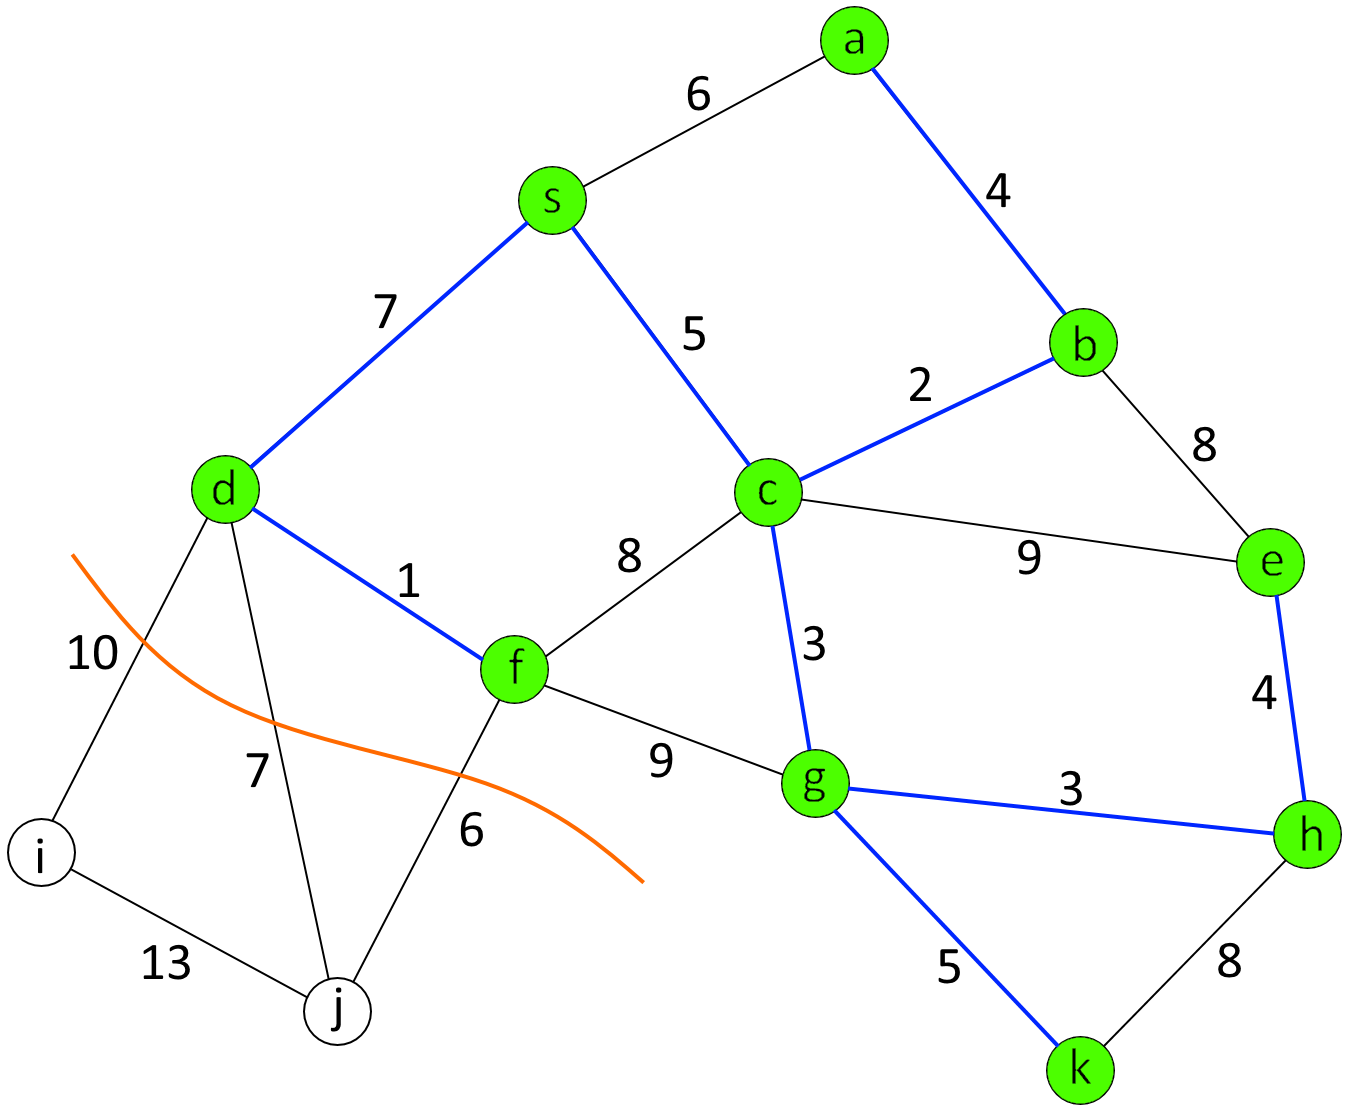
\includegraphics[width=.75\textwidth]{jp10}
	
\end{frame}

\begin{frame}{Spannbäume – Beispiel Jarník-Prim}
	
		\centering
		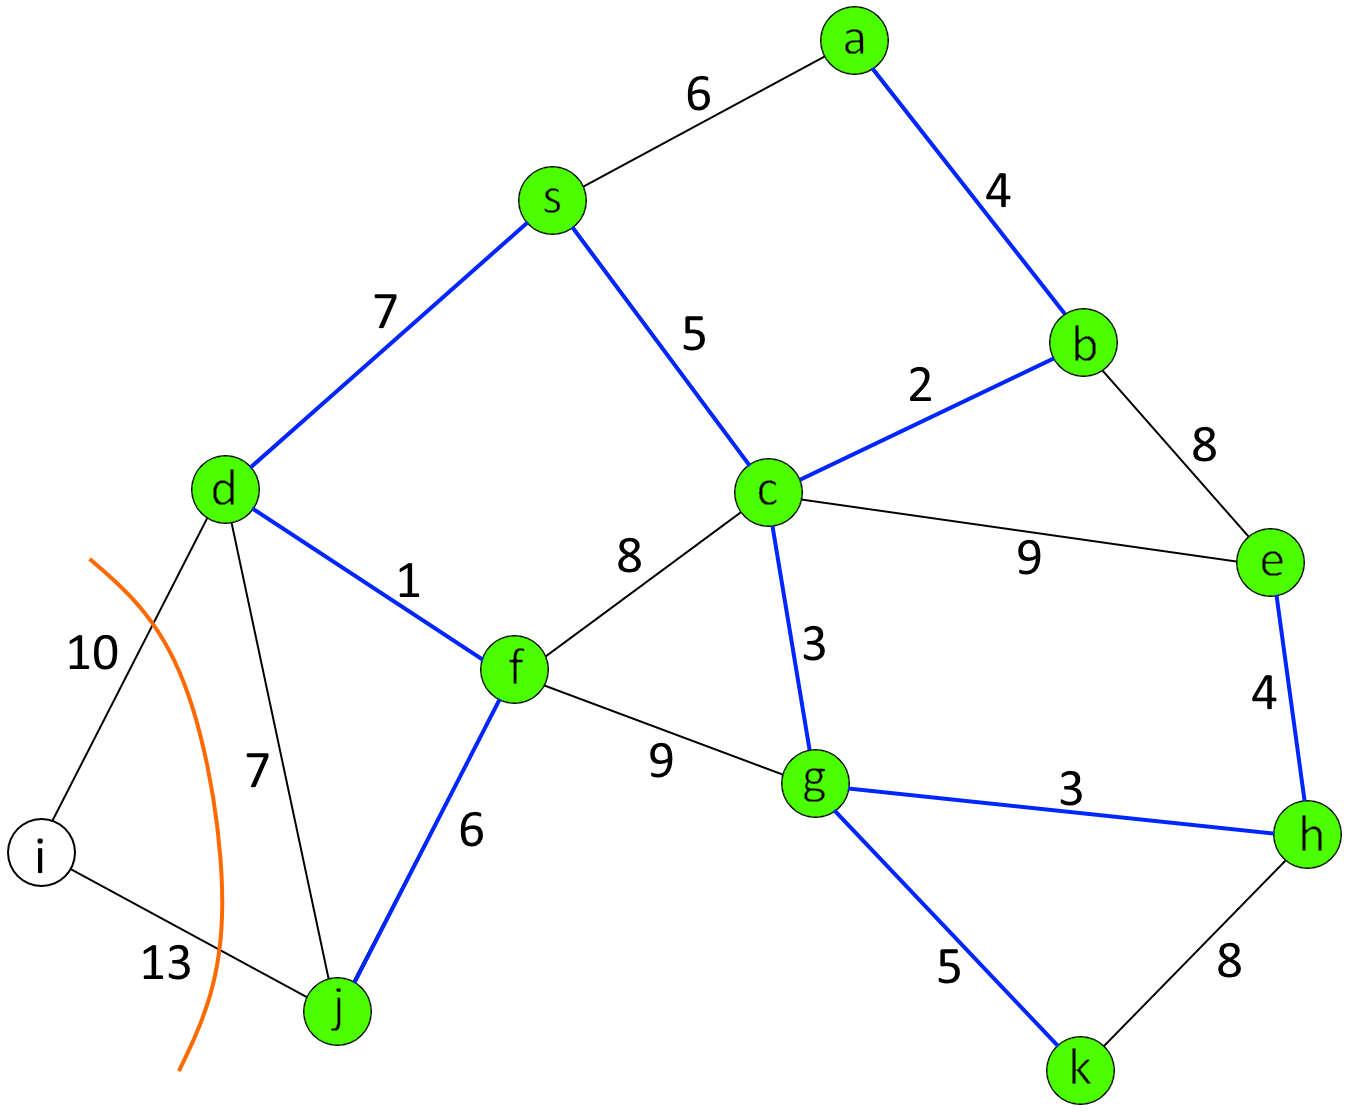
\includegraphics[width=.75\textwidth]{jp11}
	
\end{frame}

\begin{frame}{{\hypertarget{label:afterEx1}{}Spannbäume – Beispiel Jarník-Prim}}
		\centering
		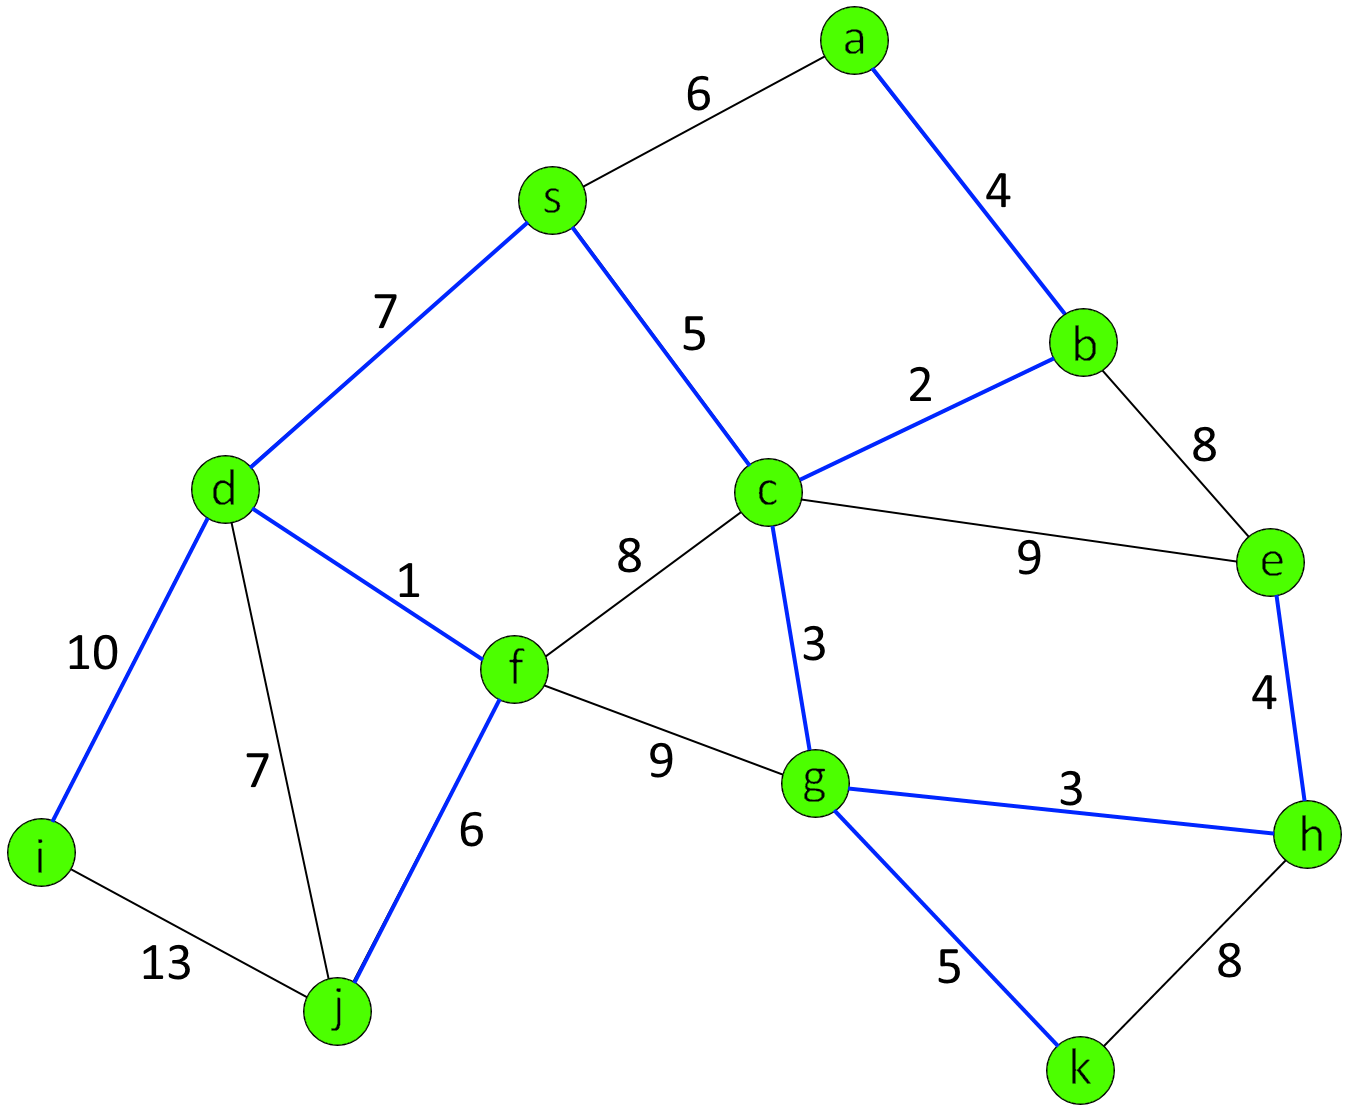
\includegraphics[width=.75\textwidth]{jp12}
\end{frame}

\begin{frame}{Spannbäume – Jarník-Prim}
	\textbf{Laufzeit von Jarník-Prim: same as Dijkstra} 
	\begin{itemize}
		\item[] Im Worst-Case $m$-mal $decreaseKey$
		\item[$+$] Genau $n$-mal $deleteMin$ und $insert$
		\pause
		\item[$=$] Mit binärem Heap: $O\left((m+n)\log n\right)$
		\pause
		\item[$=$] Mit Fibonacci-Heap: $O(m + n \log n)$ \quad (amortisiert und mit höheren konstanten Faktoren)
	\end{itemize}
\end{frame}

\begin{frame}{Spannbäume – Kruskal}
	\textbf{Rosinen rauspicken mit Kruskal} 
	\begin{itemize}
		\item \textbf{Idee}: Baum (bzw. Wald) \textbf{schrittweise} \textbf{wachsen} lassen 
		\pause
		\implitem Durchlaufe \textbf{Kanten} nach \textbf{aufsteigendem} Gewicht: \\
		Nehme Kante zum Wald \textbf{dazu}, falls dadurch \textbf{kein Kreis} entsteht \\
		{\small (also wenn die Kante \textbf{zwei separate} Bäume vereinigt)}
		\pause
		\item Am \textbf{Ende}: Alle ausgewählten Kanten ergeben einen MST
		\pause
		\item[\yop] Funktioniert dank Schnitt- und Kreiseigenschaft
	\end{itemize}
	\pause
	\forcenewline
	\textbf{Wollen dafür effizient}...
	\begin{itemize}
		\item ...heraus\textbf{finden}, zu welcher Menge ein Element gehört ($find$)
		\item ...die Mengen zweier Elemente \textbf{vereinigen} ($union$)
	\end{itemize}
\end{frame}

\begin{frame}{Union-Find}
	\textbf{\impl Eine neue Datenstruktur!} \\
	Fürs Grobe...
	\begin{itemize}
		\item Repräsentiere Menge $M \subseteq \{1...n\}$ durch \textbf{beliebiges} Element $w \in M$
		\pause
		\item Intern: $M$ wird als \textbf{Baum}, $w$ als \textbf{Wurzel} von $M$ behandelt
		\pause
		\implitem Verwalte $parent: \KwArray[1...n] \KwOf 1...n$, \ wobei \\
		$parent[v] = v \gdw v$ ist Wurzel \\ Am \textbf{Anfang}: $parent[v] := v$ \RComment{Alle Elemente sind eigene Wurzel} \\
		\visible<3->{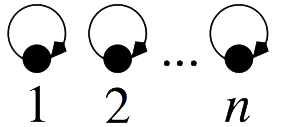
\includegraphics[width=.2\textwidth]{init}}
	\end{itemize}
	\pause
	...und für die Effizienz
	\begin{itemize}
		\implitem Verwalte $rank = (0,...,0) : \KwArray[1...n] \KwOf 0 ...\log n$, \ wobei \\
		$rank[v] = \casesl{
			\begin{varwidth}{\linewidth} Höhe von Baum von $v$ \vspace{-.13\baselineskip} \\ \footnotesize (ohne Pfadkompression) \end{varwidth},
				& \text{$v$ ist Wurzel} \\
			\textit{garbage}, 
				& \text{$v$ ist \textbf{keine} Wurzel}}$
		%\item Für eine \textbf{Wurzel} $w \in M$ ist $rank[w]$ die \textbf{maximal mögliche} Länge des \textbf{längsten} Pfades von einem Element $e \in M$ zu $w$
	\end{itemize}
\end{frame}

\begin{frame}{Union-Find – Operationen}
	\begin{exampleblock}{Finden}
		\begin{columns}[T] 
			\begin{column}[T]{.5\linewidth} 
				\begin{algorithm}[H]
					\Function {find$(e : 1..n) : 1..n$} {
						\eIf{$parent[e] = e$} {
							\KwRet{$e$}\;
						} {
							$w := \text{find}(parent[e])$\;
							\LComment{Pfadkompression} \;
							$parent[e] := w$\;
							\KwRet{$w$}\;
						}
					}
				\end{algorithm}
			\end{column}
			\begin{column}[T]{.4\linewidth} 
				\bigskip
				\begin{figure}[b]
					\centering
					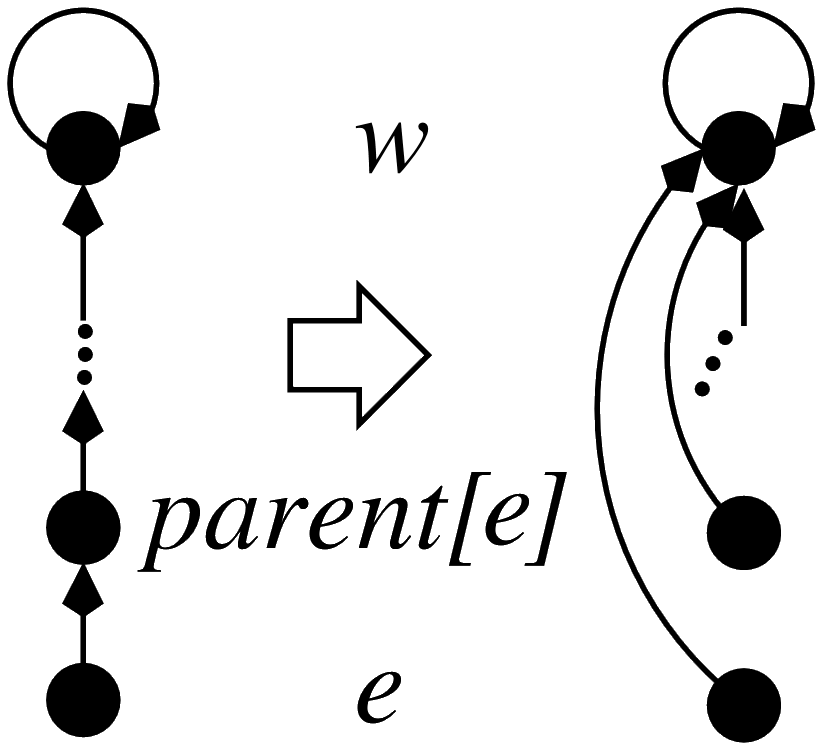
\includegraphics[width=.7\textwidth]{pfadkompression}
					\caption{Pfadkompression}
				\end{figure}
			\end{column}
		\end{columns}
	\end{exampleblock}
\end{frame}

\begin{frame}{Union-Find – Operationen}
	\begin{exampleblock}{Vereinigen}
		\begin{columns}[T] 
			\begin{column}[T]{.5\linewidth} 
				\begin{algorithm}[H]
	
					\Procedure {union$(a', b' : 1...n)$} {
						$\Matrix{a \\ b} := \Matrix{\text{find}(a') \\ \text{find}(b')}$ \;
						\If{$a \neq b$} {
							\LComment{union by rank} \;
							\eIf{$rank[a] < rank[b]$} {
								$parent[a] := b$\;
							} {
								$parent[b] := a$\;
								\If{$rank[a] = rank[b]$} {
									$rank[a]\pp$\;
								}
							}
						}
					}
				\end{algorithm}
			\end{column}
			\begin{column}[T]{.4\linewidth} 
				\vspace{5\bigskipamount}
				\begin{figure}[b]
					\centering
					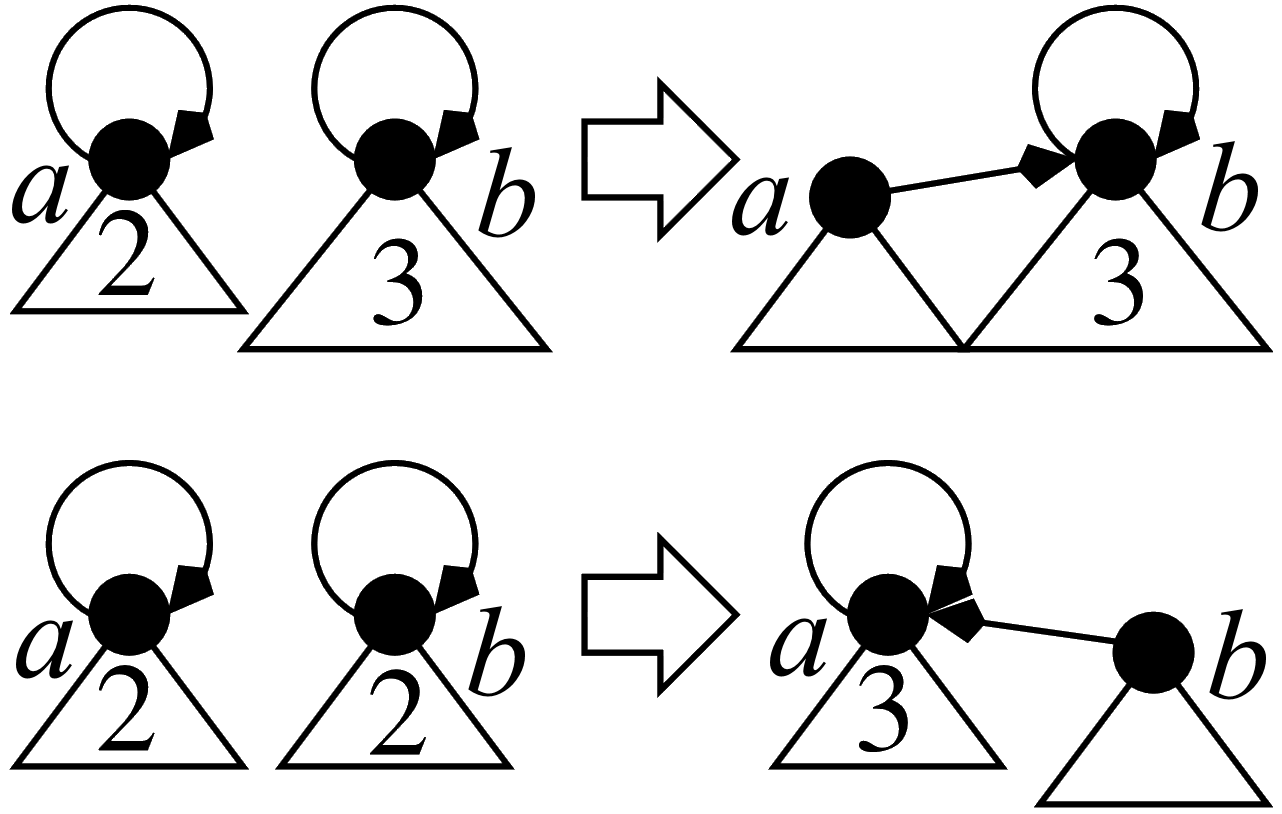
\includegraphics[width=\textwidth]{unionbyrank}
					\caption{Union-by-rank}
				\end{figure}
			\end{column}
		\end{columns}
	\end{exampleblock}
\end{frame}


\begin{frame}{Spannbäume – Kruskal}
	\begin{exampleblock}{Kruskal -- Pseudocode}
		\begin{algorithm}[H]
			\Function {Kruskal$(G = (V, E))$} {
				$forest := \KwNew \text{UnionFind}(n)$ \;
				$T := \emptyset$\;
				$\text{Sort}(E) \KwSty{ by } c$ \;
				\ForEach{$e = \{u, v\} \in E$} {
					\If{$forest.\text{find}(u) \neq forest.\text{find}(v)$} {
						$T := T \cup \{e\}$\;
						$forest.\text{union}(u, v)$\;
					}
				}
				\KwRet{$T$}\;
			}
		\end{algorithm}
	\end{exampleblock}
\end{frame}

\begin{frame}{Spannbäume – Beispiel Kruskal}
	\centering
	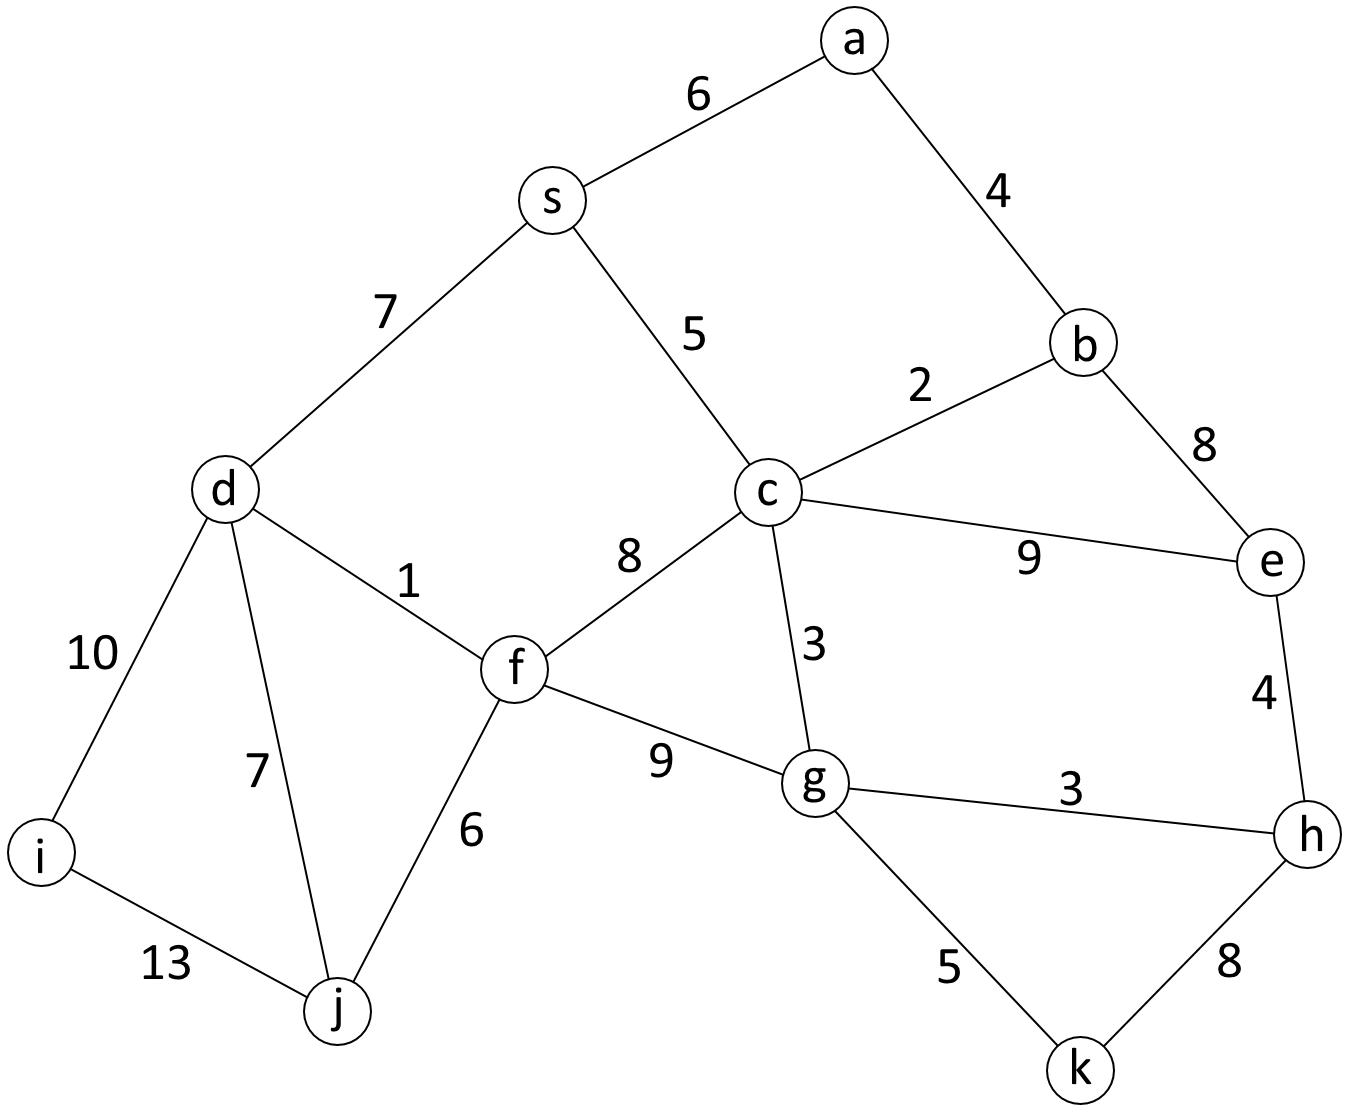
\includegraphics[width=.75\textwidth]{beispielgraph} \\
	\vspace{-.3\baselineskip}\hyperlink{label:afterEx2}{Hier klicken, um das Beispiel zu überspringen.}
\end{frame}

\begin{frame}{Spannbäume – Beispiel Kruskal}
	\centering
	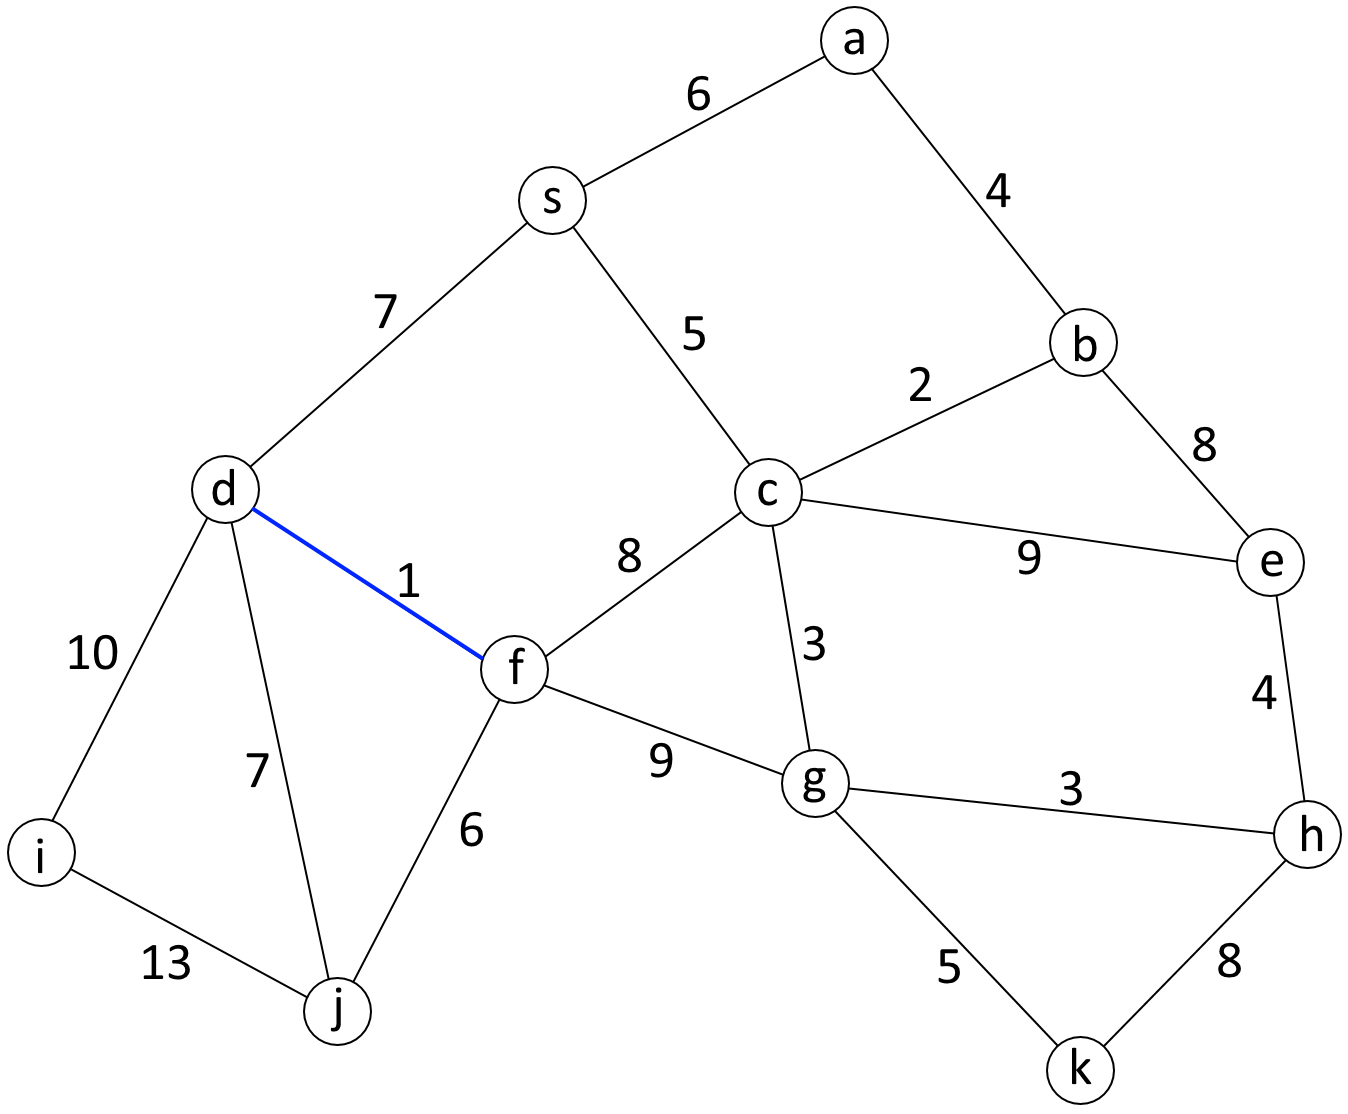
\includegraphics[width=.75\textwidth]{k1}
\end{frame}

\begin{frame}{Spannbäume – Beispiel Kruskal}
	
		\centering
		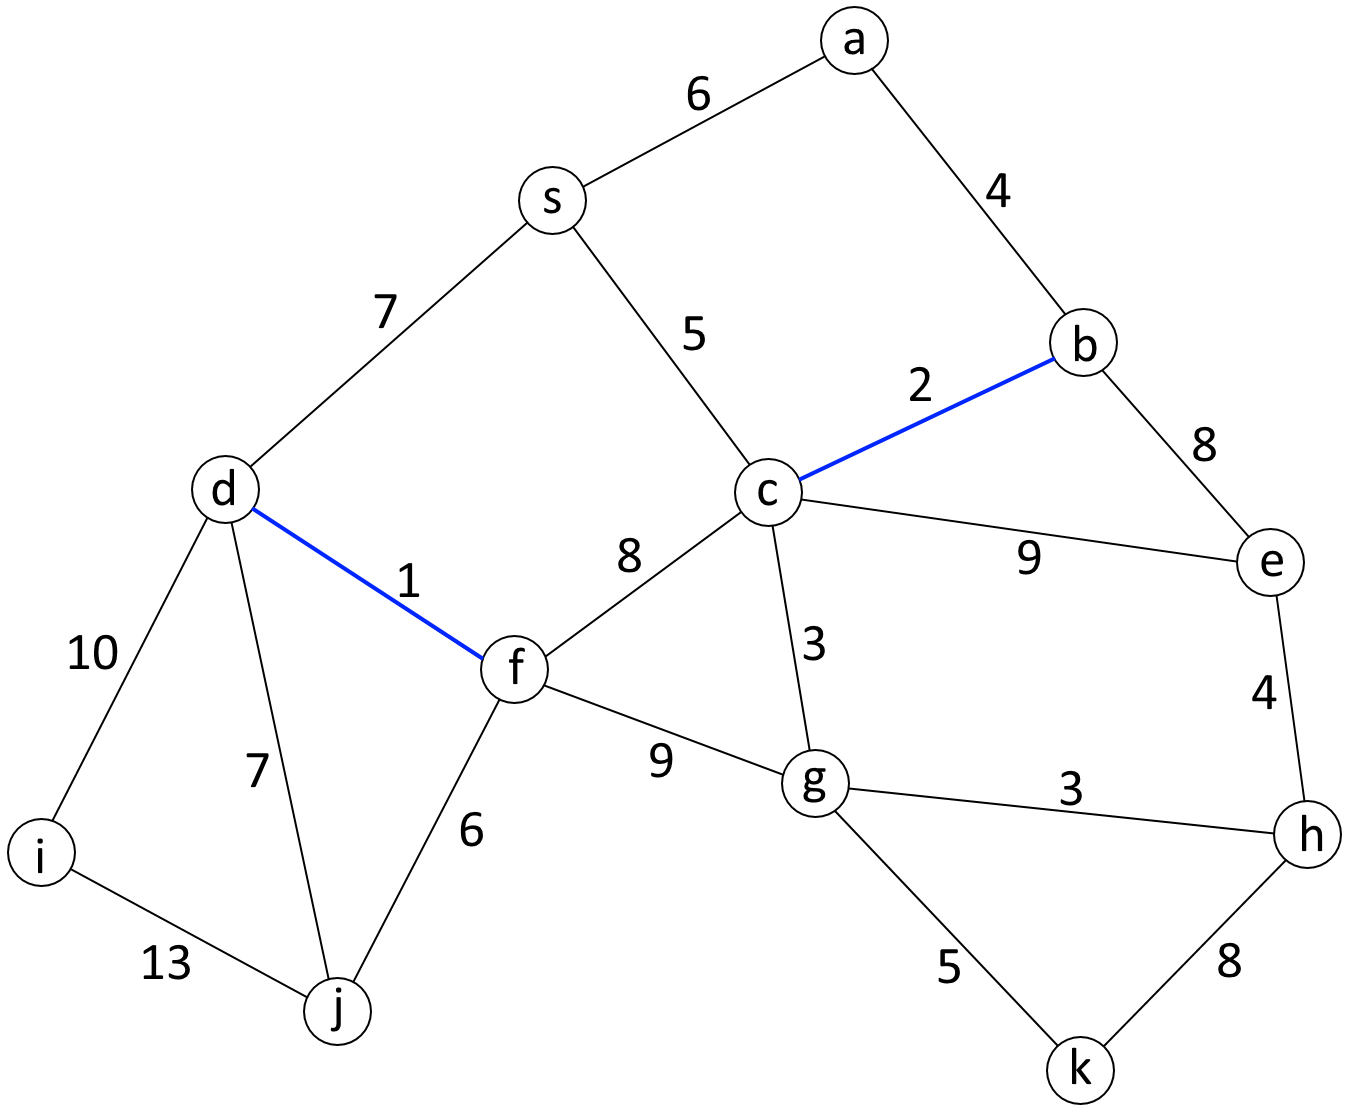
\includegraphics[width=.75\textwidth]{k2}
	
\end{frame}

\begin{frame}{Spannbäume – Beispiel Kruskal}
	
		\centering
		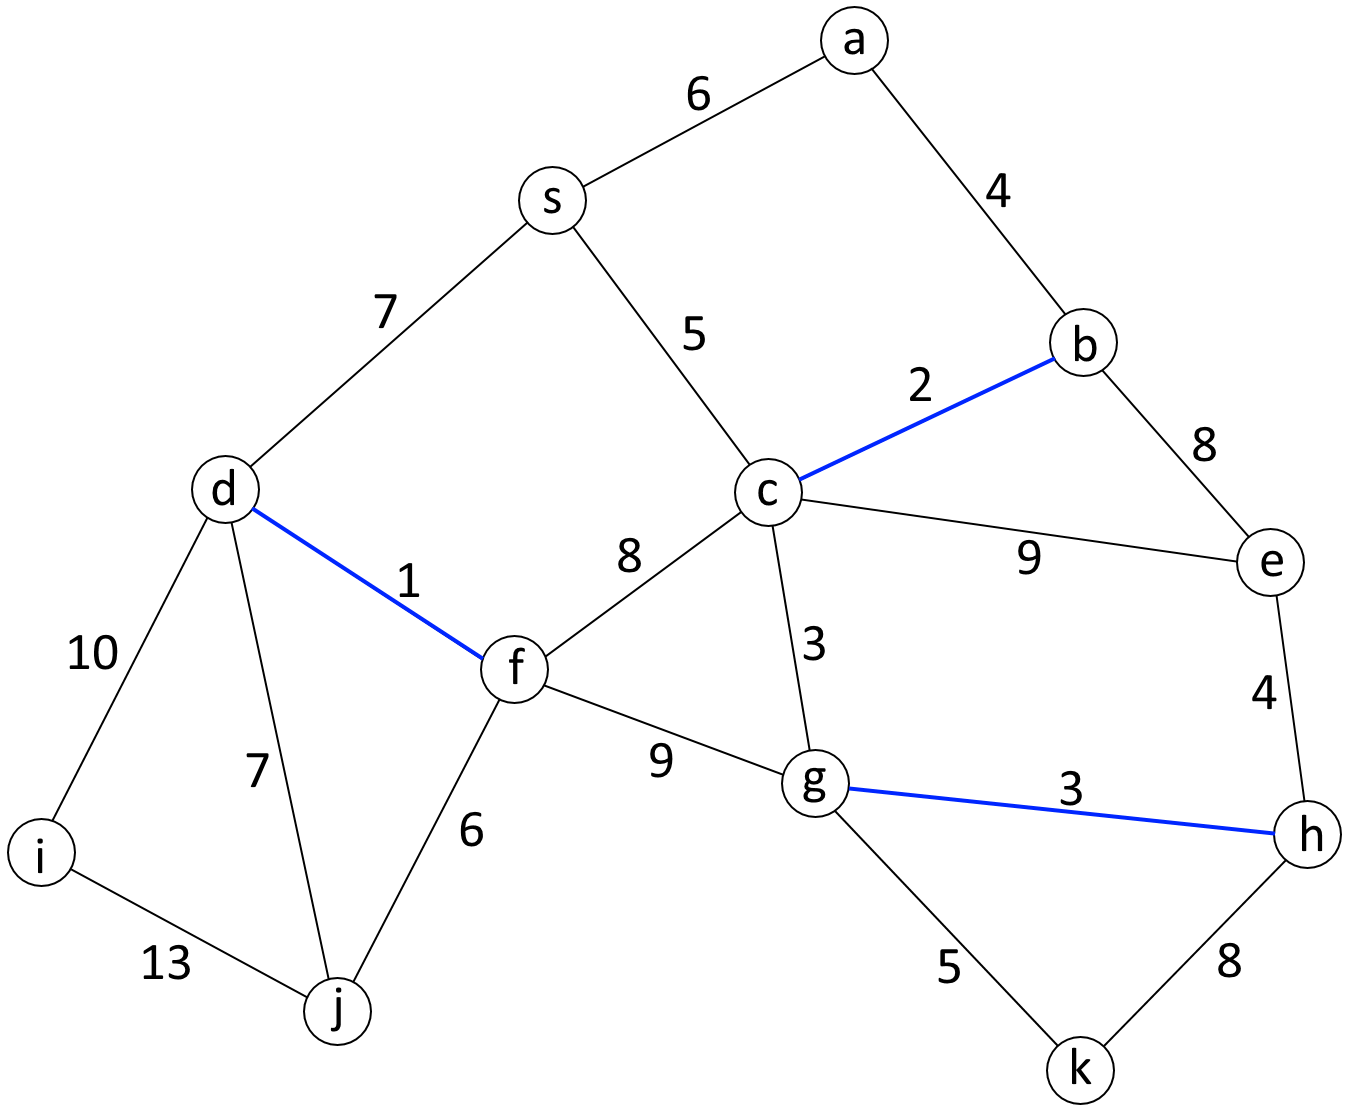
\includegraphics[width=.75\textwidth]{k3}
	
\end{frame}

\begin{frame}{Spannbäume – Beispiel Kruskal}
	
		\centering
		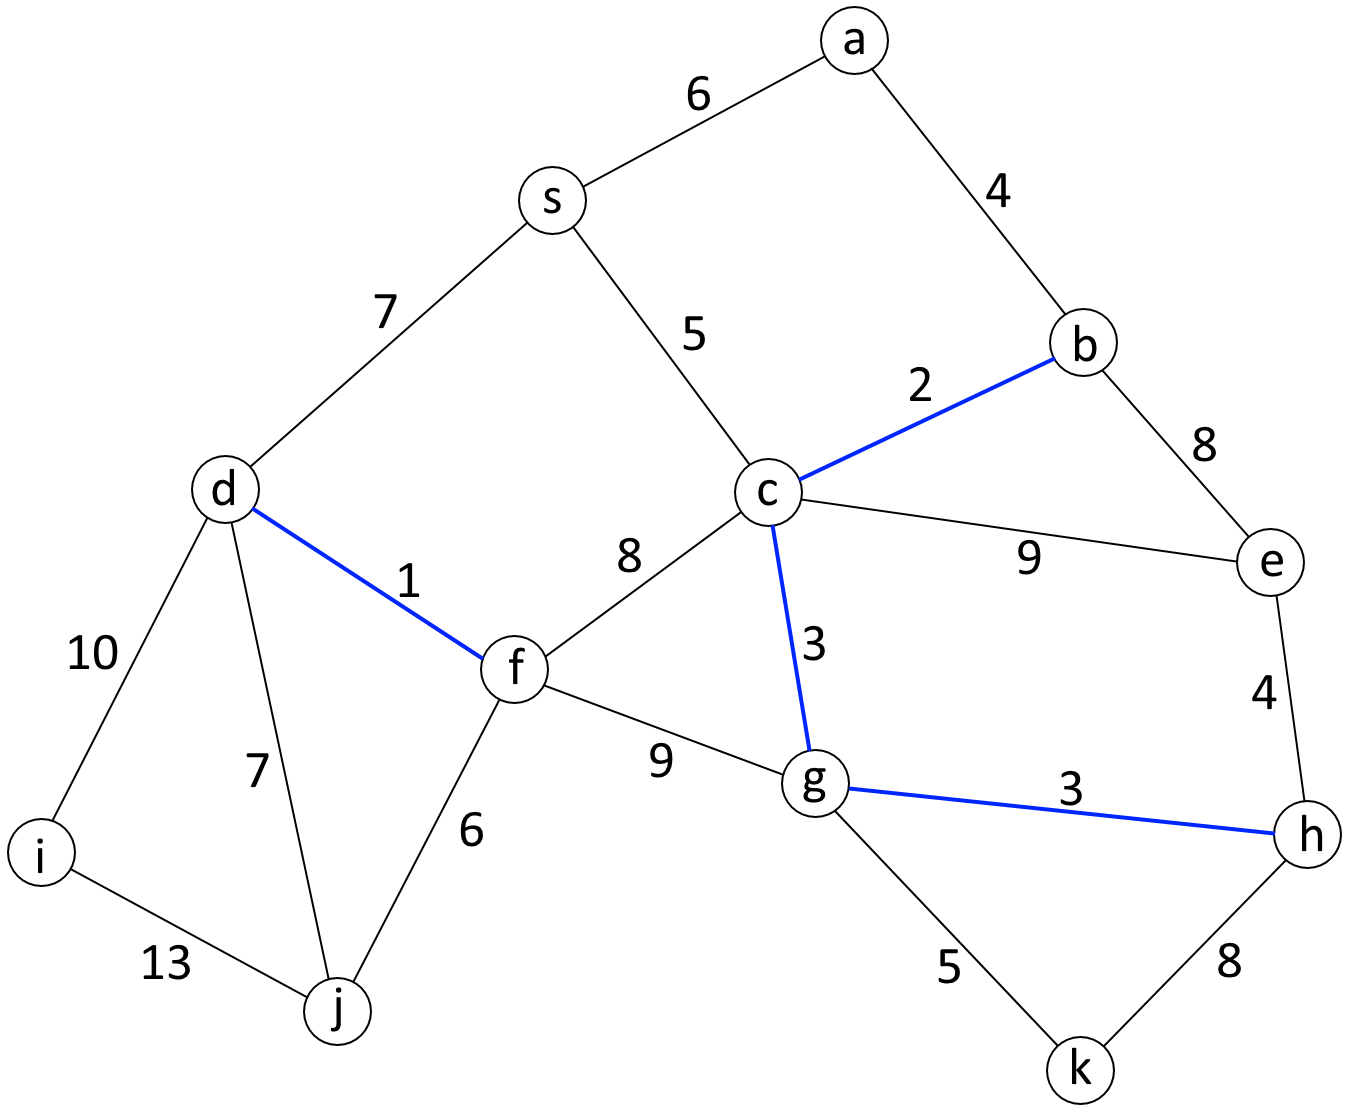
\includegraphics[width=.75\textwidth]{k4}
	
\end{frame}

\begin{frame}{Spannbäume – Beispiel Kruskal}
	
		\centering
		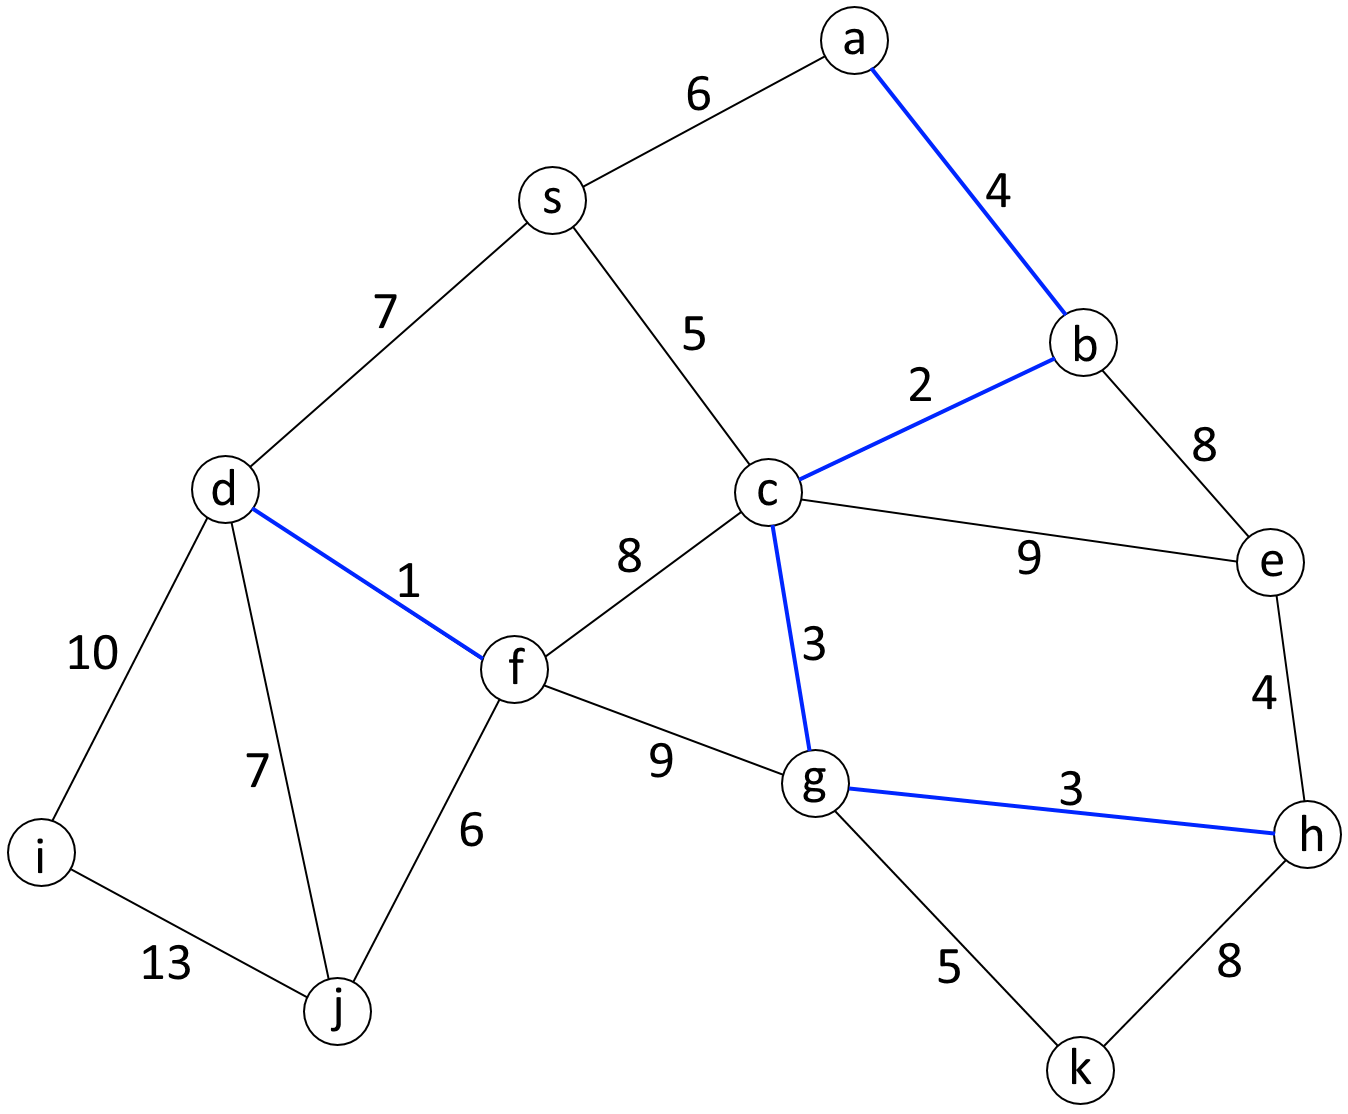
\includegraphics[width=.75\textwidth]{k5}
	
\end{frame}

\begin{frame}{Spannbäume – Beispiel Kruskal}
	
		\centering
		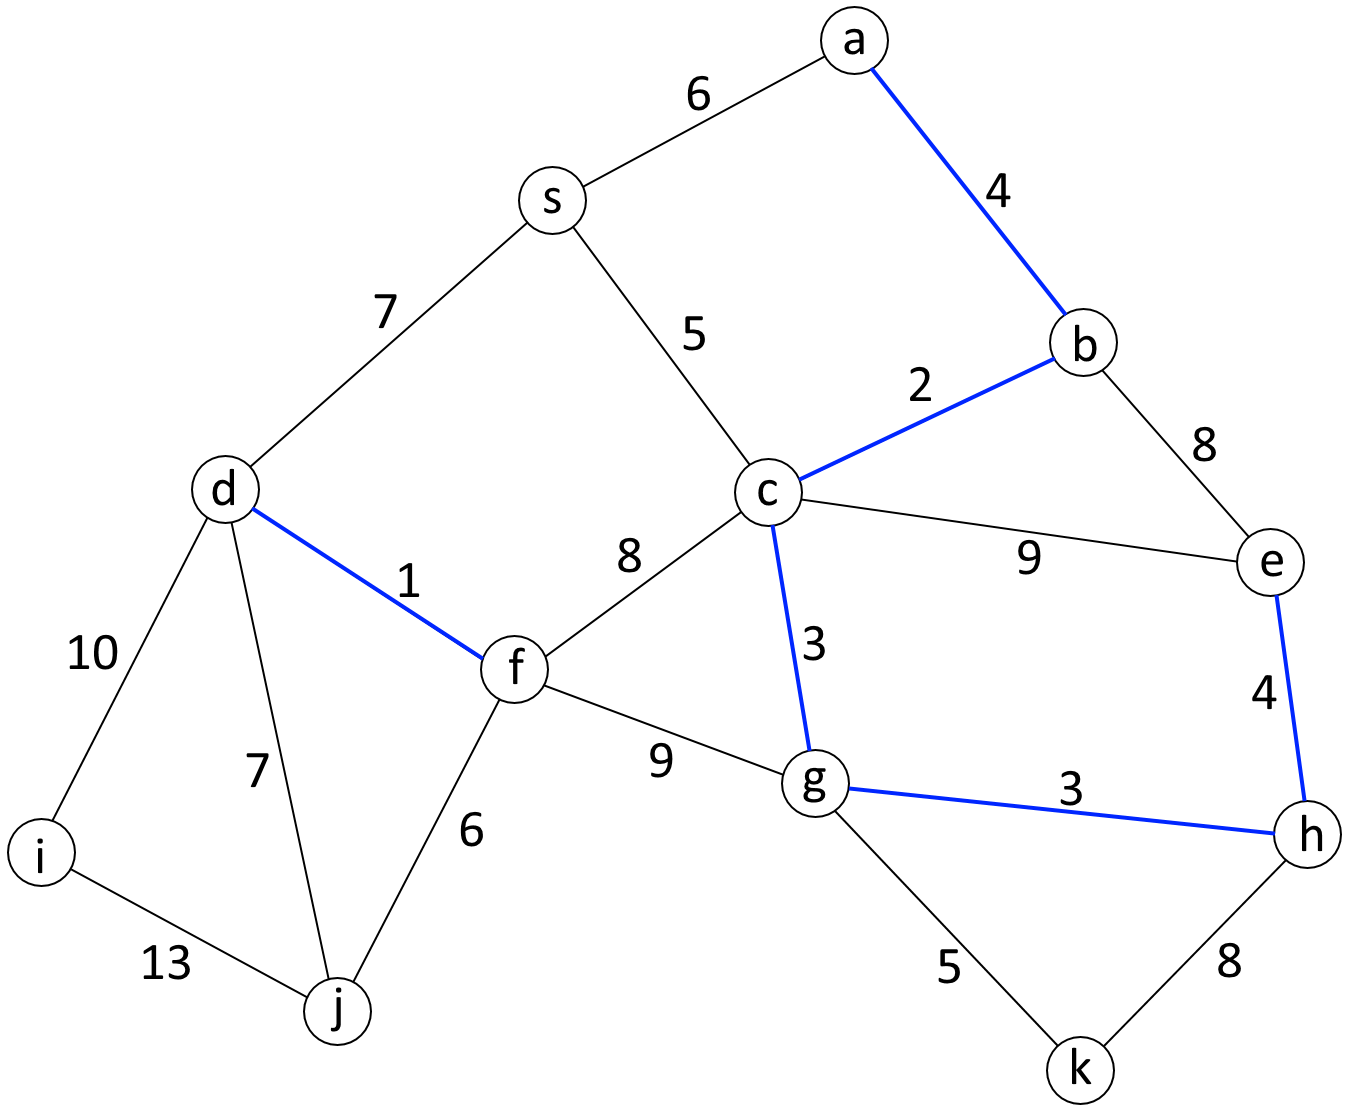
\includegraphics[width=.75\textwidth]{k6}
	
\end{frame}

\begin{frame}{Spannbäume – Beispiel Kruskal}
	
		\centering
		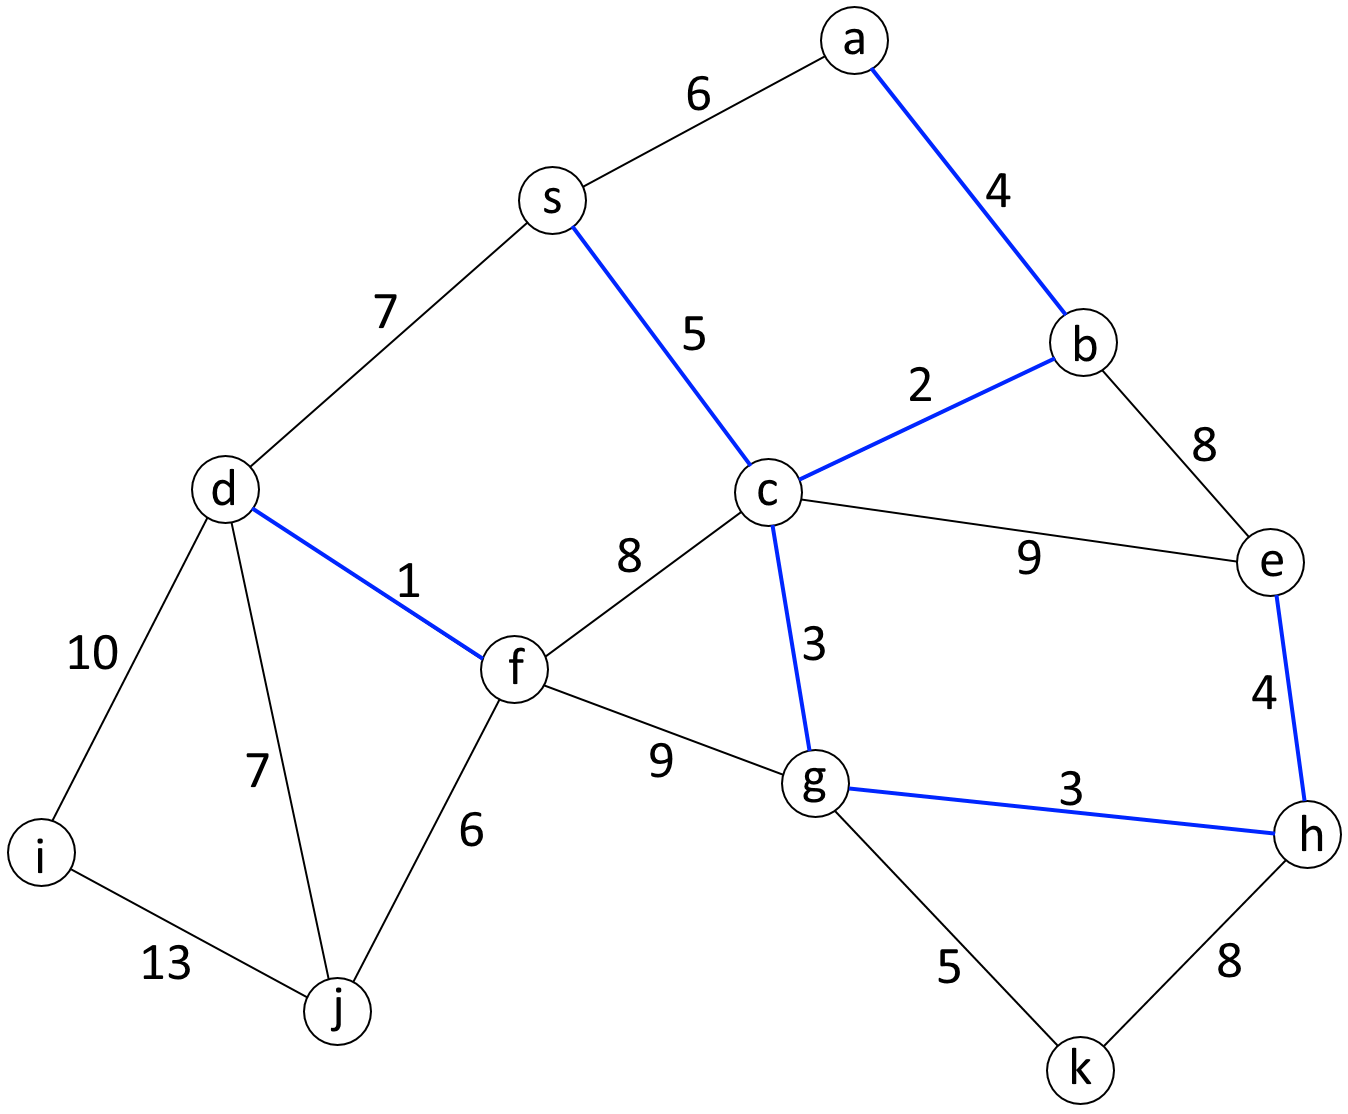
\includegraphics[width=.75\textwidth]{k7}
	
\end{frame}

\begin{frame}{Spannbäume – Beispiel Kruskal}
	
		\centering
		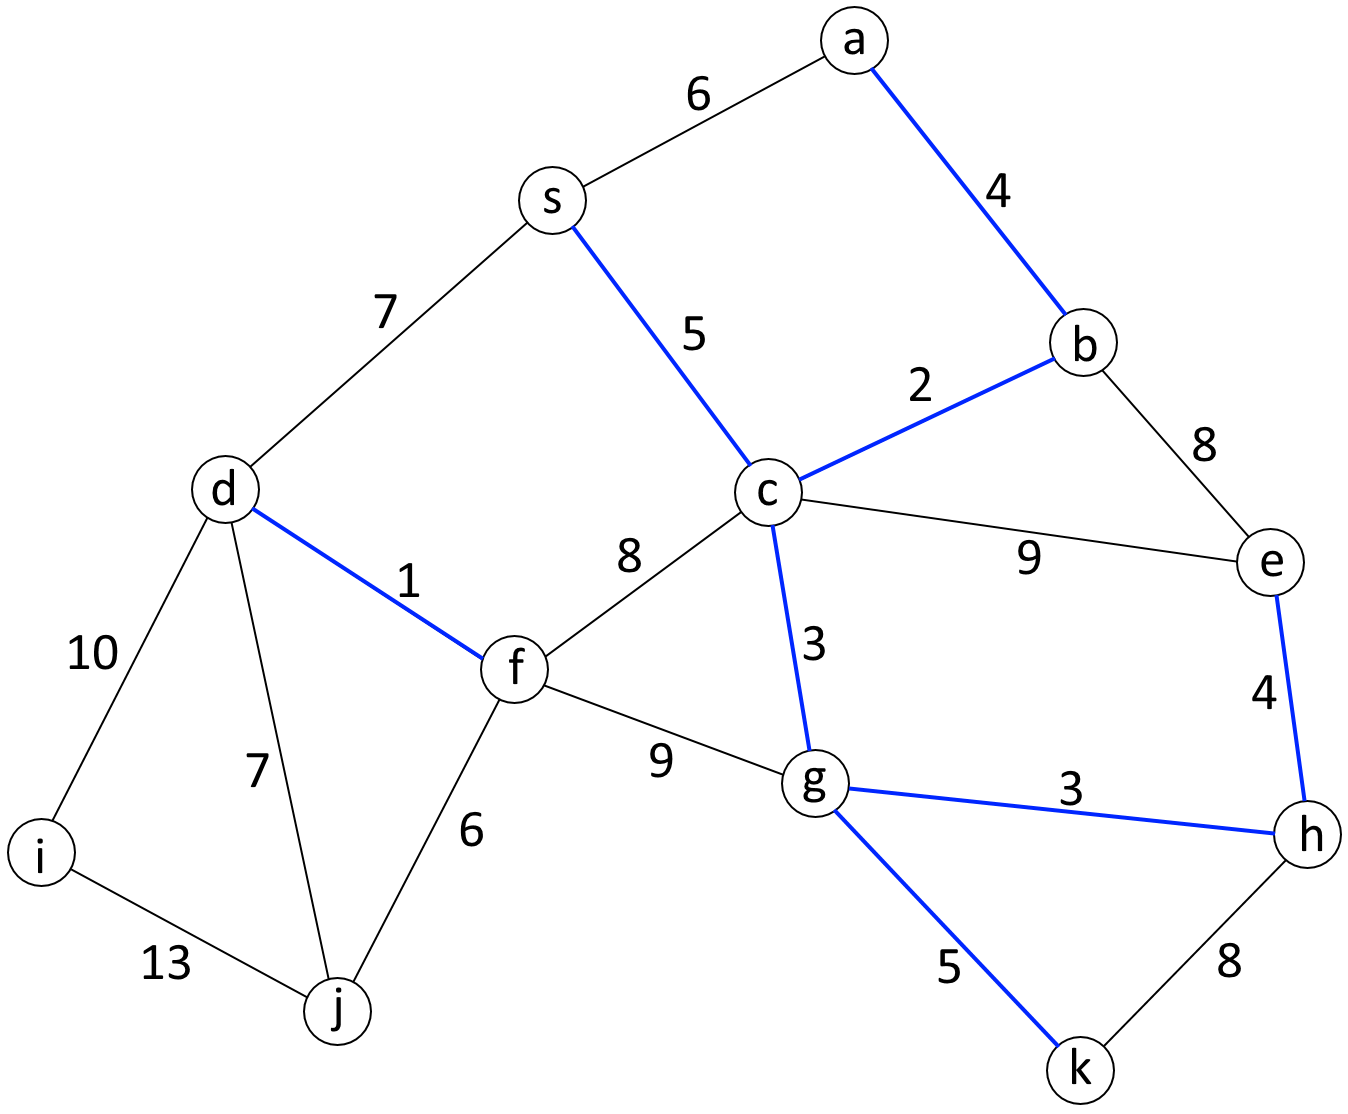
\includegraphics[width=.75\textwidth]{k8}
	
\end{frame}

\begin{frame}{Spannbäume – Beispiel Kruskal}
	
		\centering
		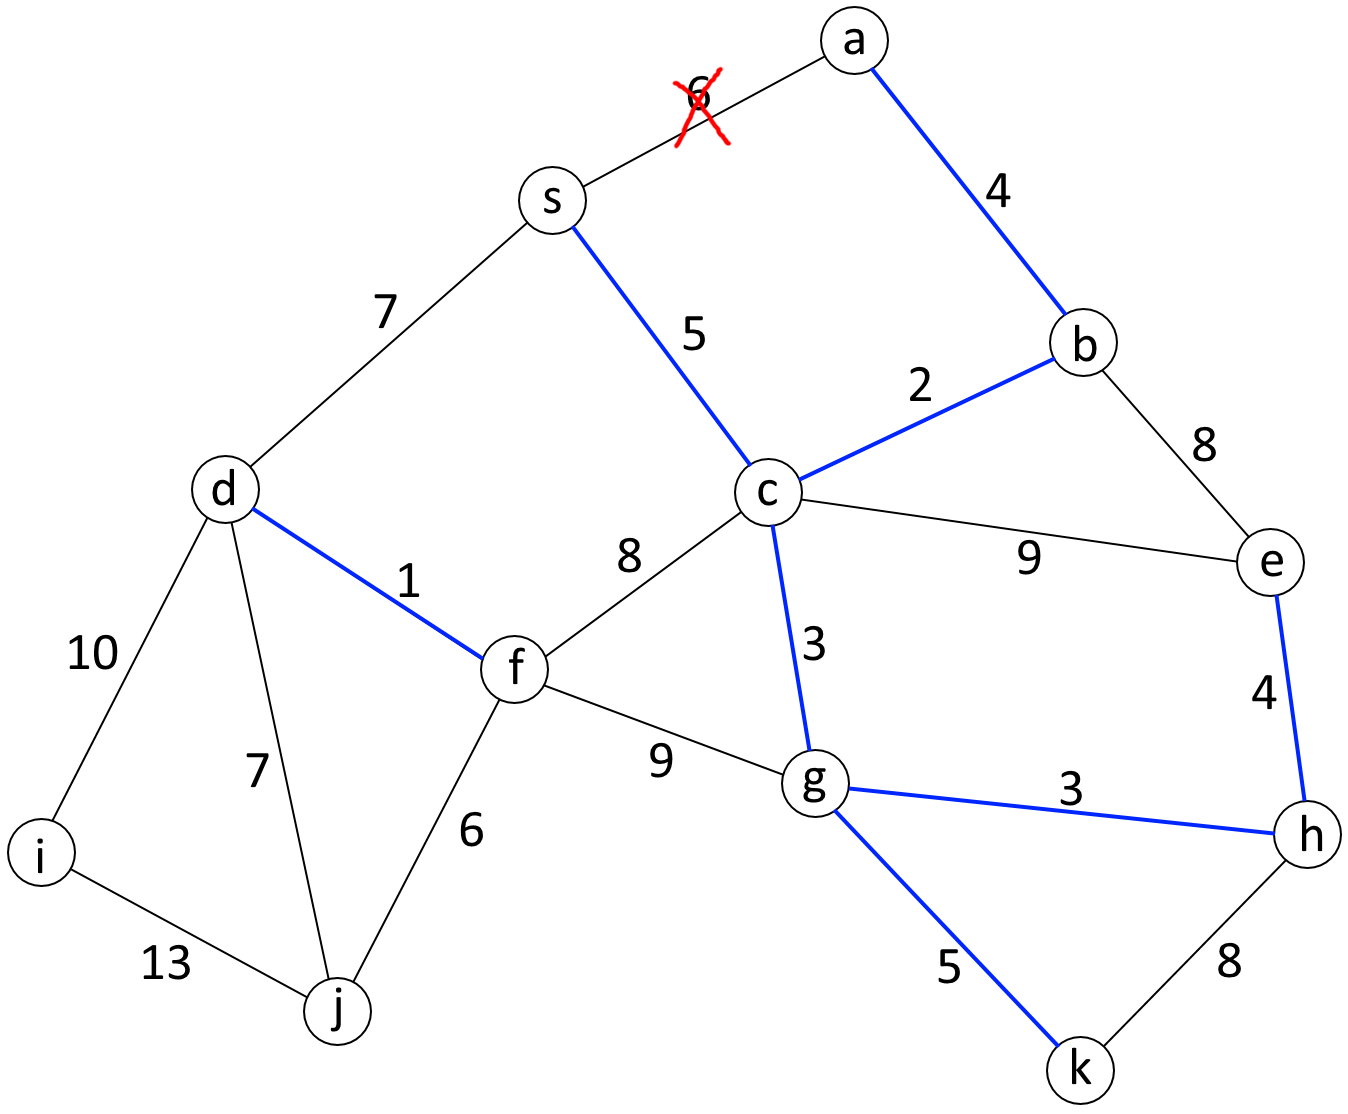
\includegraphics[width=.75\textwidth]{k9}
	
\end{frame}

\begin{frame}{Spannbäume – Beispiel Kruskal}
	
		\centering
		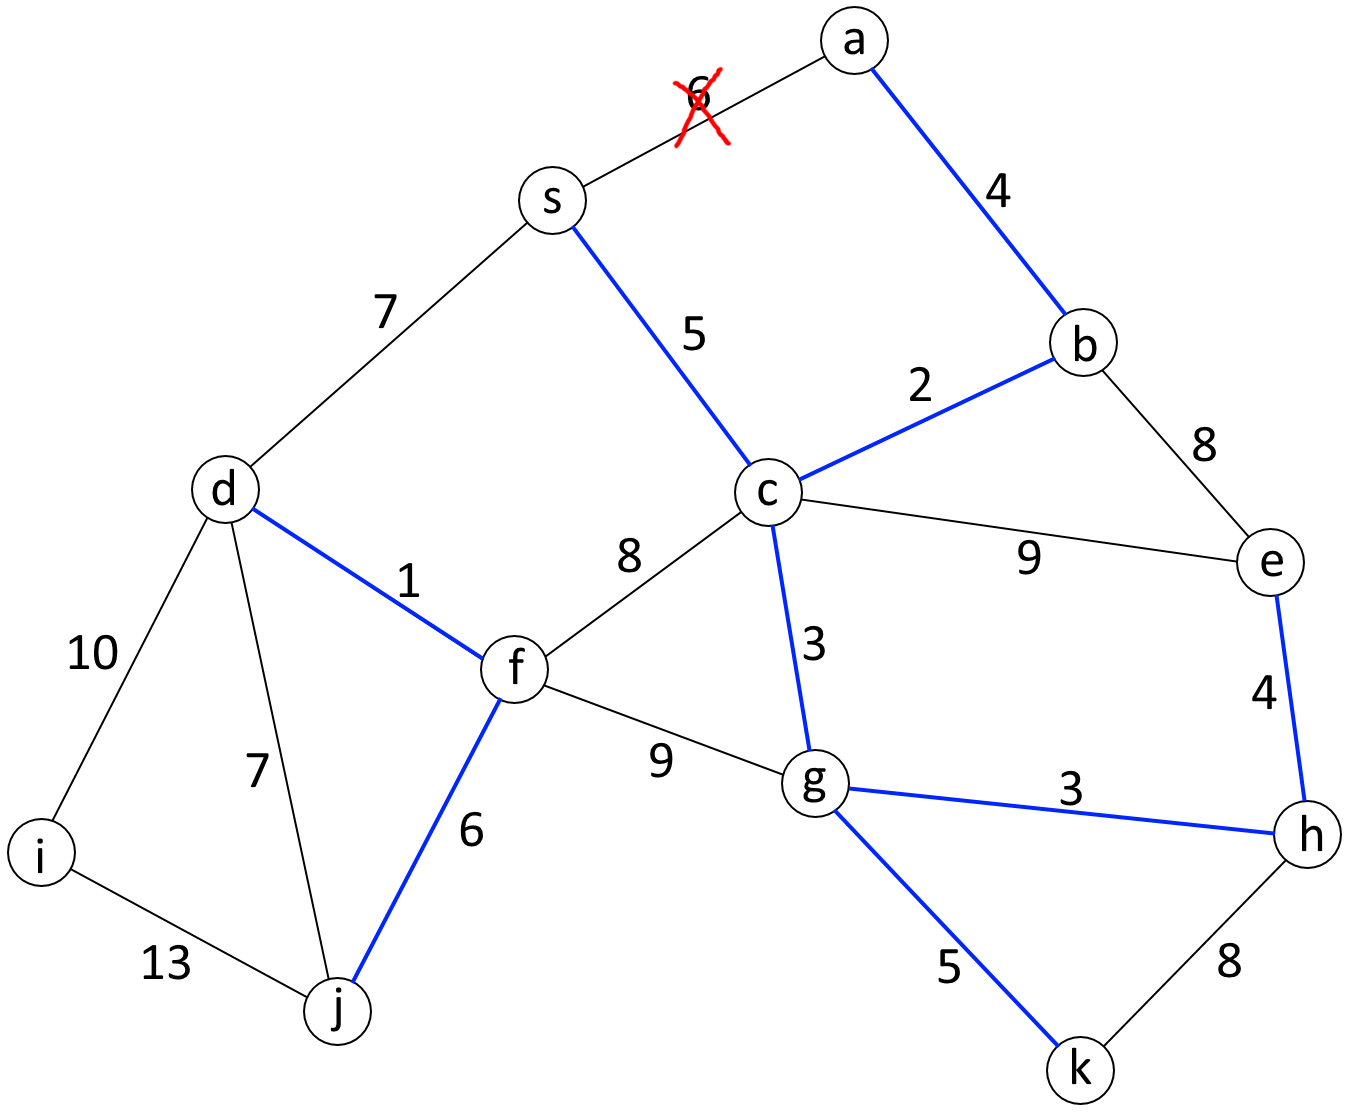
\includegraphics[width=.75\textwidth]{k10}
	
\end{frame}

\begin{frame}{Spannbäume – Beispiel Kruskal}
	
		\centering
		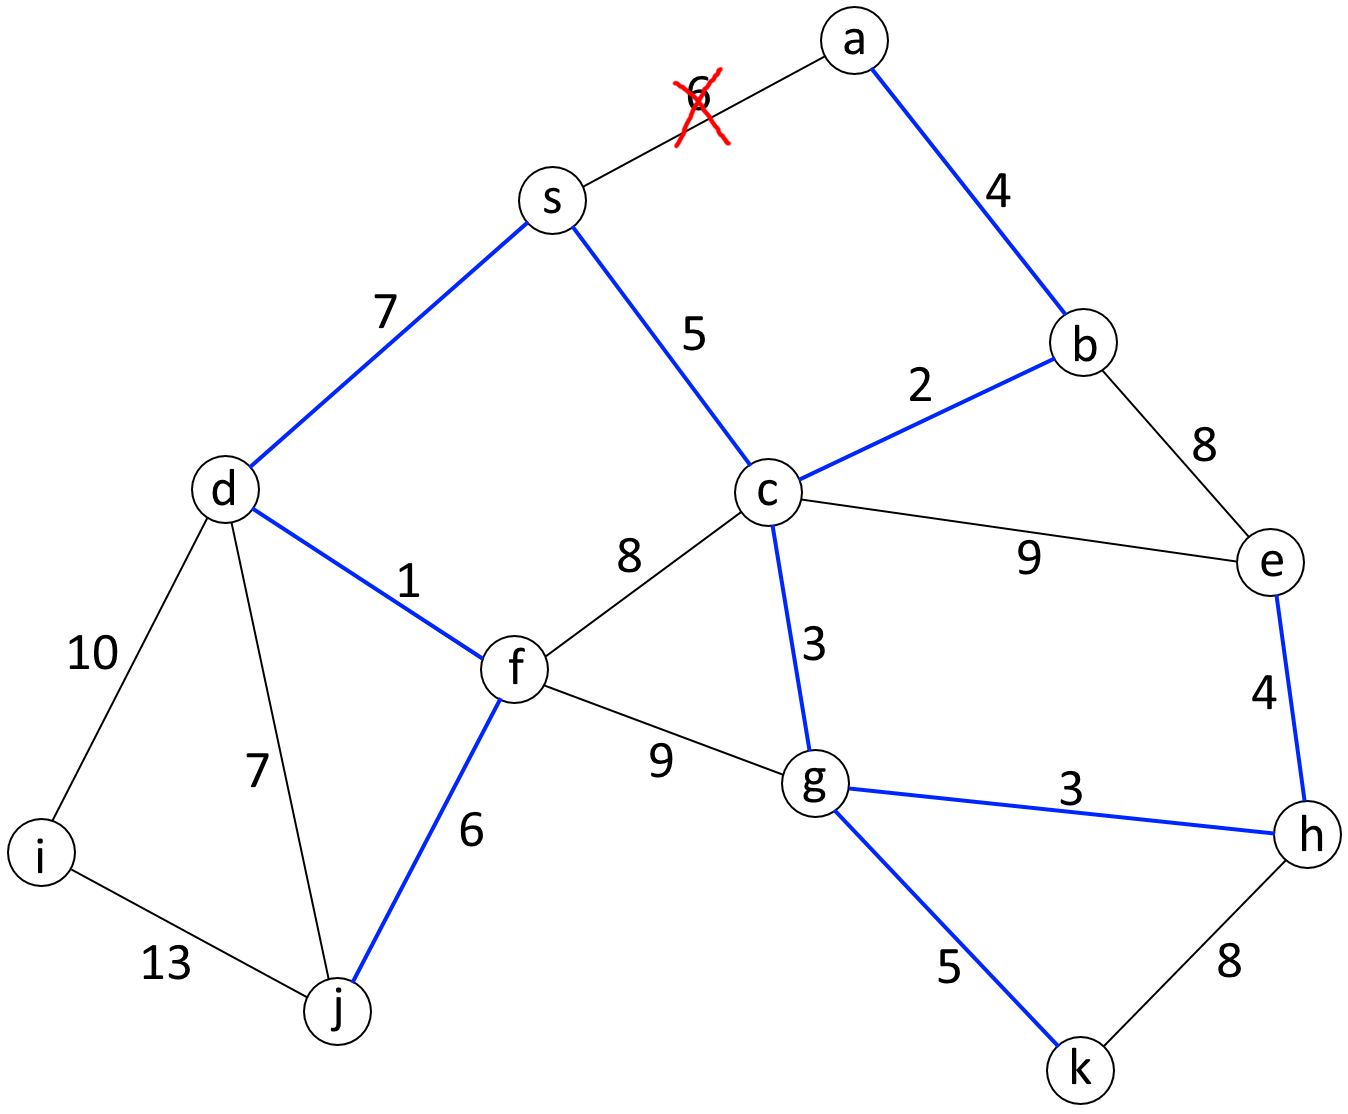
\includegraphics[width=.75\textwidth]{k11}
	
\end{frame}

\begin{frame}{Spannbäume – Beispiel Kruskal}
	
		\centering
		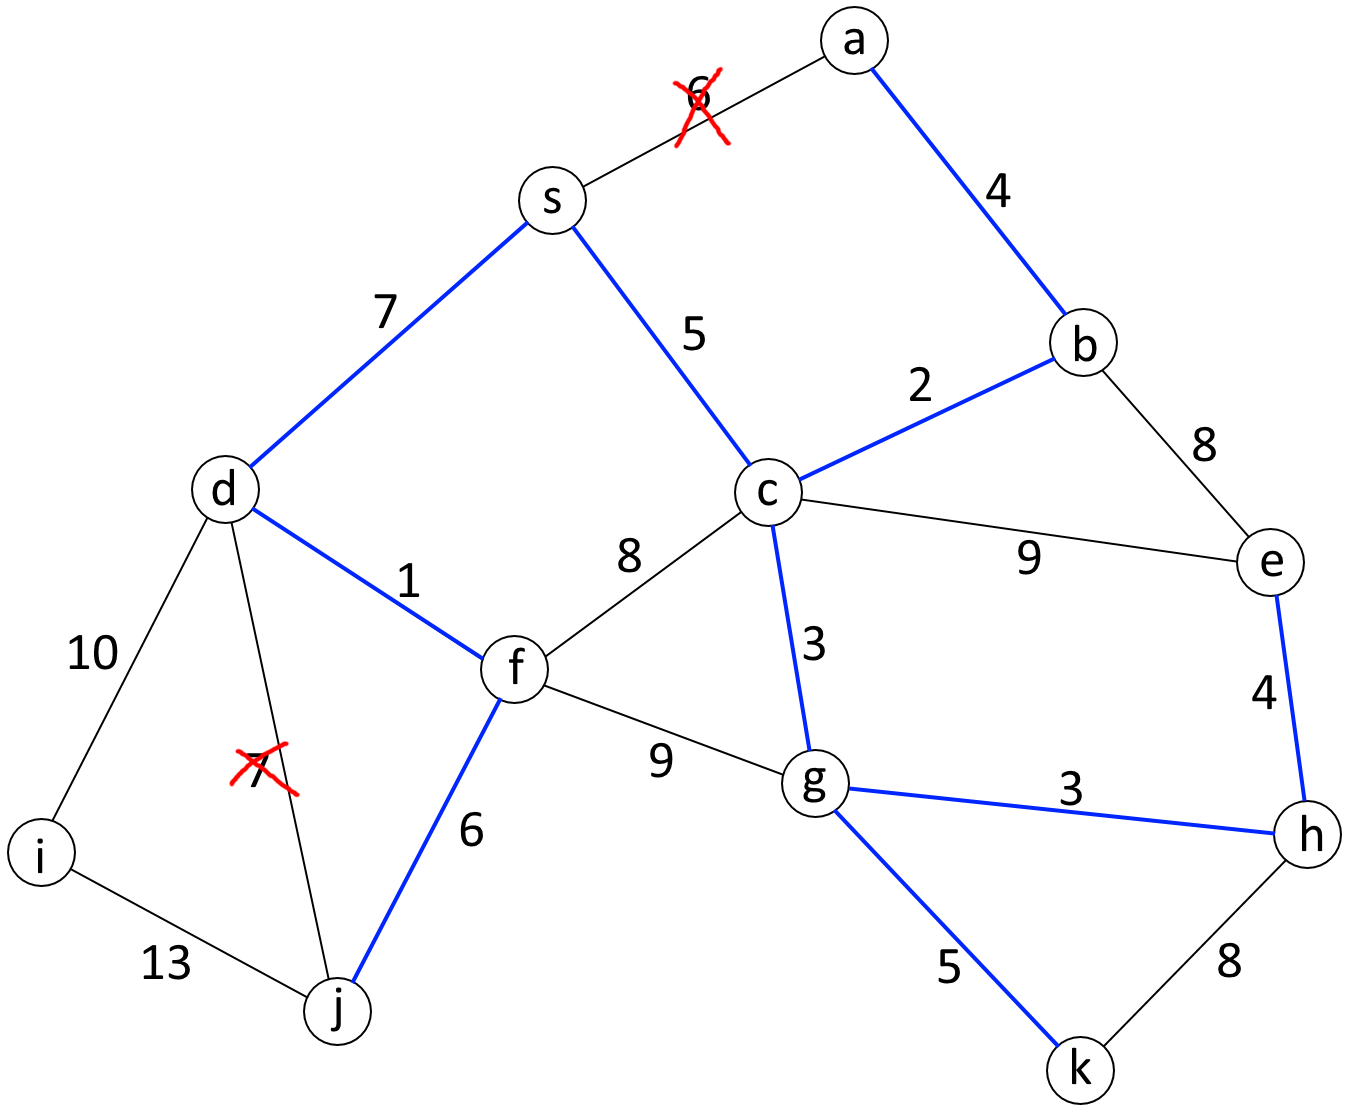
\includegraphics[width=.75\textwidth]{k12}
	
\end{frame}

\begin{frame}{Spannbäume – Beispiel Kruskal}
	
		\centering
		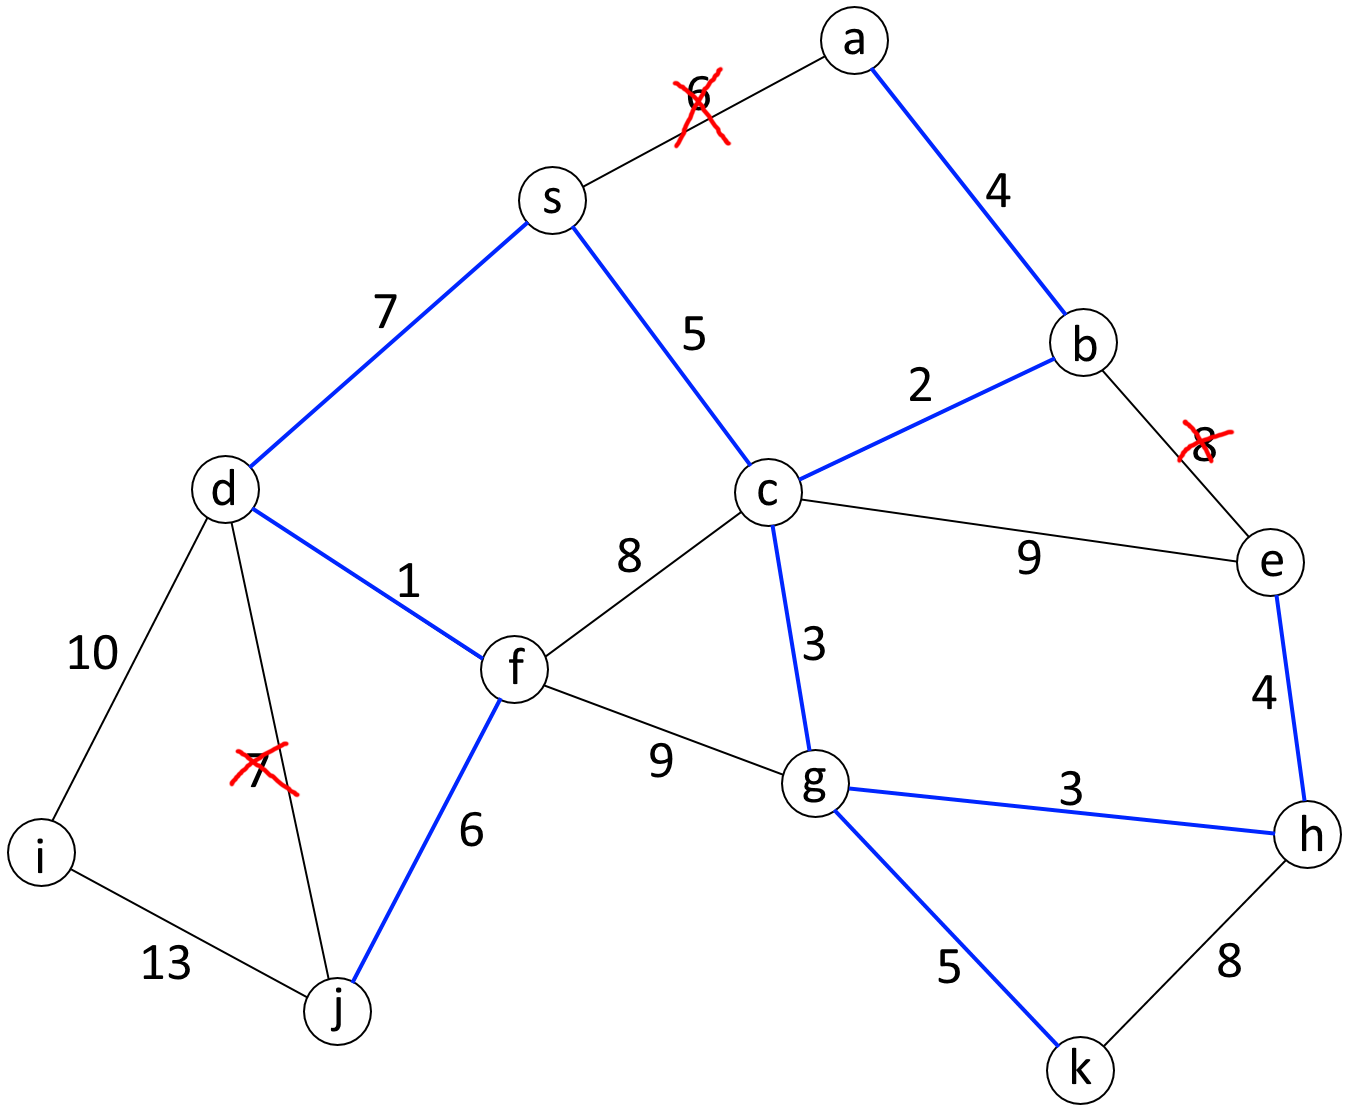
\includegraphics[width=.75\textwidth]{k13}
	
\end{frame}

\begin{frame}{Spannbäume – Beispiel Kruskal}
	
		\centering
		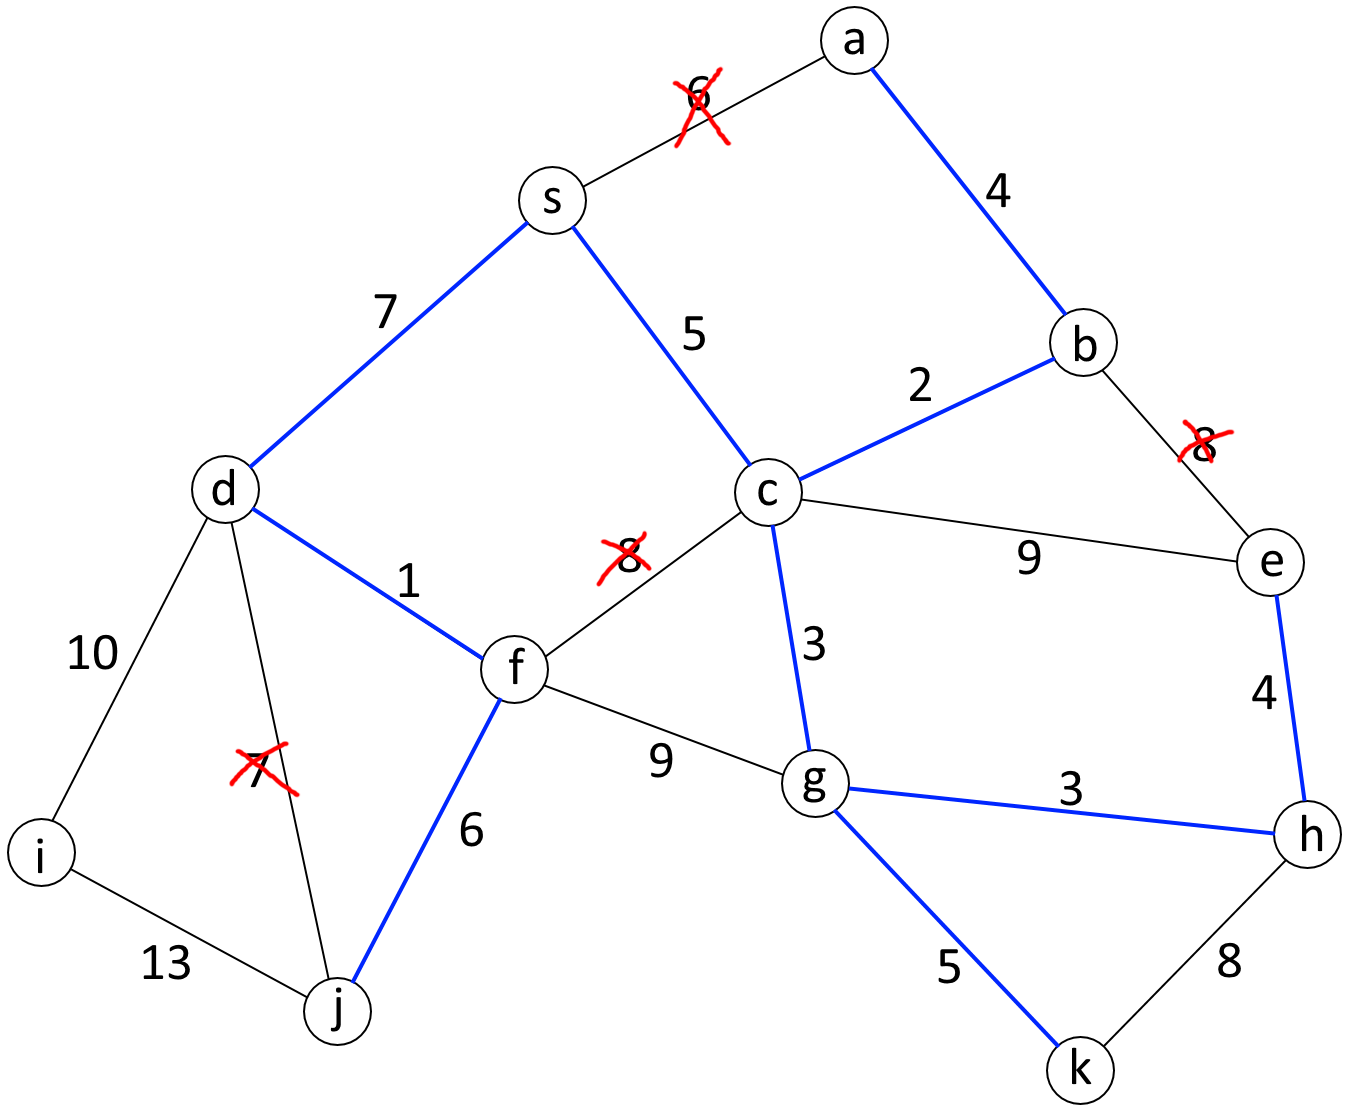
\includegraphics[width=.75\textwidth]{k14}
	
\end{frame}

\begin{frame}{Spannbäume – Beispiel Kruskal}
	
		\centering
		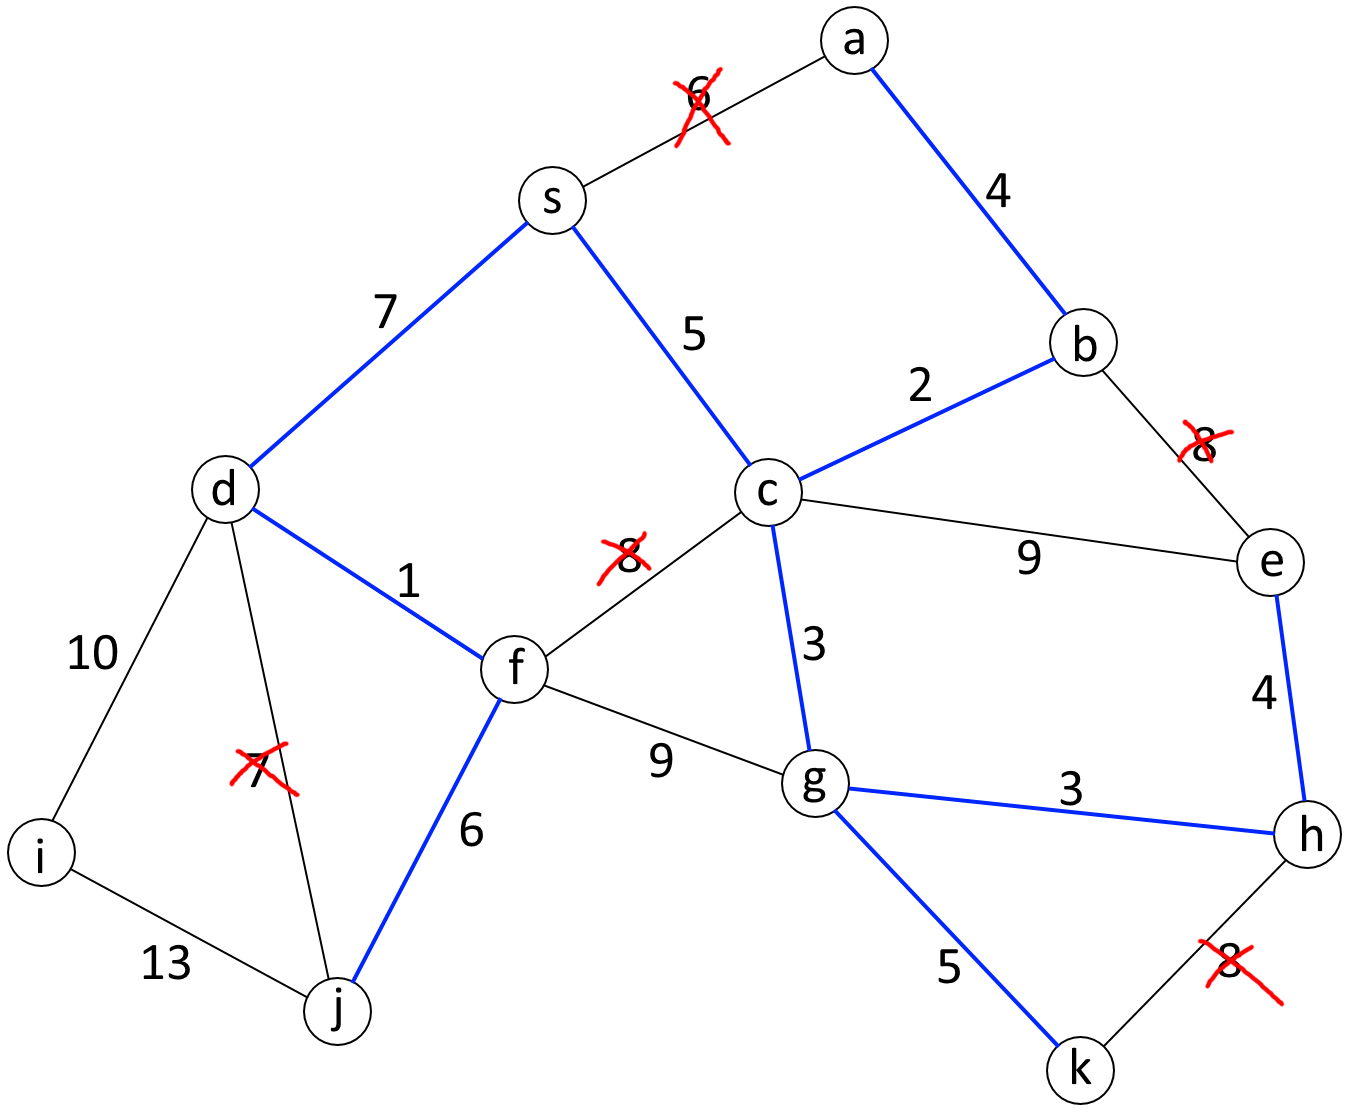
\includegraphics[width=.75\textwidth]{k15}
	
\end{frame}

\begin{frame}{Spannbäume – Beispiel Kruskal}
	
		\centering
		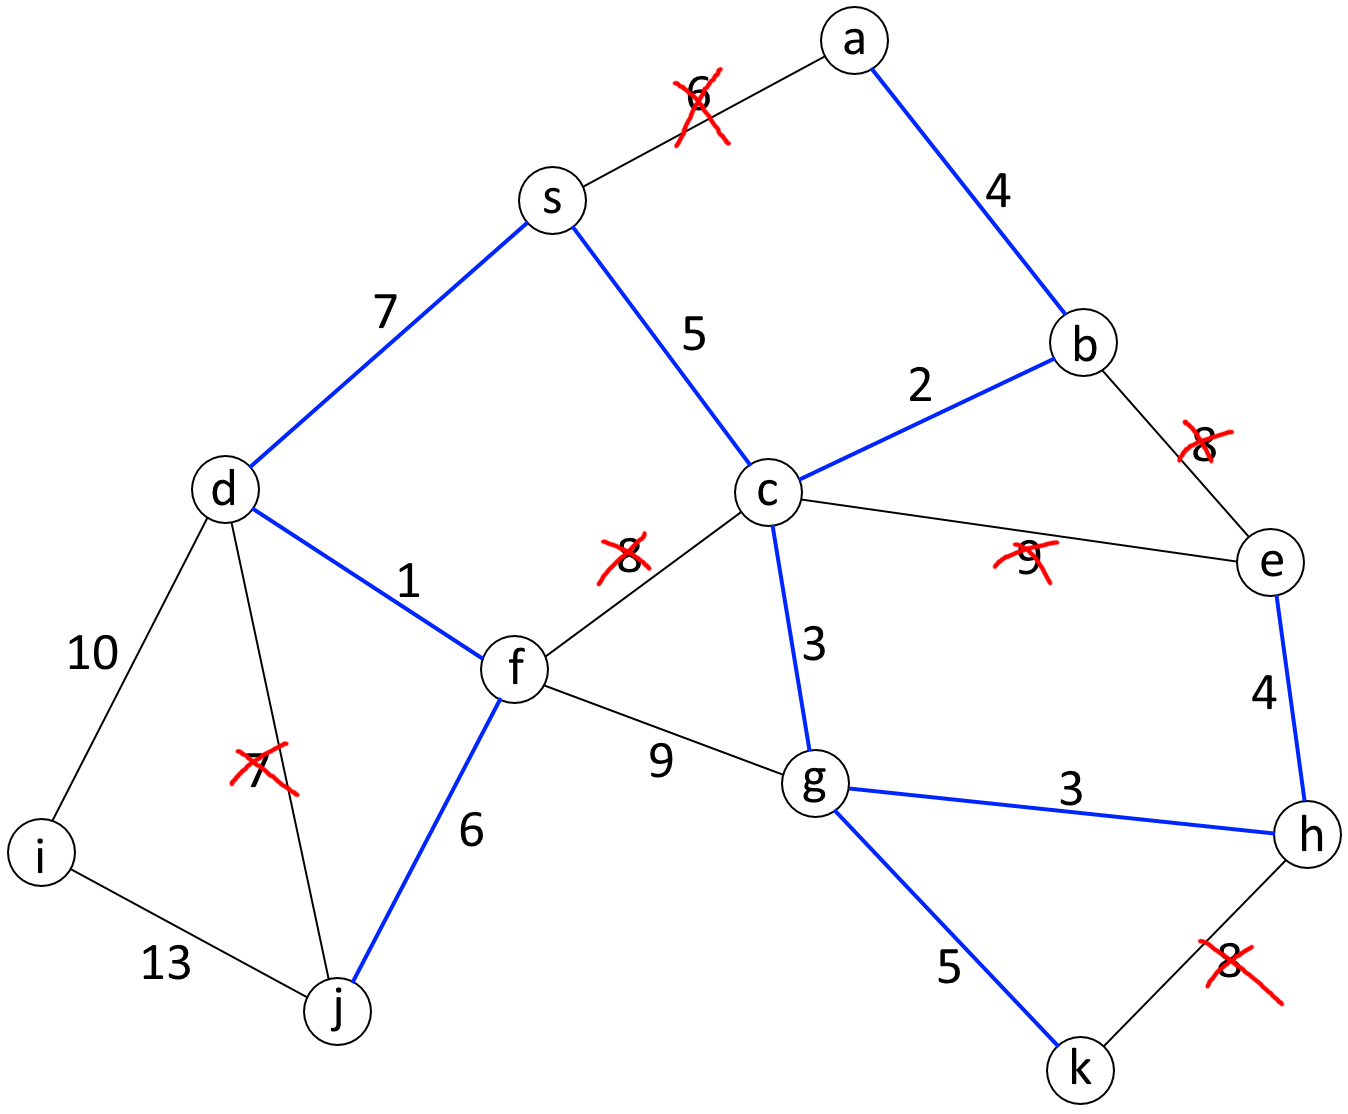
\includegraphics[width=.75\textwidth]{k16}
	
\end{frame}

\begin{frame}{Spannbäume – Beispiel Kruskal}
	
		\centering
		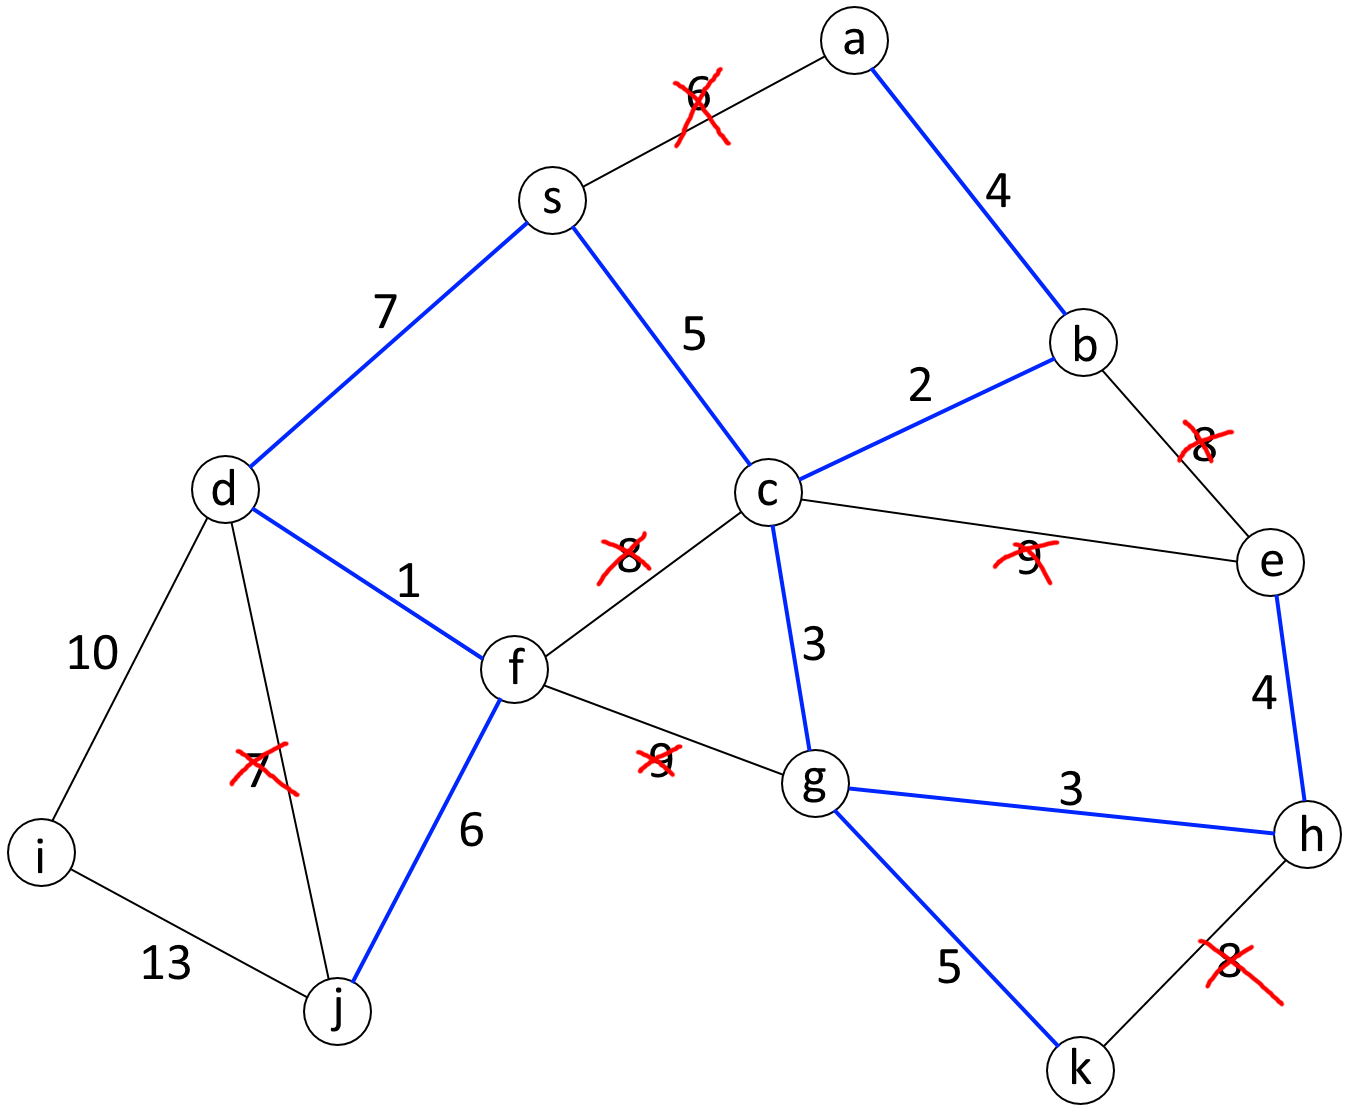
\includegraphics[width=.75\textwidth]{k17}
	
\end{frame}

\begin{frame}{Spannbäume – Beispiel Kruskal}
	
		\centering
		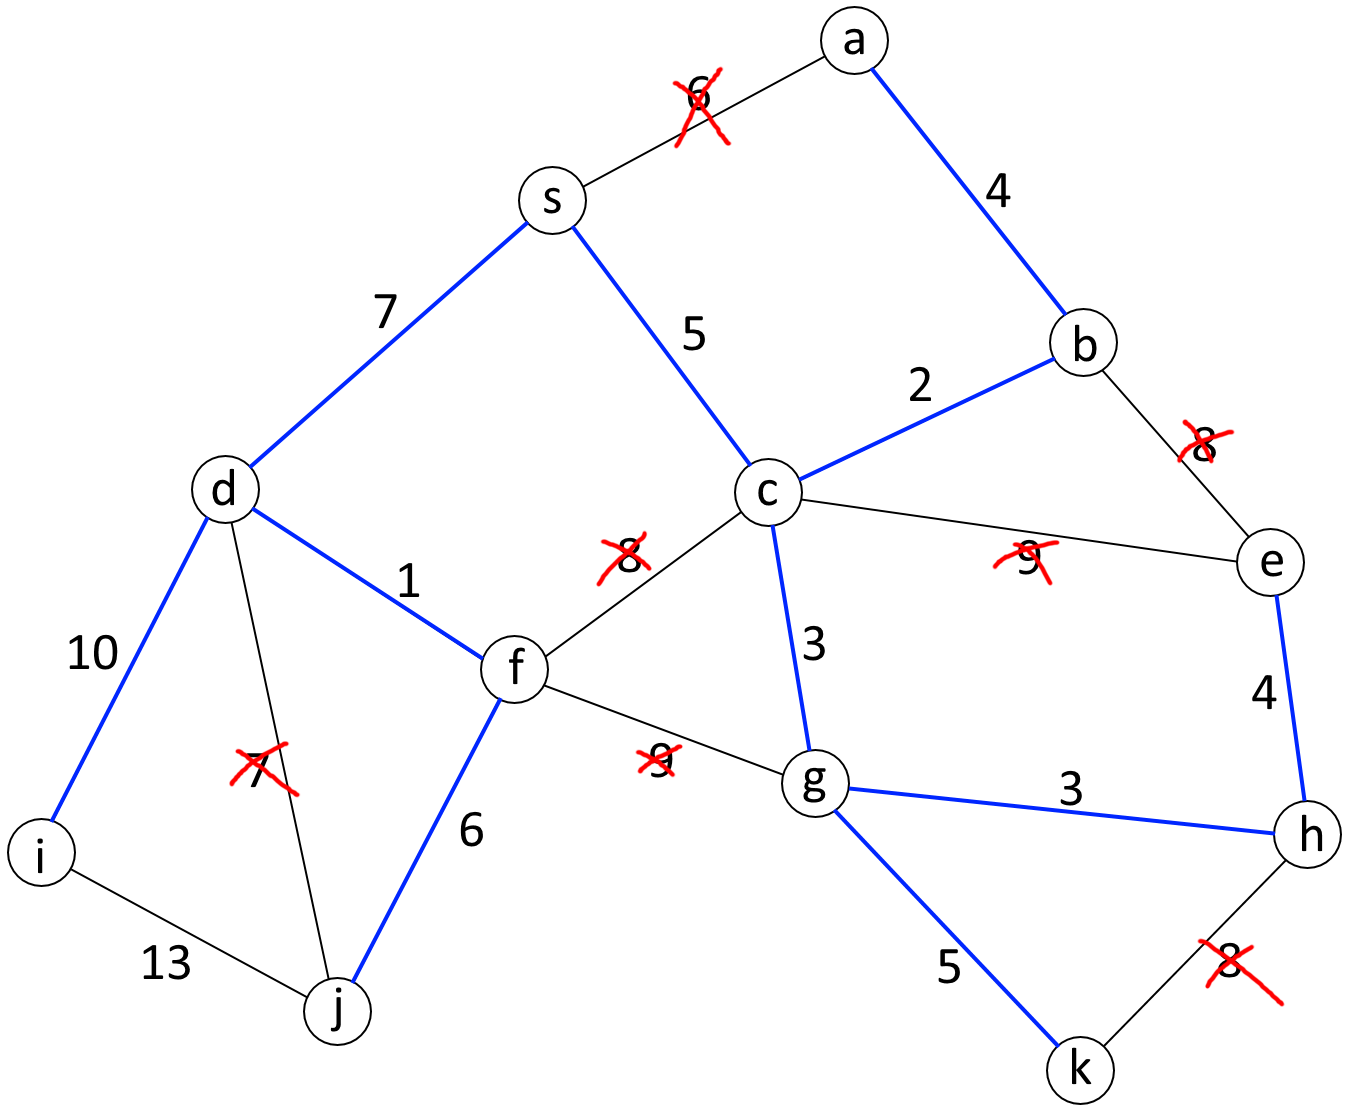
\includegraphics[width=.75\textwidth]{k18}
	
\end{frame}

\begin{frame}{{\hypertarget{label:afterEx2}{}Spannbäume – Beispiel Kruskal}}
		\centering
		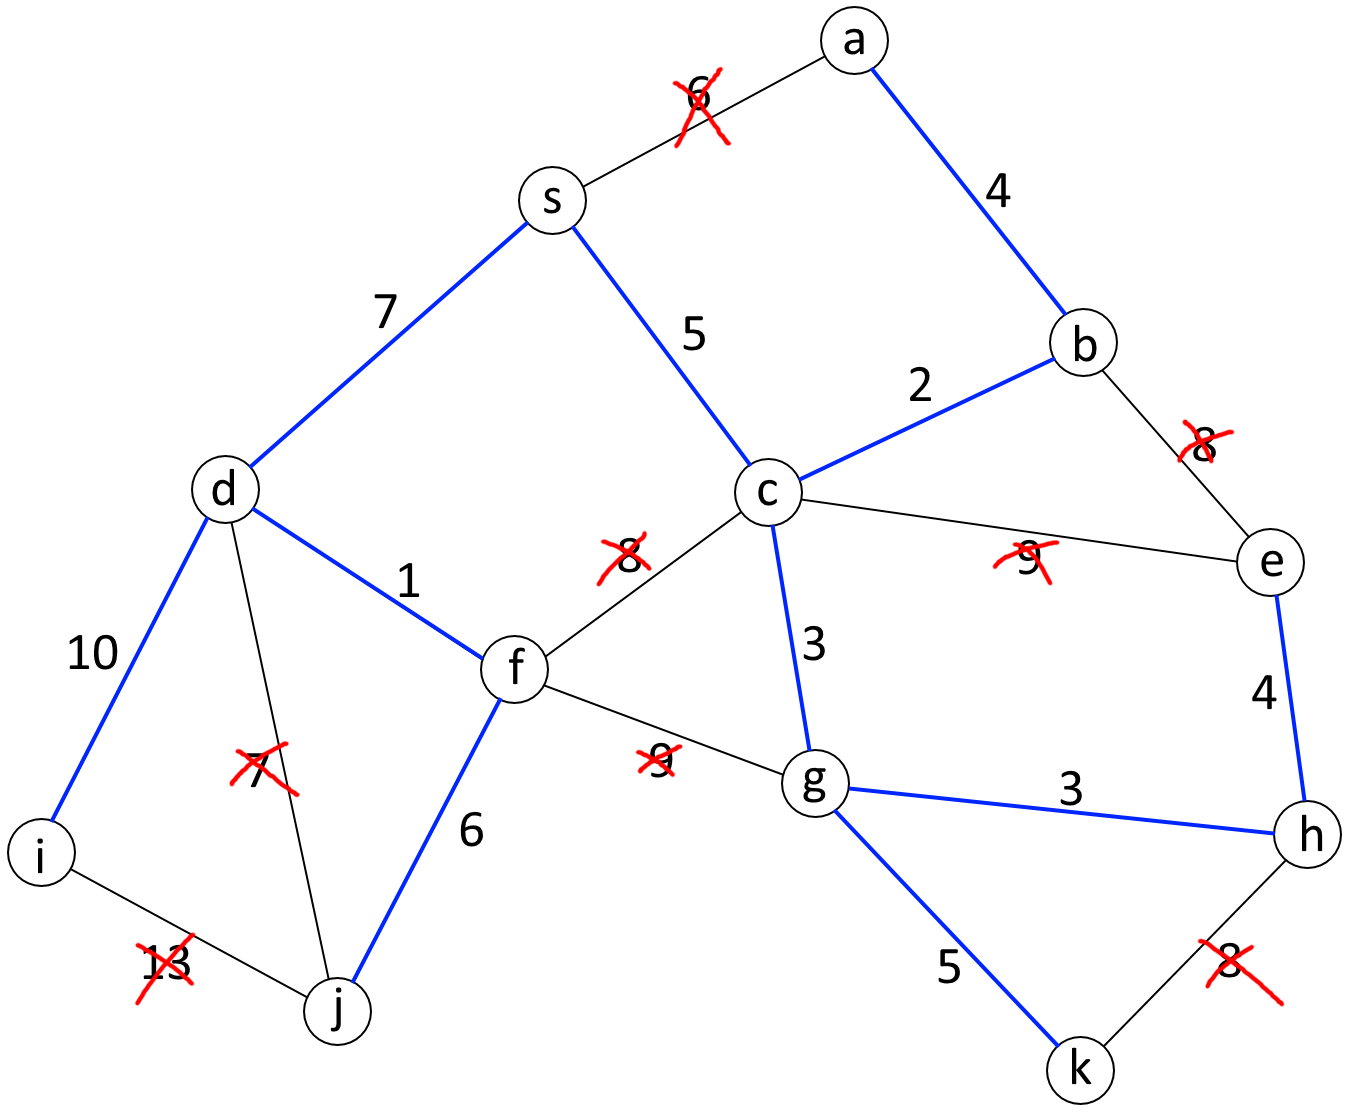
\includegraphics[width=.75\textwidth]{k19}
\end{frame}


\morescalingdelimiters
%TODO

\begin{frame}{Spannbäume – Kruskal}
	\textbf{Laufzeit von Kruskal} 
	\begin{itemize}
		\item[] $O(m \log m)$  \quad fürs Sortieren von $E$ 
		\pause
		\item[$+$] $O\left(m \cdot \alpha_T(m, n)\right) $ \quad für $m \times \text{find}() + n \times \text{union}()$ laut VL \\
		$\approx O(m \cdot 5) \quad ${\small (\textbf{Inv. Ackermannfunktion} $\alpha_T(\cdot,\cdot) \leq 5$ \ for all sane inputs)}
		\pause
		\item[$=$] $O(m \log m)$. \\
		Bei Kantengewichten in $\Z_+$ sogar schneller möglich. 
		%\item Satz aus Vorlesung: $m$-mal $find$ und $n$-mal $union$ läuft in $O(m \cdot \alpha_T(m, n))$, wobei $\alpha_T$ die \textbf{inverse Ackermannfunktion} ist \\
		%\pause
		%\impl Das \textbf{Sortieren} ist die \textbf{dominierende} Laufzeitkomponente
		%\pause
		%\item \textbf{Laufzeit} von Kruskal also $O(m \log m)$ (schneller bei \textbf{ganzzahligen} Kantengewichten) %Warum?
	\end{itemize}
\end{frame}

\begin{frame}[t]{Spannbäume}
	\FalseQuestionE{
			Die Union-Find-Datenstruktur bei Kruskals Algorithmus \\ repräsentiert den bisher gefundenen MST.
		}{
		Bloß interne Hierarchie für die Knoten. MST-Kanten tauchen da drin gar nicht auf.
	}
	\FalseQuestionE{
			Dijkstra ist zur Bestimmung eines MST bei gerichteten Graphen (mit nichtnegativen Kantengewichten) geeignet.
		}{
		Dijkstra bestimmt im Allgemeinen \textbf{keinen} \textbf{M}ST  {\small (und MST auf gerichteten Graphen nicht in dieser VL)}.
	}
	\TrueQuestionE{
			Sowohl der Algorithmus von Jarník-Prim als auch Kruskals Algorithmus funktionieren auch bei negativen Kantengewichten.
		}{\small (JP nach kleiner Anpassung)}
\end{frame}

\begin{frame}[t]{Spannbäume}
	\FalseQuestionE{
			Dijkstra funktioniert nicht, wenn negative Kantengewichte vorhanden sind.
		}{
		Dijkstra funktioniert nicht, wenn es negative \textbf{Zyklen} gibt \\ (\impl Endlosschleife). \\
		Ansonsten bestimmt Dijkstra auch \textbf{mit} negativen Kantengewichten \textbf{korrekte kürzeste Pfade}, aber in deutlich \textbf{schlechterer Laufzeit}. \\ (Achtung, \textbf{nicht} in VL gezeigt!)
	}
	\FalseQuestionE{
			Bellman-Ford bestimmt stets einen \textbf{beliebigen} Spannbaum.
		}{ 
		Nur wenn keine negativen Zyklen vorhanden sind!
	}
\end{frame}

\begin{frame}{Spannbäume}
	\underline{Aufgabe 2: Streaming MST} \\
	Gegeben sei ein ungerichteter zusammenhängender Graph $G = (V, E)$ mit $n$ Knoten, $m$ Kanten und positiven Kantengewichten. Die Knoten sind lokal gespeichert, die Kanten sind hingegen zunächst \textbf{unbekannt} und können nur \textbf{stückweise} (und in zufälliger Reihenfolge) aus dem Netz angefordert und im Speicher gehalten werden, da \textbf{nur} $O(n)$ \textbf{Platz} zur Verfügung steht. Gebt einen Algorithmus an, der unter diesen Einschränkungen einen MST von $G$ bestimmt.
\end{frame}

\begin{frame}{Spannbäume}
	\underline{Lösung zu Aufgabe 2} \\
	\begin{itemize}
		\item Verwende eine \textbf{Union-Find-Datenstruktur} (wie bei Kruskal). 
		\item Falls die neu angeforderte Kante \textbf{zwei Teilbäume verbindet}, füge sie hinzu. 
		\item Falls sie zwei Knoten \textbf{im selben} Teilbaum verbindet, füge sie provisorisch hinzu, schmeiße auf dem Pfad zwischen den Knoten die \textbf{schwerste Kante} raus. 
		\item \textbf{Laufzeit} in $O(m \cdot n)$, da bei der Bestimmung des Pfades maximal $n-1$ Kanten abgelaufen werden
	\end{itemize}
\end{frame}

\begin{frame}{Spannbäume}
	\underline{Aufgabe 3: Streaming MST mit Dünger} \\
	\hanging{ Wie bei Aufgabe 2: \newline
		Gegeben sei ein ungerichteter zusammenhängender Graph $G = (V, E)$ mit $n$ Knoten, $m$ Kanten und positiven Kantengewichten. Die Knoten sind lokal gespeichert, die Kanten sind hingegen zunächst \textbf{unbekannt} und können nur \textbf{stückweise} (und in zufälliger Reihenfolge) aus dem Netz angefordert und im Speicher gehalten werden, da \textbf{nur} $O(n)$ \textbf{Platz} zur Verfügung steht. Gebt einen Algorithmus an, der unter diesen Einschränkungen einen MST von $G$ bestimmt.
	} \\
	Er darf \textbf{nur $O(m \log n)$ Rechenzeit benötigen}.
\end{frame}

\begin{frame}{Spannbäume}
	\underline{Lösung zu Aufgabe 3} \\
	Wir besorgen uns Kanten-Pakete mit jeweils $n$ Kanten. \\
	Mit dem \textbf{ersten} Paket bestimmen wir (mit Kruskal) einen Minimum~Spanning~Forest (MSF) und entfernen alle anderen Kanten. \\
	\textbf{Restliche} Pakete behandeln wir so: \\
	\begin{itemize}
		\item Füge die $n$ neuen Kanten zum Graphen hinzu
		\item Bestimme auf diesem neuen Graphen mit (maximal) $2n-1$ Kanten einen MSF und entferne alle anderen Kanten
	\end{itemize}
	\impl \textbf{Laufzeit} in $O(m \log n)$, denn: \\
	Jeder dieser ca. $\frac{m}{n}$ Schritte benötigt Zeit in $O(n \log n)$.
\end{frame}

\begin{frame}{Spannbäume}
	\underline{Aufgabe 4: Ein Algorithmus mit Ecken und Kanten} \\
	Erneut betrachten wir einen ungerichteten zusammenhängenden Graphen $G = (V, E)$ mit $V = \{1...n\}$ und Kantengewichten in $\{1, 3\}$. $G$~sei in Form eines Adjazenzfeldes gegeben. Gebt einen Algorithmus an, der in $O(m)$ einen MST von $G$ berechnet (und begründet das Laufzeitverhalten).
\end{frame}

\begin{frame}{Spannbäume}
	\underline{Lösung zu Aufgabe 4} \\
	Getweaktes \textbf{Jarník-Prim}: \\
	\begin{itemize}
		\item Komplette PriorityQueue wäre \textbf{overkill} \impl \textbf{stattdessen} zwei einfache Queues $Q_1$ und $Q_3$ \quad (eine für jedes Kantengewicht)
		\item Merke zu jedem Knoten Pointer in die Queue (oder $\bot$)
		\implitem $insert$, $deleteMin$ und $decreaseKey$ in $O(1)$ durch einfaches Pointer-Umhängen
		\implitem \textbf{Laufzeit}: $O(n + m) = O(m)$ \\ (da für zusammenhängende Graphen $n \in O(m)$).
	\end{itemize}
	\forcenewline
	(Eine clevere Alternative wäre, die Kanten mit \textbf{Bucketsort} zu sortieren und dann \textbf{Kruskal} draufloszulassen \impl Laufzeit: $O\left(m \cdot \alpha_T(m, n)\right) \stackrel{\text{realistisch}}{\approx} O(5 \cdot m) = O(m)$. {\small Aber Achtung, $\alpha_T$ ist \textbf{nicht} konstant, deshalb „$\approx$“!})
\end{frame}



\iffalse

\begin{frame}{Graphen}
	\underline{Aufgabe 5: } \\
	Konstruiert einen gerichteten Graphen mit $n$ Knoten und negativen Kantengewichten (aber \textbf{ohne} negative Zyklen!) so, dass Dijkstra darauf eine Laufzeit in $\Theta(n^3\log n)$ erreicht.
\end{frame}

\fi

%\begin{frame}{Graphen}
%	\underline{Lösung zu Aufgabe 5} \\[0,125cm]
%	Grade keine Lust, ne Grafik zu erstellen. Ich kanns auswendig durch die Gegend schmieren. Außerdem sollst Du auch mal knobeln dürfen :D
%\end{frame}

\only<beamer:0>{\slideThanks}

\end{document}